\documentclass[12pt, twoside]{book}

\usepackage[paper=a4paper, top=1.5cm, bottom=2cm, left=2.5cm, right=2.5cm, headheight=15pt]{geometry}

\usepackage[utf8]{inputenc}
\usepackage[T1]{fontenc}		
\usepackage[english, francais]{babel}
\usepackage{csquotes}

\usepackage{siunitx}

\usepackage[dvipsnames]{xcolor}
\definecolor{darkgreen}{RGB}{0, 155, 85}


\usepackage{graphicx}
\usepackage{floatrow}
\usepackage{caption}
\usepackage{subfig}

\usepackage{standalone}

\usepackage{multirow}

\usepackage{array}
\newcolumntype{x}[1]{>{\centering\let\newline\\\arraybackslash\hspace{0pt}}m{#1}}
\usepackage{booktabs}

\usepackage{tikz}
\usetikzlibrary{calc, 3d, shadows, decorations, shapes.arrows, fadings}
\usepackage{pgfplots}
\usepackage{pgfplotstable}
\usepackage{forest}

\usepackage{amsmath}
\usepackage{amsthm}
\usepackage{amsfonts}
\usepackage{amssymb}
\usepackage{mathrsfs}
\usepackage{bm}
\usepackage{bbold}


\usepackage{palatino}

\setcounter{tocdepth}{2}
\usepackage{minitoc}
\setcounter{minitocdepth}{2}
\usepackage{tocbibind}

\usepackage[explicit]{titlesec}
\usepackage{bookmark}

\usepackage{chngcntr}
\counterwithout{footnote}{chapter}

\usepackage[
    backend=biber,
    style=authoryear,
    sorting=nty,
    maxbibnames=5,
    hyperref=true,
    backref=true,
    backrefstyle=all+,
    isbn=true,
    url=true,
    doi=true
]{biblatex}
\addbibresource{references.bib}

\usepackage[acronym, toc, automake=true]{glossaries}
\usepackage{imakeidx}
\makeindex[intoc]

\usepackage{hyperref}
\hypersetup{
    colorlinks=true,
    citecolor=black,
    filecolor=black,
    linkcolor=Blue,
    urlcolor=blue,
    pdftitle={Semantic aware quality evaluation of 3D polyhedral building models},
    pdfauthor={Oussama Ennafii},
    % pdfsubject={},
    pdfkeywords={3D urban modeling} {buildings} {quality assessment} {taxonomy} {classification} {error detection} {geometry} {aerial imagery} {Very High Spatial Resolution} {Digital Surface Model},
    pdfstartview={FitH},
    unicode=true
}

\usepackage[
    colorinlistoftodos,
    textsize=scriptsize
]{todonotes}
\newcommand{\addref}{\todo[color=red!40, inline]{Add reference.}}
\newcommand{\rewrite}[1]{\todo[color=green!40]{#1}}

\usepackage[useregional]{datetime2}


\usepackage{style/environments}
\usepackage{style/hacks}
\usepackage{style/glossaries}


\begin{document}
    \dominitoc
    \doparttoc
    \selectlanguage{english}
    \frontmatter
    \pagestyle{plain}
   
    \begin{titlepage}
    \newgeometry{
        inner=1cm,
        outer=1cm,
        bindingoffset=0.5cm,
        top=2cm,
        bottom=2cm,
    }
    \begin{center}
        \includestandalone[mode=buildnew, width=\textwidth]{figures/style/cover_logo}

        \vspace*{10mm}

        \begin{minipage}{.5\textwidth}
            \centering
            \textsc{LaSTIG -- STRUDEL,\\ Institut National de l'Information Géographique et Forestière (IGN)}
        \end{minipage}

        \vfill

        Dissertation submitted in partial fulfillment of the requirements for the degree of Doctor of Philosophy delivered by:

        \vspace*{5mm}

        \begin{Large}
            \textbf{Université Paris-Est -- MSTIC (ED532)}
        \end{Large}

        \vspace*{10mm}
        \begin{large}
            \textsc{Spetialty: Geographical Information Sciences and technologies}
        \end{large}
        \vspace*{10mm}

        \rule{\textwidth}{1.5pt}\\
        \begin{LARGE}
            \textsc{\textbf{Semantic aware quality evaluation of \acrshort*{acr::3d} polyhedral building models}}\\
        \end{LARGE}
        \vspace*{2.5mm}
        \begin{Large}
            \textsc{A scalable approach}
        \end{Large}
        \rule{\textwidth}{1.5pt}\\

        \vspace*{10mm}

        \begin{large}
            \textbf{Oussama \textsc{Ennafii}}
        \end{large}

        \vspace*{10mm}

        % defended \DTMdisplaydate{2019}{11}{29}{6} \\
        % at IGN, Saint-Mand\'e, France

        \vfill

        \begin{tabular}{l p{.7\textwidth} l}
            \multicolumn{2}{l}{\Large \textbf{Jury members}} & \\
            & & \\
             & \href{https://www.ipi.uni-hannover.de/fr.html?&L=1}{\color{black}\textbf{Franz \textsc{Rottensteiner}}} \dotfill & Reviewer \\
             & \href{https://perso.liris.cnrs.fr/gilles.gesquiere/wiki/doku.php?id=start}{\color{black}\textbf{Gilles \textsc{Gesquière}}} \dotfill & Reviewer \\
             & \href{http://imagine.enpc.fr/~marletr/}{\color{black}\textbf{Renaud \textsc{Marlet}}} \dotfill & Examiner \\
             & \href{https://research.utwente.nl/en/persons/george-vosselman}{\color{black}\textbf{George \textsc{Vosselman}}} \dotfill & Examiner \\
             & \href{http://recherche.ign.fr/labos/matis/~Le_Bris}{\color{black}\textbf{Arnaud \textsc{Le Bris}}} \dotfill & Supervisor \\
             & \href{http://recherche.ign.fr/labos/matis/~mallet}{\color{black}\textbf{Clément \textsc{Mallet}}} \dotfill & Advisor \\
             & \href{https://www-sop.inria.fr/members/Florent.Lafarge/}{\color{black}\textbf{Florent \textsc{Lafarge}}} \dotfill & Co-advisor \\
        \end{tabular}
    \end{center}
\end{titlepage}

    \null\vspace{\stretch {1}}
    \begin{flushright}
        tO WHOM it may concern ...
    \end{flushright}
\vspace{\stretch{2}}\null
    \leftchapter
    \chapter{\textsc{Abstract}}
        The automatic generation of 3D building models from geospatial data is now a standard procedure.
An abundant literature covers the last two decades and several softwares are now available.
However, urban areas are very complex environments.
Inevitably, practitioners still have to visually assess, at city-scale, the correctness of these models and detect frequent reconstruction errors.
Such a process relies on experts, and is highly time-consuming with approximately \SI[per-mode=repeated-symbol]{2}{\hour\per\km\squared\per\expert}.
This work proposes an approach for automatically evaluating the quality of 3D building models.
Potential errors are compiled in a novel hierarchical and modular taxonomy.
This allows, for the first time, to disentangle fidelity and modeling errors, whatever the level of details of the modeled buildings.
The quality of models is predicted using the geometric properties of buildings and, when available, Very High Resolution images and Digital Surface Models.
A baseline of handcrafted, yet generic, features is fed into a \acrlong*{acr::rf} or \acrlong*{acr::svm} classifiers.
Richer features, relying on graph kernels as well as Scattering Networks, were proposed to better take into consideration structure.
Both multi-class and multi-label cases are studied: due to the interdependence between classes of errors, it is possible to retrieve all errors at the same time while simply predicting correct and erroneous buildings.
The proposed framework was tested on three distinct urban areas in France with more than 3,000 buildings.
80\%-99\% F-score values are attained for the most frequent errors.
For scalability purposes, the impact of the urban area composition on the error prediction was also studied, in terms of transferability, generalization, and representativeness of the classifiers.
It shows the necessity of multi-modal remote sensing data and mixing training samples from various cities to ensure a stability of the detection ratios, even with very limited training set sizes.

    \selectlanguage{french}
    \chapter{\textsc{Résumé}}
        La génération automatique de modèles de construction 3D à partir de données géospatiales est maintenant une procédure standard.
Une littérature abondante couvre les deux dernières décennies et plusieurs solutions logicielles sont maintenant disponibles.
Cependant, les zones urbaines sont des environnements très complexes.
Inévitablement, les producteurs de données doivent encore évaluer visuellement, à l'échelle de villes, l'exactitude de ces modèles et détecter les erreurs fréquentes de reconstruction.
Un tel processus fait appel à des experts et prend beaucoup de temps, soit environ \SI[per-mode=repeated-symbol]{2}{\hour\per\km\squared\per\expert}.
Cette thèse propose une approche d'évaluation automatique de la qualité des modèles de bâtiments 3D.
Les erreurs potentielles sont compilées dans une nouvelle taxonomie hiérarchique et modulaire.
Cela permet, pour la première fois, de séparer erreurs de fidélité et de modélisation, quelque soit le niveau de détail des bâtiments modélisés.
La qualité des modèles est estimée à l'aide des propriétés géométriques des bâtiments et, lorsqu'elles sont disponibles, d'images géospatiales à très haute résolution et des modèles numériques de surface.
Une base de référence de caractéristiques \textit{ad hoc} génériques est utilisée en entrée d'un classificateur par Random Forest ou par Séparateurs à Vaste Marge.
Des attributs plus riches, s'appuyant sur des noyaux de graphes ainsi que sur des réseaux de type Scattering ont été proposées pour mieux prendre en compte la structure dans la donnée 3D.
Les cas multi-classes et multi-étiquettes sont étudiés séparément: de par l'interdépendance entre les classes d'erreurs, il est possible de détecter toutes les erreurs en même temps tout en prédisant au niveau sémantique le plus simple des bâtiments corrects et erronés.
Le cadre proposé dans cette thèse a été testé sur trois zones urbaines distinctes en France avec plus de 3 000 bâtiments étiquetés manuellement.
Des valeurs de F-score élevées sont atteintes pour les erreurs les plus fréquentes (80\%-99\%).
Pour une problématique de passage à l’échelle, l'impact de la composition de la zone urbaine sur la prédiction des erreurs a également été étudié, en termes de (i) transférabilité, de (ii) généralisation et de (iii) représentativité des classificateurs.
Cette étude montre la nécessité de disposer de données de télédétection multimodale et de mélanger des échantillons d'entraînement provenant de différentes villes pour assurer une stabilité des taux de détection, même avec des tailles d'ensembles d'entraînement très limitées.

    \chapter{\textsc{Résumé étendu}}
        \begin{french}
    Un chapitre long.
\end{french}
    \selectlanguage{english}
    \chapter{\textsc{Acknowlegements}}
        These are the acknowledgements.


    \printglossary[type=\acronymtype]
    \printglossary

    \mtcaddchapter
    \tableofcontents
    \mtcaddchapter
    \listoffigures
    \mtcaddchapter
    \listoftables
    \mtcaddchapter

    \mainmatter
    \rightchapter

    \chapter{\textsc{Introduction}}
        \label{chap::introduction}
        \minitoc

\vfill

The goal of this introduction is to acquaint the reader with concepts that are manipulated in this study.
In Section~\ref{sec::introduction::urban_3d_reconstruction}, we illustrate what is meant by urban \index{urban!\gls{acr::3d}!model}\gls{acr::3d} models, and specifically, \index{building!model} building \gls{acr::3d} models.
The role of this chapter is also to motivate the need for a semantic \index{building!model!evaluation}evaluation of such models.
Indeed, in Section~\ref{sec::introduction::building_model_evaluation}, we address different aspects of building \index{urban!\gls{acr::3d}!model}\gls{acr::3d} model inspection and the issues it raises.
We conclude by stating our contributions (cf. Section~\ref{sec::introduction::contributions}) and announcing the structure of the thesis (cf. Section~\ref{sec::introduction::structure_of_thesis}).

\clearpage

\section{Urban \texorpdfstring{\acrshort*{acr::3d}}{3D} reconstruction}
    \label{sec::introduction::urban_3d_reconstruction}
    Object \index{\gls{acr::3d}!reconstruction}\gls{acr::3d} reconstruction is a wide research field that interests \index{photogrammetry}photogrammetry, \index{computer vision}computer vision and \index{computer graphics}computer graphics communities.
    Starting from some input sensor data\footnote{which usually are unstructured.} (\gls{acr::lidar} point clouds or multiview stereo images), the goal is to model the \gls{acr::3d} surface that bounds an object of interest.
    In \index{\acrshort{acr::gis}}\acrfull{acr::gis}, \gls{acr::3d} data is instrumental to model the Earth surface at different spatial scales.
    In particular, this field takes a special interest in \index{urban!area}urban areas.
    Objects present in such scenes usually obey some specific rules which constrain their shape.
    In this section, we discuss applications of \index{urban!\gls{acr::3d}!model}urban \gls{acr::3d} models (cf. Section~\ref{subsec::introduction::urban_3d_reconstruction::applications}).
    We afterwards tackle the subject of \index{building!\gls{acr::3d}!model} \gls{acr::3d} building modeling and the issues it raises (cf. Section~\ref{subsec::introduction::urban_3d_reconstruction::building_3d_modeling}).
    This section ends in Section~\ref{subsec::introduction::urban_3d_reconstruction::challenges} with a list of some of the important technical challenges that are still to be overcome in this domain.

    \subsection{Applications of urban \texorpdfstring{\gls*{acr::3d}}{3D} models}
        \label{subsec::introduction::urban_3d_reconstruction::applications}
        In the following, we present a brief survey of \index{urban!model!application} urban \gls{acr::3d} models applications.
        A more comprehensive study was presented in~\parencite{biljecki2015applications}.
        The goal is to persuade the reader of the relevance of urban \index{urban!\gls{acr::3d}!model}\gls{acr::3d} modeling and how much affected everybody can be.
        Indeed, urban \gls{acr::3d} models answer to various needs: administrative, environmental, scientific and societal.

        \subsubsection{Administration related challenges}
            Administrative bodies need to document land usage in an effort to efficiently manage territories.
            Cadastre is a tool that helps track ownership and usage of a each land parcel.
            Cadastral records are produced and maintained to define fiscal policies.
            Cadastral data, since conception, came in the form of \index{\gls{acr::2d}!maps}\gls{acr::2d} maps~\parencite{billen20033d}.
            Although many urban planning norms were always formulated taking into account height or depth information \parencite{brasebin20183d}, the need for a \index{\gls{acr::3d}!cadastre}\gls{acr::3d} cadastral management was made relevant with the advent of complex architectural features~\parencite{biljecki2015applications}.
            To illustrate this case, we show, in Figure~\ref{fig::3d_cadastre_need_example}, how \gls{acr::2d} cadastral maps are insufficient when it comes to modeling overhangs.\\
            \begin{figure}[!htpb]
                \centering
                \includegraphics[width=.9\textwidth]{images/introduction/3d_model_applications/3d_cadastre}
                \caption[
                    Example of a problematic situation where \acrshort*{acr::3d} cadastre would be of help and \acrshort*{acr::2d} maps fail.
                ]{
                    \label{fig::3d_cadastre_need_example}
                    Example of a problematic situation where \acrshort*{acr::3d} cadastre would be of help and \acrshort*{acr::2d} maps fail.
                    The two building footprints overlap and are too complex to represent in \acrshort*{acr::2d}.
                    Image taken from~\parencite{biljecki2015applications}.
                }
            \end{figure}

        \subsubsection{Urban planning related challenges}
            Urbanization raises some serious issues that need to be adressed.
            Consequently, decision makers and all stakeholders in general need to have adequate tools at their disposal.
            \index{\gls{acr::3d}!model}\gls{acr::3d} models are, in this sense, suitable as shown hereafter.\\
            While \index{\gls{acr::3d}!cadastre}\gls{acr::3d} cadastre describes an urban scene at a certain time, urban plannars need to access the same kind of information but in a later time.
            In fact, they need to know in advance the impact of proposed urban norms on the evolution of their zone of interest. 
            One of the issues they study is \index{urban sprawl}urban sprawl~\parencite{ludlow2006urban}.
            The goal is to limit, as far as possible, \index{land occupation}land occupation~\parencite{tannier2012assessing} and predict the shape of the urban scene~\parencite{brasebin20183d} by tuning local urban plans.
            This can be achieved, for instance, through simulation, at different scales, based on a formal description of urban planning norms as shown by the work of~\textcite{colomb2017simulation}.
            In reality, the \gls{acr::2d} city footprint is not sufficient to assess its capacity to contain people.
            One has to compute the number of habitable units, which depends on the height of buildings.
            This motivates the need of \gls{acr::3d} data as shown in Figure~\ref{fig::3d_simulation}.
            The \index{vizualization} vizualization and \index{simulation}simulation of urban zones can be equally helpful for \index{public consultation}public consultation~\parencite{wu2010virtual}.\\

            \begin{figure}[htpb]
                \centering
                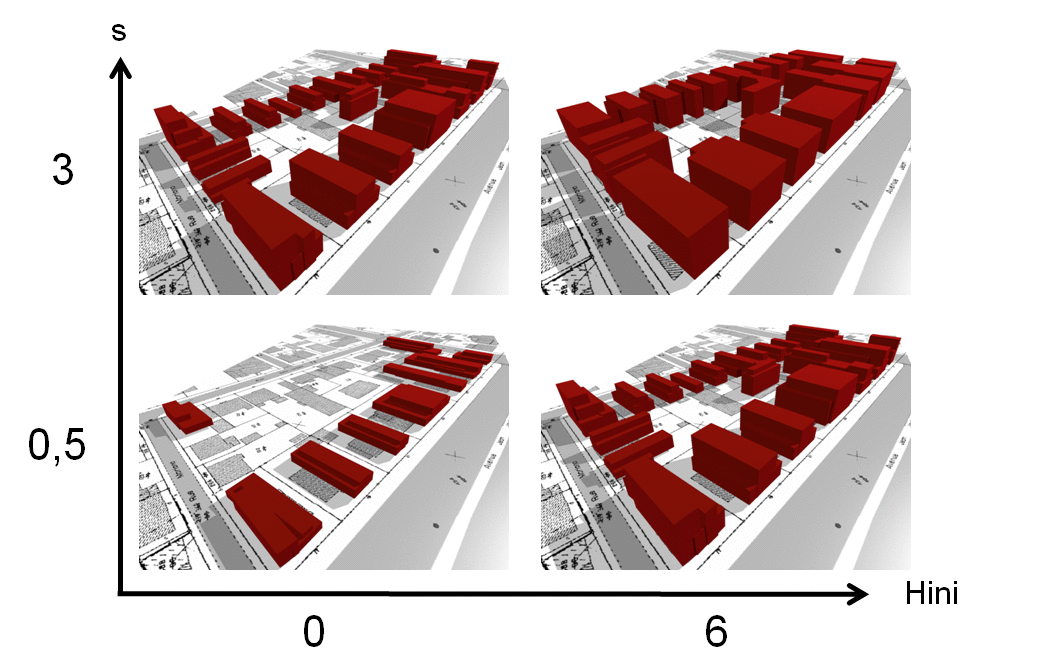
\includegraphics[width=\textwidth]{images/introduction/3d_model_applications/simplu}
                \caption[
                    Example of \acrshort*{acr::3d} urban scene simulated based on known urban norms.
                ]{
                    \label{fig::3d_simulation}
                    Example of \gls{acr::3d} urban scene simulated based on known urban norms.
                    Results obtained using the SimPLU3D tool developped by~\textcite{brasebin2017stochastic}.
                    Different parameter values (building surface \(s\) and initial height \(Hini\)) result in different urban scenery.
                    Urban planners can assess the projected urban density of future districts for better decision making.
                    Image taken from the SimPLU3D website\footnotemark.
                }
            \end{figure}
            \begin{figure}[htpb]
                \centering
                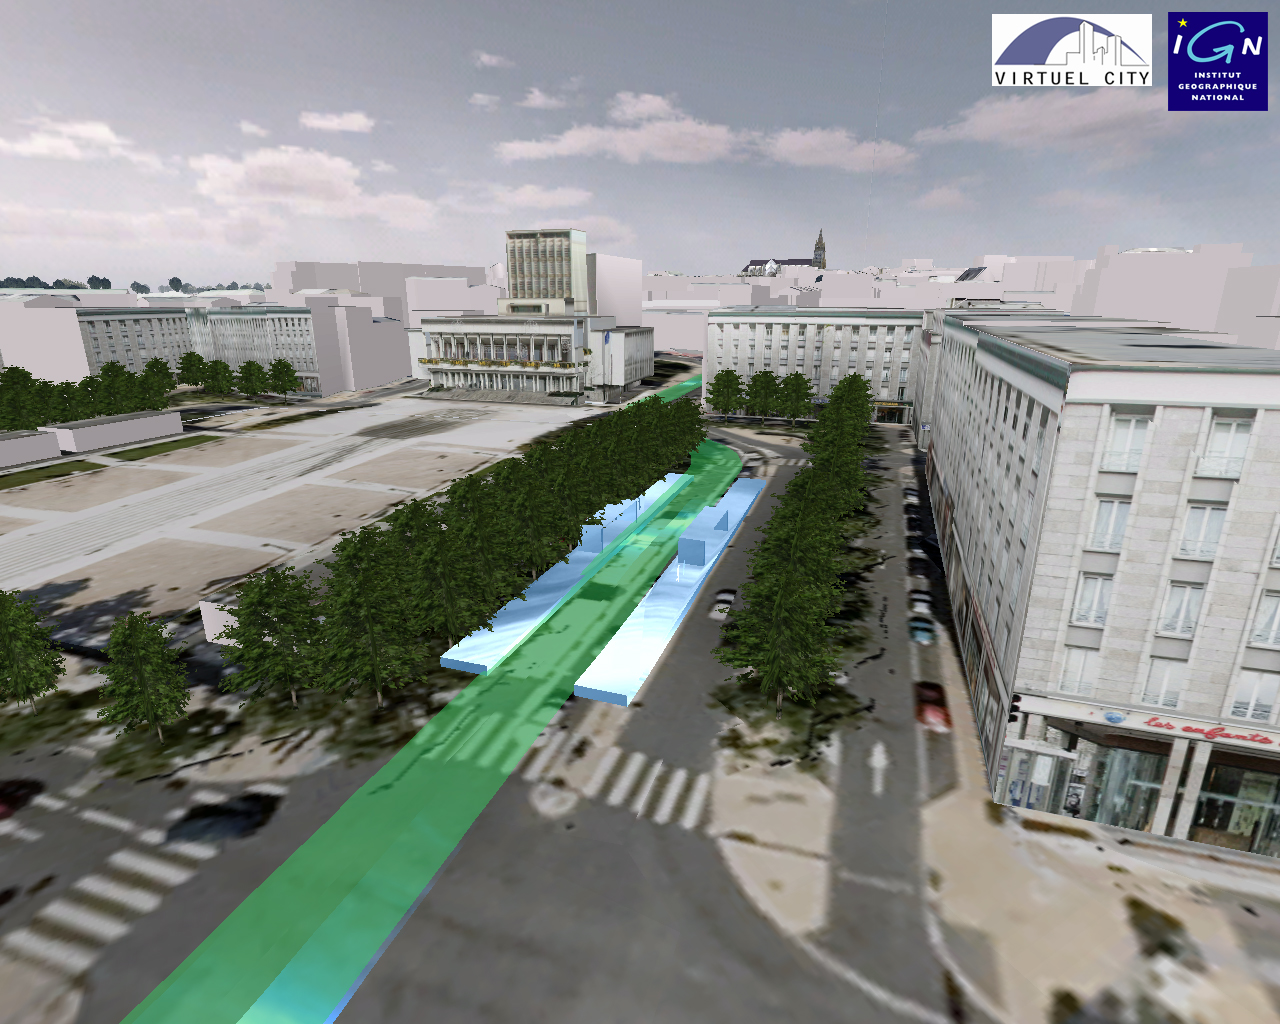
\includegraphics[width=\textwidth]{images/introduction/3d_model_applications/brest_tramway}
                \caption[
                    Example of the use of city \acrshort*{acr::3d} models in public consultation.
                ]{
                    \label{fig::public_consultation}
                    Example of the use of city \gls{acr::3d} models in public consultation.
                    This image was produced using the \gls{acr::ign} Bati3D\textsuperscript{\textregistered} models of Brest, France.
                    The goal is to simulate the impact of the tramway line to be built on the urban landscape.
                }
            \end{figure}

            Related to urban planning, \gls{acr::3d} models could be used as a reference for other planners.
            These models could be used to describe the flow of vehicles and pedestrians in an urban environment as illustrated in~\textcite{vanhoey2017varcity}.
            In addition, it could be used in physical simulations for urban applications.
            For instance, communication companies need to have a \gls{acr::3d} model of urban scenes to predict signal propagation in the goal of optimal network planning~\parencite{yun2007radio}.
            It can be also useful for flood simulation.
            Predicting the height of overflowing water inherently requires a \gls{acr::3d} information.
            This is the usecase of~\textcite{varduhn2015multi}, where \gls{acr::3d} models are used to assess the flood risk.
            Such information could be instrumental for evacuation planning or for insurance managers.
            In the same direction, one can simulate fire propagation~\parencite{dimitropoulos2010fire} or estimating noise propagation in urban scenes~\parencite{stoter20083d} (cf. Figure~\ref{fig::noise_propogation}).

            \begin{figure}[htpb]
                \centering
                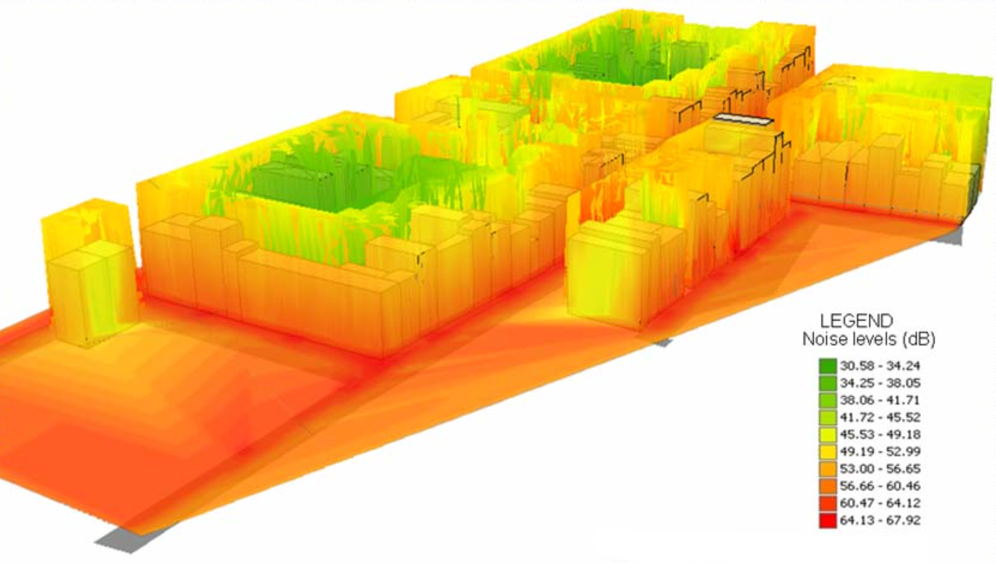
\includegraphics[width=\textwidth]{images/introduction/3d_model_applications/noise_simulation}
                \caption[
                    Example of noise propagation simulation study using \acrshort*{acr::3d} city models.
                ]{
                    \label{fig::noise_propogation}
                    Example of noise propagation simulation study using \gls{acr::3d} city models.
                    Image taken from~\parencite{kurakula2007gis}.
                }
            \end{figure}

            All these simulation derived informations could be supplied to decision makers in order to better plan the cities of tomorrow~\parencite{huck2019urban}.

        \subsubsection{Environmental challenges}
            Environment preservation is a of utter importance in the forecoming years.
            Urban settlement are one of the largest energy consumers.
            A more efficient energy utilization is necessary to sustain the frantic growth of urban areas.
            This motivates the need to quantify the energy consumption of urban settlements~\parencite{WATE20153372} or retrofitting costs~\parencite{previtali2014automatic}.
            \textcite{biljecki2015propagation} also use \gls{acr::3d} models of buildings in order to predict solar irradiation.
            In fact, solar potential estimation can be useful for assessing the benefits of expensive solar panels projects.
            This kind of studies can also be applied in urban planning as the simulations could be undergone for future urban developpements.

            \begin{figure}[htpb]
                \centering
                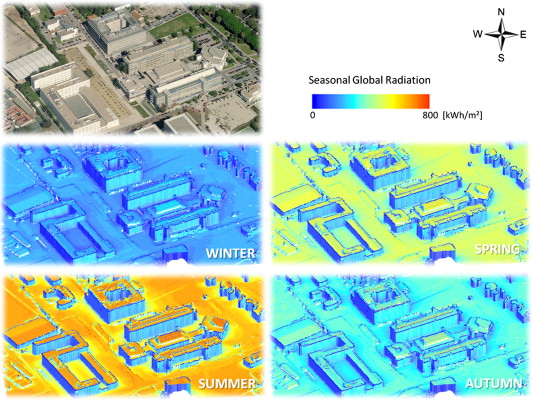
\includegraphics[width=.7\textwidth]{images/introduction/3d_model_applications/solar_potential}
                \caption[
                    Solar potential estimation using building \acrshort*{acr::3d} models.
                ]{
                    \label{fig::solar_potential}
                    Solar potential estimation using building \gls{acr::3d} models.
                    The slope, orientation and dimensions of roofs are determinant factors in computing solar irradiation.
                    Image taken from~\parencite{redweik2013solar}.
                }
            \end{figure}

            Another critical environmental issue that affects cities is air pollution.
            Indeed, it has serious implications on human health as demonstrated in~\textcite{pascal2013assessing} and~\textcite{chen2013evidence}.
            In order to understand its dynamics, researchers simulate the local air flow (i.e., the city microclimate) using computational fluid dynamics.
            This requires a detailed knowledge of the scenes layout.
            One way to acquire this information is through \index{urban!\gls{acr::3d}!model}\gls{acr::3d} models of urban settlements~\parencite{ujang2013unified}.
       
        \subsubsection{Autonomous navigation related challenges}
            Autonomous navigation has seen a great technological leap in recent years.
            Localization is an important step in visual navigation~\parencite{bonin2008visual}.
            \Gls{acr::3d} models play an important role in visual localization~\parencite{biljecki2015applications,piasco2018survey}.\\
            The basic idea is to match an image with a known \gls{acr::3d} model of the city which can be textured or not~\parencite{cham2010estimating,ardeshir2014gis,arth2015instant,christie2016semantics} as shown in Figure~\ref{fig::navigation}.

            % \addtocounter{footnote}{-1}
            \footnotetext{
                \href{https://simplu3d.github.io}{SimPLU3D}.
            }
            \begin{figure}[htpb]
                \centering
                \ffigbox[\FBwidth]{
                    \begin{subfloatrow}[5]
                        \ffigbox[\FBwidth]{
                            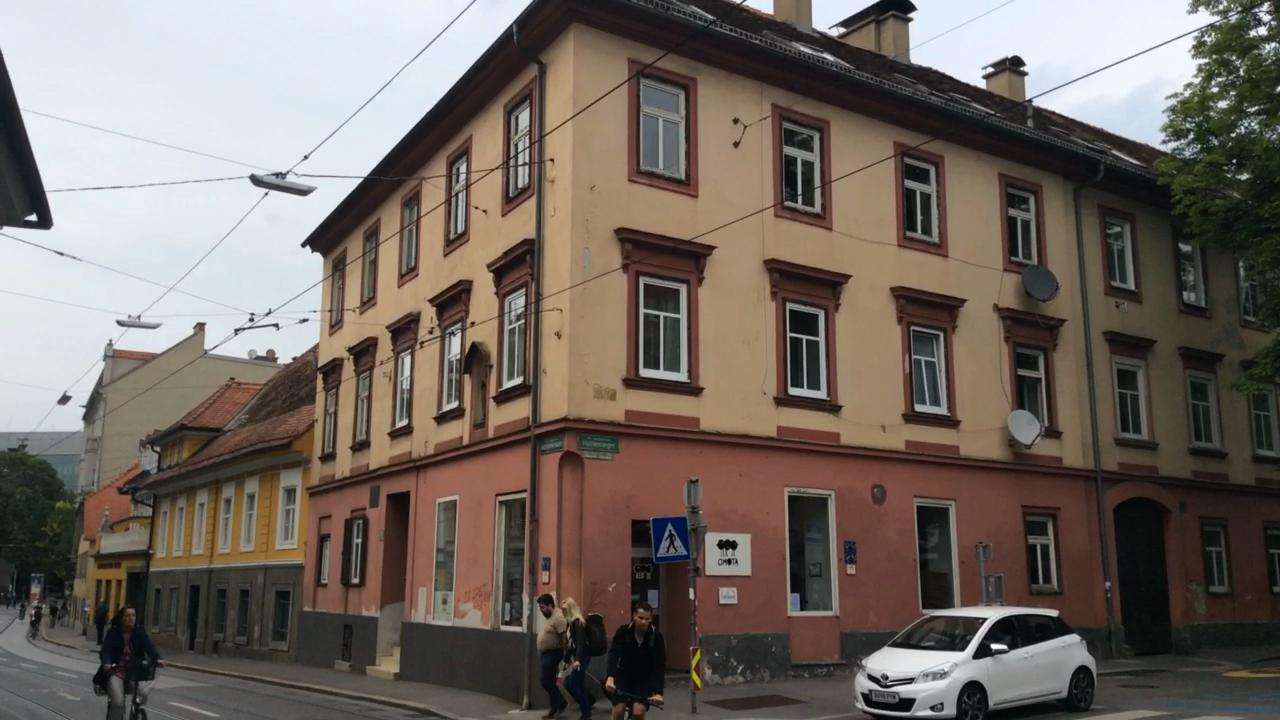
\includegraphics[width=.13\textwidth]{images/introduction/3d_model_applications/pose_estimation/input_image}
                        }{
                            \caption{\label{subfig::input_image} Input image}
                        }
                        \ffigbox[\FBwidth]{
                            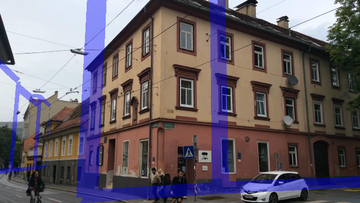
\includegraphics[width=.13\textwidth]{images/introduction/3d_model_applications/pose_estimation/init_pose}
                        }{
                            \caption{\label{subfig::init_pose} Initial estimation}
                        }
                        \ffigbox[\FBwidth]{
                            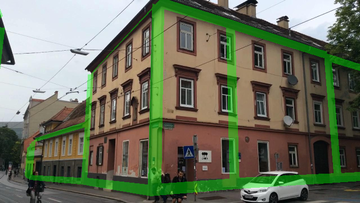
\includegraphics[width=.13\textwidth]{images/introduction/3d_model_applications/pose_estimation/best_pose}
                        }{
                            \caption{\label{subfig::final_pose} Final estimation}
                        }
                        \ffigbox[\FBwidth]{
                            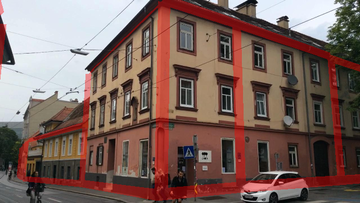
\includegraphics[width=.13\textwidth]{images/introduction/3d_model_applications/pose_estimation/ground_truth}
                        }{
                            \caption{\label{subfig::gt_pose} Ground truth}
                        }
                        \ffigbox[\FBwidth]{
                            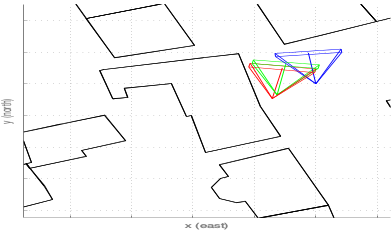
\includegraphics[width=.13\textwidth]{images/introduction/3d_model_applications/pose_estimation/pose_viz}
                        }{
                            \caption{\label{subfig::viz} Different poses.}
                        }
                    \end{subfloatrow}
                }
                {
                    \caption[
                        Position estimation that relies on urban \gls{acr::2d5} models.
                    ]{
                        \label{fig::navigation}
                        Position estimation that relies on urban \gls{acr::2d5} models.
                        The initial pose is derived from a sensor measurement that is not reliable.
                        In Figures~\ref{subfig::init_pose} (\textit{resp.}~\ref{subfig::final_pose} and~\ref{subfig::gt_pose}), the \gls{acr::2d5} model is projected on the image using the initial pose (\textit{resp.} the refined pose and the ground truth one).
                        The \gls{acr::2d5} model helps refine the camera pose.
                        It is shown in the last graph (cf. Figure~\ref{subfig::viz}), where the final estimation (green) is closer to the ground truth (red) than the initial one (blue).
                        Images taken from~\parencite{armagan2017semantic}.
                    }
                }
            \end{figure}

            Once the image matched, one can retrieve an absolute 6-\gls{acr::dog} pose estimation.
            This is especially helpful in urban canyons as shown in~\parencite{piasco2018survey}.\\
            The same ideas can be applied also for indoor environments, such as social cues aware robots navigating alongside humans~\parencite{gupta2018social} or industrial grade robots\addref.
       
        \subsubsection{Entertainement related challenges}
            \gls{acr::3d} models also appeals to various agents in the entertainement industry.
            One of the first examples that comes to mind is the video games community~\parencite{watson2008procedural}.
            In their search for realism, in order to engage the most customers as possible, studios reproduce entire cities as a virtual playing ground for the game story.
            We can cite the "Spider-Man" virtual New-York city\footnote{
                \href{https://www.polygon.com/2013/9/25/4702318/under-the-hood-of-infamous-second-son-hyper-real-seattle}{Under the hood of Infamous: Second Son's hyper-real Seattle}.
            }\footnote{
                \href{https://www.polygon.com/e3/2018/6/12/17453588/spider-man-ps4-new-york-city-avengers-demo-preview}{How Spider-Man PS4’s New York City compares to the real thing}.
            } or the realistic facsimile of Seattle in "Infamous Second Son"\footnote{
                \href{http://www.businessinsider.fr/us/spider-man-ps4-new-york-city-2018-9}{I'm blown away by the virtual New York City of 'Spider-Man' on PlayStation 4 — here's how it compares to the real thing}.
            } as instances of such use.\\
            Tourism can also benefit from such models.
            In fact, virtual touring has become more attainable with works like~\textcite{koutsoudis20073d}.
            For instance, tourists can use such tools to prepare their trip by familiarizing themselves with the city they are visiting.
            This can be possible through mixed or augmented reality as shown by~\textcite{devaux20183d} (cf. Figure~\ref{subfig::augemented_reality}).
            It can also be employed in the service of art.
            Actually,~\textcite{russell2011automatic,aubry2014painting} illustrated how it is possible to align paintings or photographs with \gls{acr::3d} scenes (cf. Figure~\ref{subfig::historical_pose}).\\
            \begin{figure}[htpb]
                \centering
                \ffigbox[\textwidth]{
                    \begin{subfloatrow}
                        \ffigbox[\textwidth]{
                            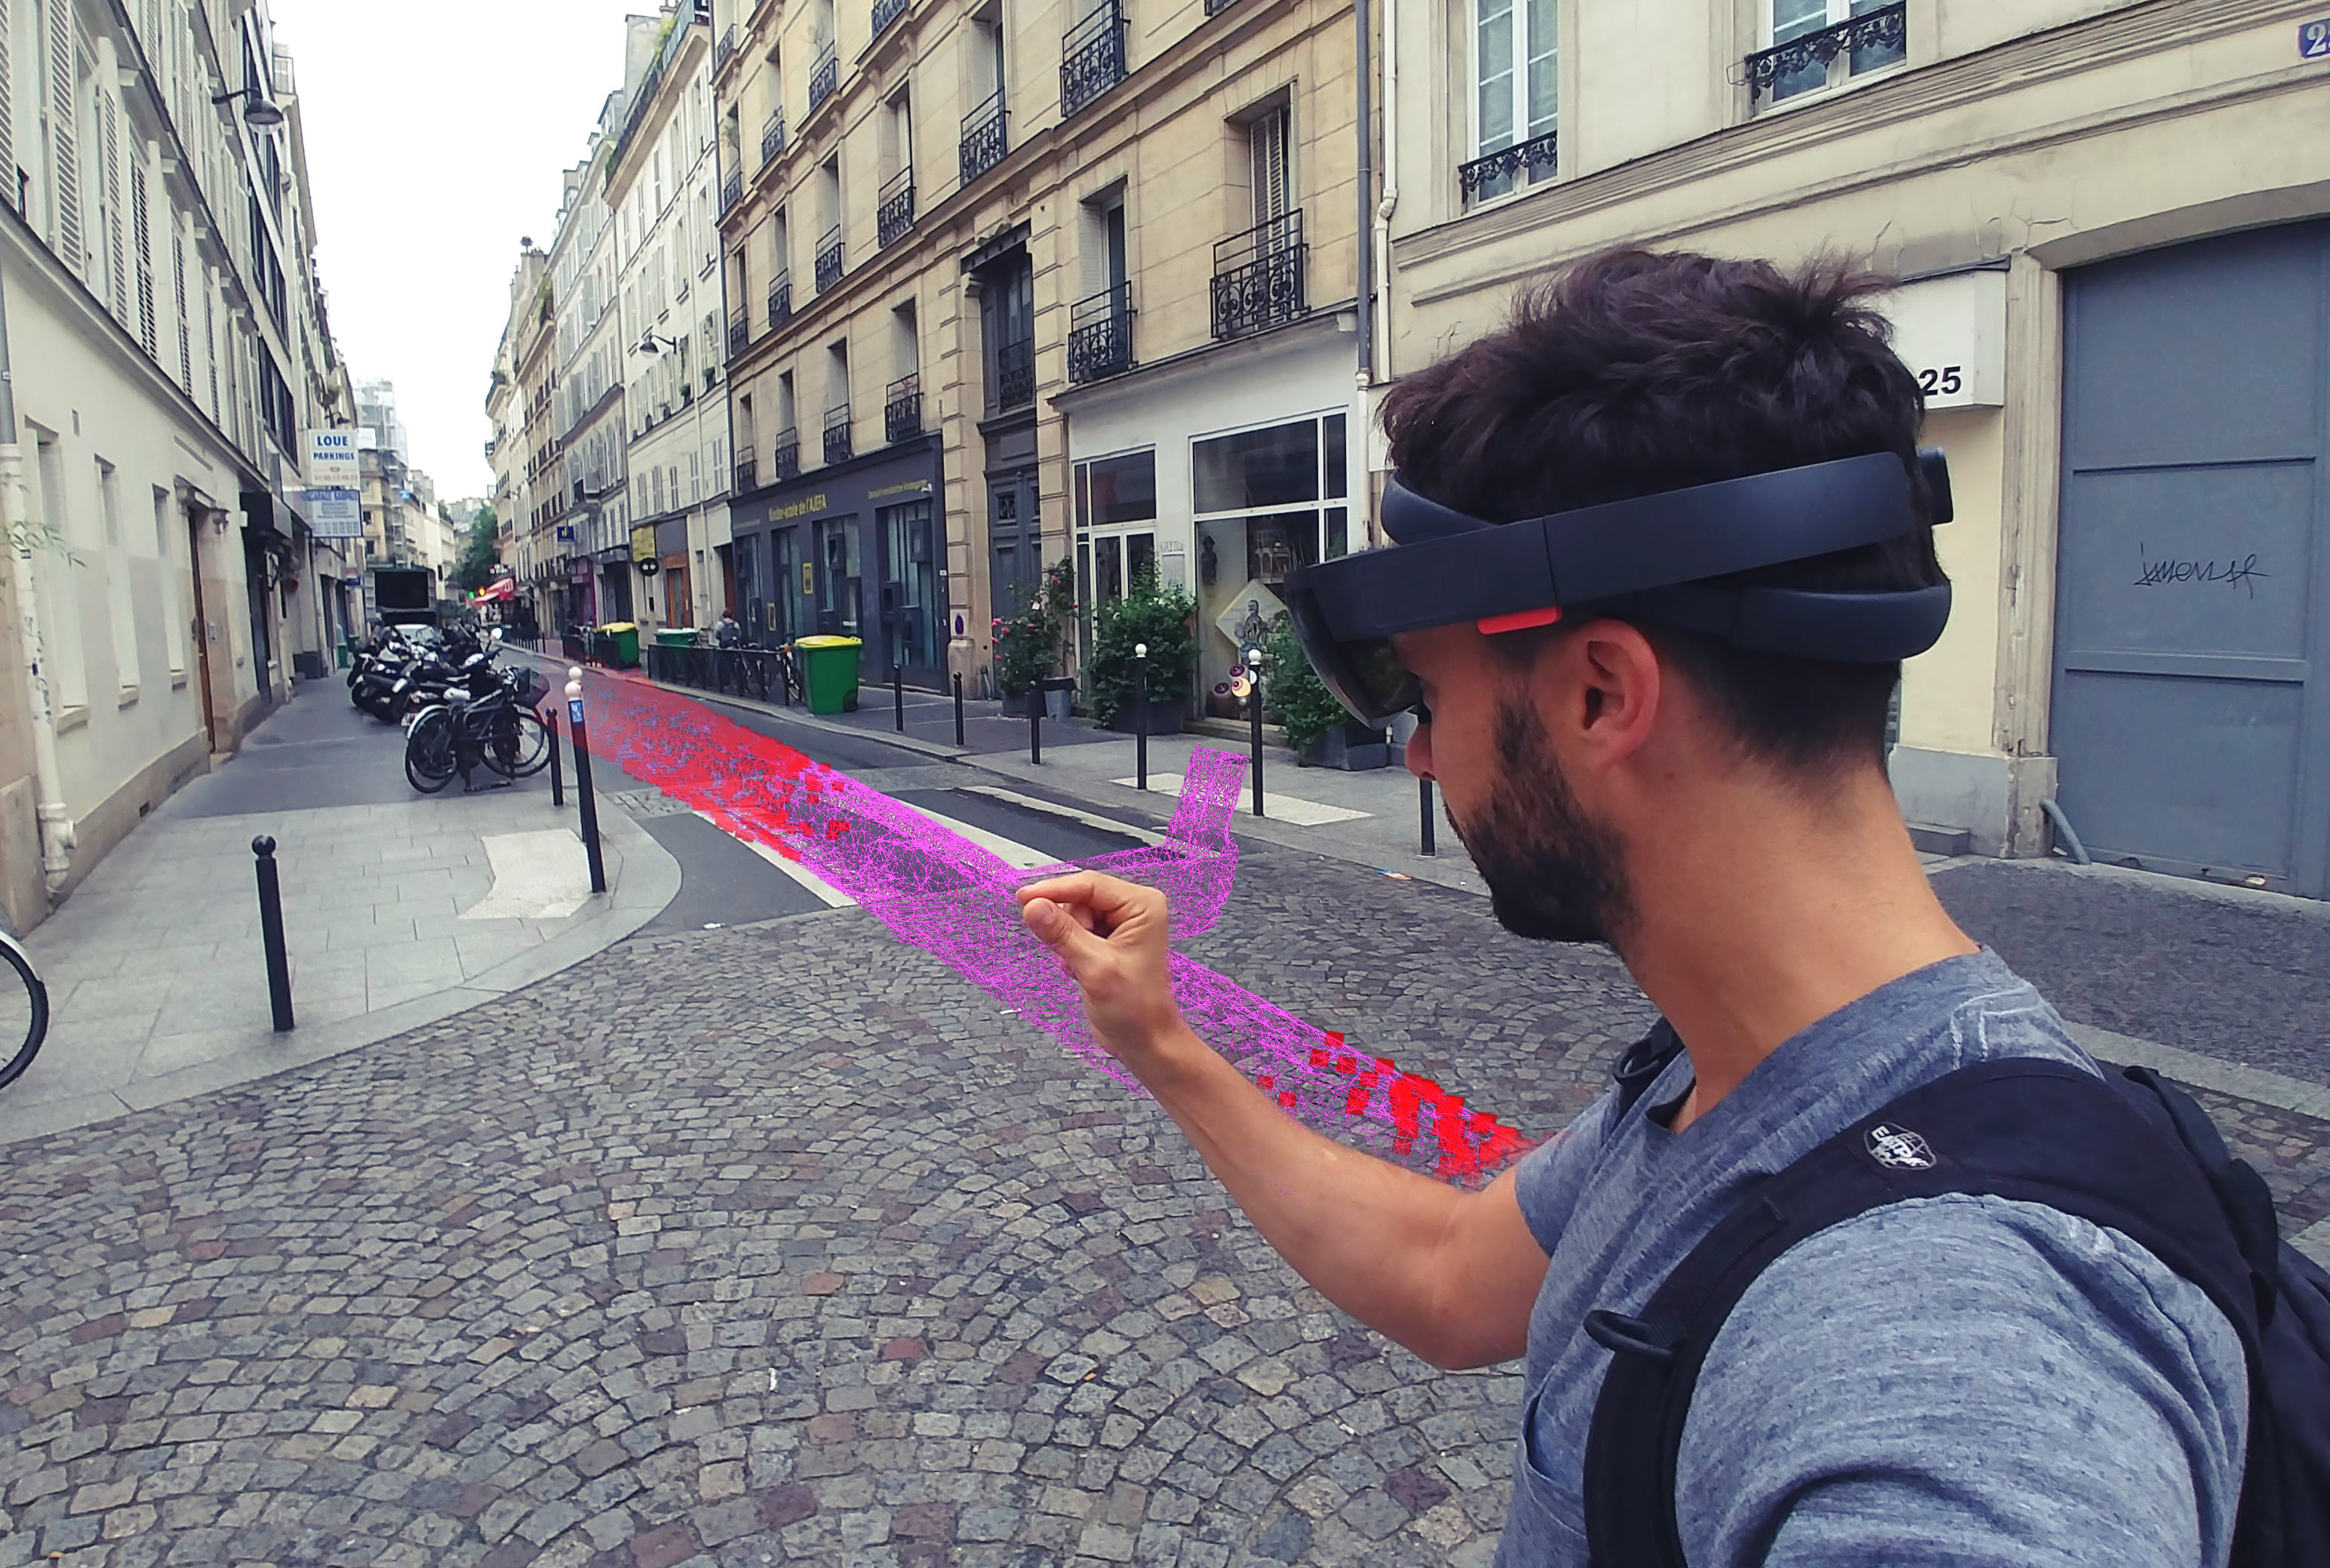
\includegraphics[width=.8\textwidth]{images/introduction/3d_model_applications/insitu_sewer_hololens}
                        }{
                            \caption{\label{subfig::augemented_reality} Virtual vizualization of sewers in Paris based on the \gls{acr::3d} model of the city~\parencite{devaux20183d}.}
                        }
                    \end{subfloatrow}
                    \begin{subfloatrow}
                        \ffigbox[\textwidth]{
                            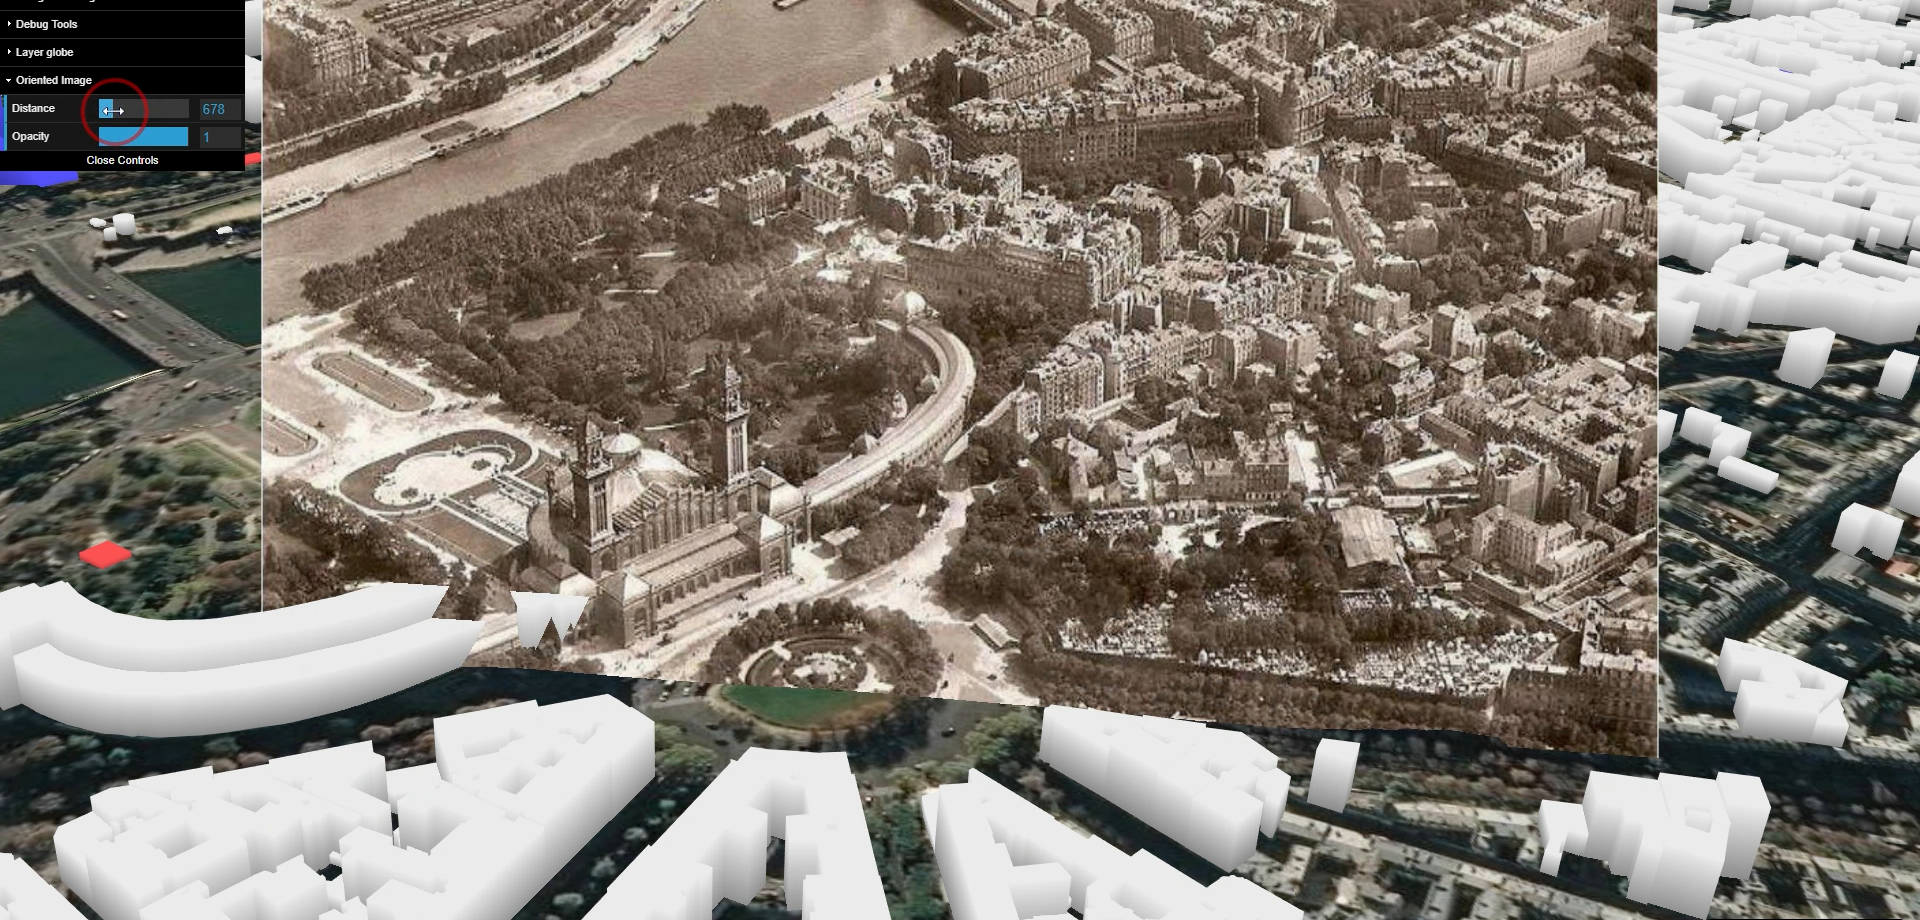
\includegraphics[width=.8\textwidth]{images/introduction/3d_model_applications/trocadero_historical}
                        }{
                            \caption[
                                Pose estimation of a historical aerial image of Trocadero square (Paris, France) that was registered~\parencite{harrach2019interactive} to a city \gls{acr::3d} model visualized with iTowns~\parencite{devaux2012web}.
                            ]{
                                \label{subfig::historical_pose} Pose estimation of a historical aerial image of Trocadero square (Paris, France) that was registered~\parencite{harrach2019interactive} to a city \gls{acr::3d} model visualized with iTowns\footnotemark~\parencite{devaux2012web}.
                            }
                        }
                    \end{subfloatrow}
                }{
                    \caption[
                        Examples of \acrshort*{acr::3d} model applications in the entertainement field
                    ]{
                        \label{fig::entertainement}
                        Examples of \gls{acr::3d} model applications in the entertainement field.
                        Images are courtesy of Alexandre Devaux\footnotemark.
                    }
                }
            \end{figure}

            This last work could be also used to help marketers sell living units.
            Indeed, customers can, for example, visit a digitally reconstructed apartment and virtually furnish it~\parencite{kim2019planar}.
            Another application is living unit pricing.
            In fact, one would not have to travel to the asset location in order to assess it.
            Markerters can do so using its \gls{acr::3d} model.
            For instance, one of the determining factors in estimating buildings is the fa\c{c}ade visibility.
            The latter can be simply measured using building models, as shown by~\textcite{albrecht2013assessing}.

        \subsubsection{Security related challenges}
            Security and emergency fields are not the exception, when it comes to the utilization of city \gls{acr::3d} models~\parencite{kwan2005emergency, ruppel2011designing}.
            For instance,~\textcite{chen2014application} shows how these models are used for ladder trucks optimal deployement planning by firefighters.
            \gls{acr::3d} city models can also be used to determine safe margins in the case of bomb disposal operations.
            This can be possible through explosion simulation in the urban environment of interest~\parencite{willenborg2015simulation}.\\
            \begin{figure}[htpb]
                \centering
                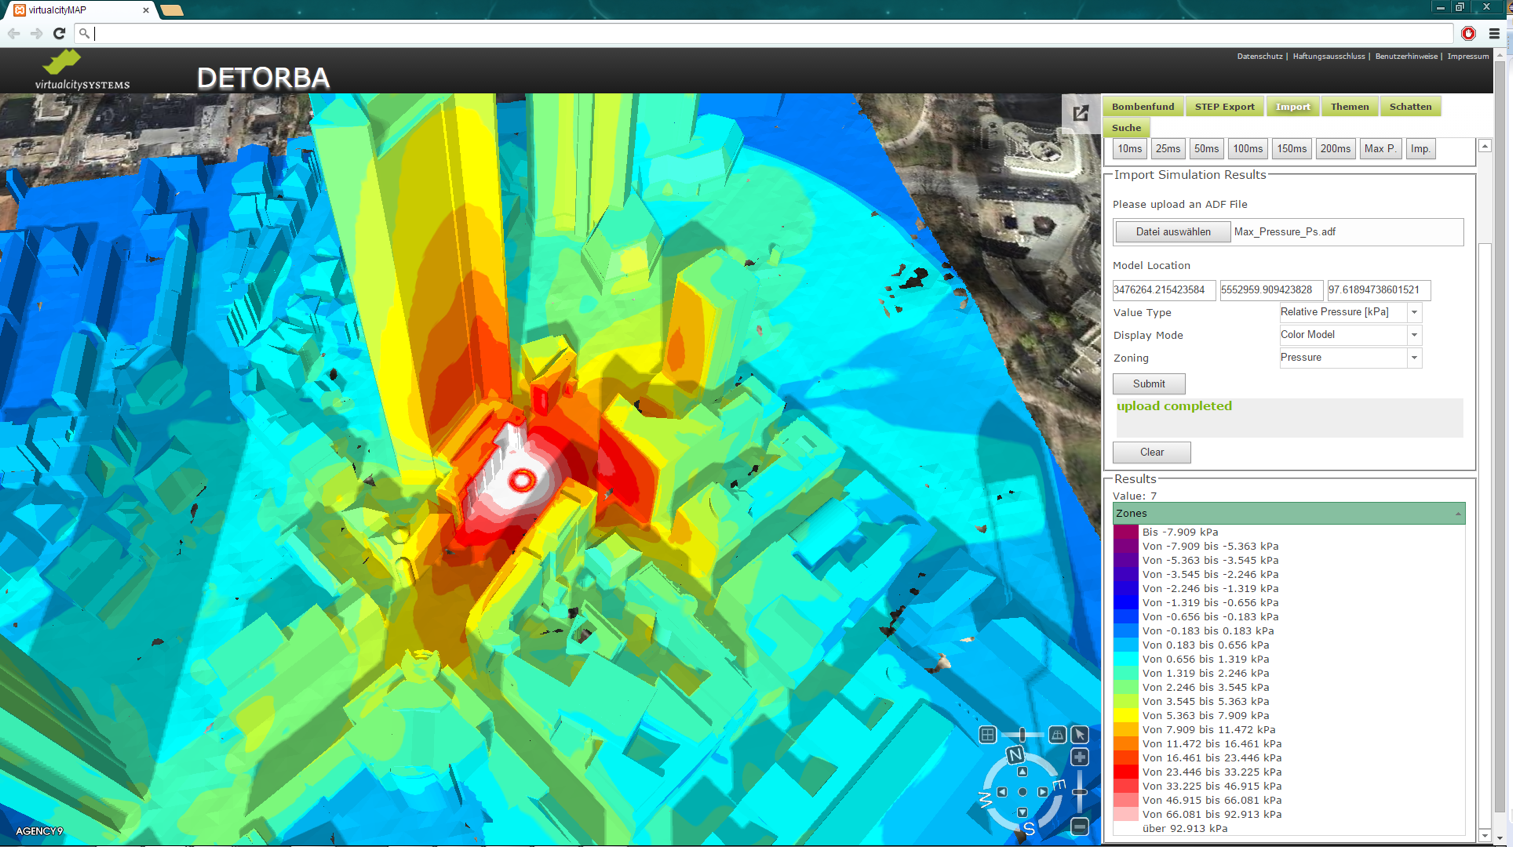
\includegraphics[width=\textwidth]{images/introduction/3d_model_applications/explosion_simulation}            
                \caption[
                    Explosion simulation in urban environments using \acrshort*{acr::3d} building models.
                ]{
                    \label{fig::explosion_simulation}
                    Explosion simulation in urban environments using \gls{acr::3d} building models.
                    Image taken from~\parencite{biljecki2015applications}.
                }
            \end{figure}
            Security forces can equally benefit from city \gls{acr::3d} modeling.
            \gls{acr::3d} models can be used to help analysing crime scenes~\parencite{wolff2009towards}, as well as it can also be helpful for crime prevention as proved by~\textcite{wolff2008geospatial}.
            These models could be instrumental in military applications~\textcite{zlatanova2002trends, budroni2010automatic}.
            Military forces could, indeed, use building \gls{acr::3d} model based augmented reality to train for intervention scenarii, such as hostage rescue operations.

    \subsection{\texorpdfstring{\gls*{acr::3d}}{3D} building modeling}
        \label{subsec::introduction::urban_3d_reconstruction::building_3d_modeling}
        We have seen, previously, how city \gls{acr::3d} models can be instrumental.
        They have a large range of applications in entertainement, industry, security, urbanization and sustainable developpement.
        In this work, the focus is put on outdoor, rather than indoor, modeling.\\

        \addtocounter{footnote}{-1}
        \footnotetext{
            \href{http://www.itowns-project.org}{iTowns project.}
        }
        \addtocounter{footnote}{1}
        \footnotetext{
            \href{http://recherche.ign.fr/labos/matis/~devaux}{Alexandre Devaux website.}
        }

    Precisely, we will raise, herein, the issue of large-scale outdoor city modeling.
        We will see how building reconstruction has a prominent role in the field.
        Afterwhat, we will discuss different building model acquisition techniques and how it influences their quality.
        We end with an examination of semantics in building models.

        \subsubsection{Large-scale outdoor city modeling}
            Not all urban items have the same importance.
            This is particularly true when modeling city scapes.
            For this purpose, all different urban elements are analysed based on temporal and spatial dimensions.
            First, urban elements are clustered into different groups depending on how fast they undergo change.
            \gls{acr::3d} modeling is discussed depending on this mentionned categorization.
            Afterwhat, the spatial differentiation would be used to explain how buildings concentrate the most interest in urban \gls{acr::3d} modeling.\\

            Urban environments are temporally dynamic in nature~\parencite{vanhoey2017varcity}.
            However, constituent items do not evolve with uniform speed.
            Therefore, urban objects are distinguished depending on their change rate.
            Pedestrians --- as well as all living animals in general --- and transportation vehicles are in perpetual movement.
            Water bodies and vegetation, in urban scenes, evolve with an annual or seasonal period.
            Last comes city furniture, roads, bridges, buildings and terrain which have a much lower change frequency.
            We proceed, herein, to study how each of these three groups are modeled in \gls{acr::3d}.\\

            Besides technical difficulties, there are ethical and legal issues when reconstructing \gls{acr::3d} models of humans and vehicles.
            Indeed, accurate reconstruction involves person indentification.
            This has proven to be an intricate subject, as shown by~\textcite{thornton2010individual,tavani2011ethics}.
            Adding to the previous discussion about the high temporal frequency of such objects, seeking the most faithfull models proves to be superfluous.
            In fact, one can populate city models by generic \gls{acr::cad} models of these humans~\parencite{shao2007autonomous} and vehicles.
            Even more so, a lot of aspects of human/vehicle and city interactions do not require \gls{acr::3d} modeling.
            For instance,~\textcite{lovaas1994modeling} can simulate pedestrian traffic flow, which is inherently a \gls{acr::2d} problem\footnote{
                We can safely assume that human do not fly in 2019.
            }, without requiring \gls{acr::3d} human models.\\
            There is little or no work, as far as we know, that discusses \gls{acr::3d} modeling water body situated in urban areas.
            Vegetation can be modeled accurately using \gls{acr::lidar} acquisition~\parencite{omasa20063d}.
            It is, however, too demanding in ressources and unnecessary in a large-scale context.
            Trees are usually modeled by template matching, such as the ellipsoidal form model in~\textcite{lafarge2012creating}, or by generic, species dependent, \gls{acr::cad} models like in~\textcite{iovan2008detection}.\\
            \begin{figure}[htpb]
                \centering
                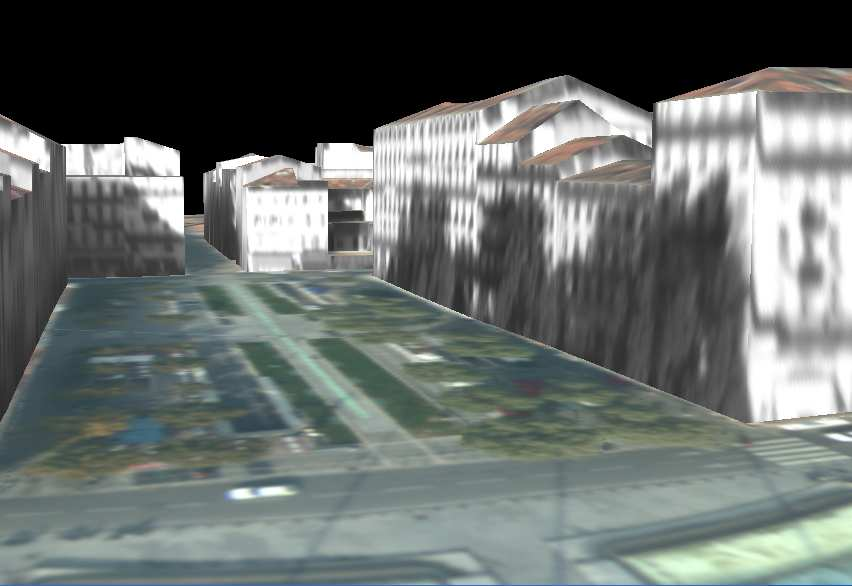
\includegraphics[width=.45\textwidth]{images/introduction/modeling_trees_1}
                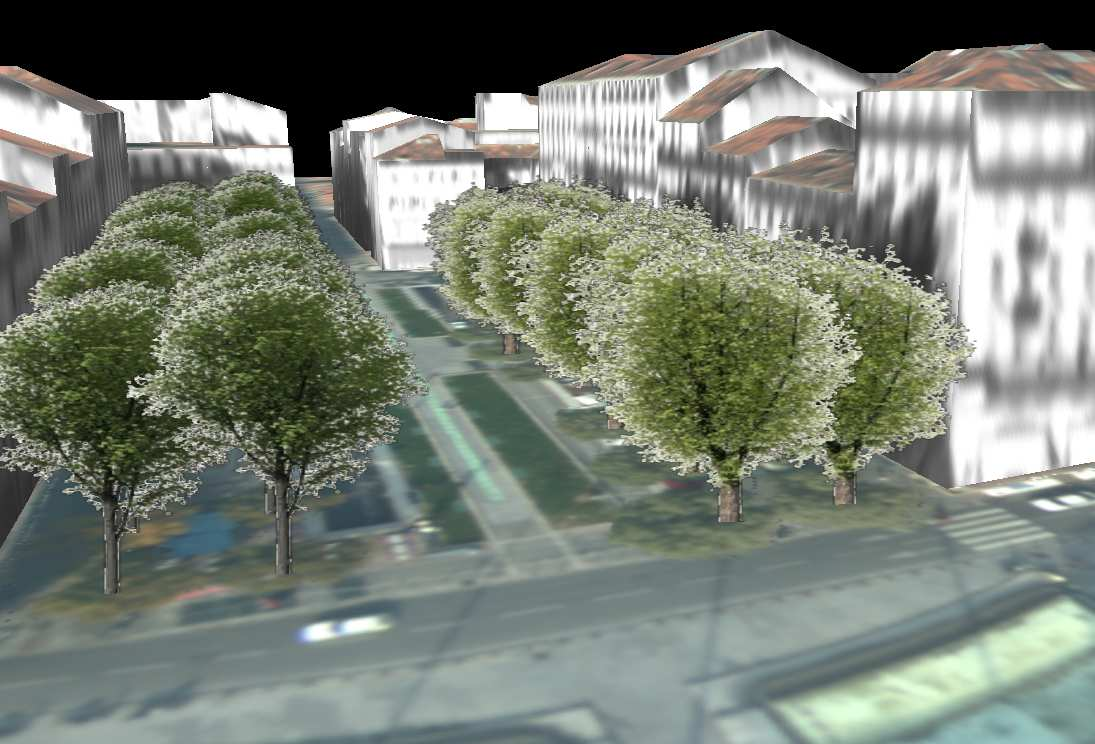
\includegraphics[width=.45\textwidth]{images/introduction/modeling_trees_2}
                \caption[
                    The city model is populated with generic models of trees depending on their class.
                ]{
                    \label{fig::3d_tree_models}
                    The city model is populated with generic models of trees depending on their class.
                    Images taken from~\parencite{iovan2008detection}.
                }
            \end{figure}
            Regarding the first and second groups, was proven, the lack of motivation for precise \gls{acr::3d} reconstruction, in a large-scale setting.
            Exhibiting less temporal volatility, precise modeling of items from the third group seems to be easier.
            In fact, terrain relief can be modeled simply from a \acrfull{acr::dsm} or a \gls{acr::dtm}.
            Although not being so easy to detect~\parencite{mnih2010learning}, roads could be naturally modeled using simple planar structures.
            On the other hand, city furniture, bridges and buildings are more complex.
            While detailed accurate models are needed for buildings and bridges, they are not necessary for city furniture.
            Indeed, it is, for instance, pointless to model each single road sign.
            One would only need to detect its class and reconstruct it, accordingly, using a generic \gls{acr::cad} model portaying the same meaning~\parencite{soheilian2013detection}.\\
            \begin{figure}[htpb]
                \centering
                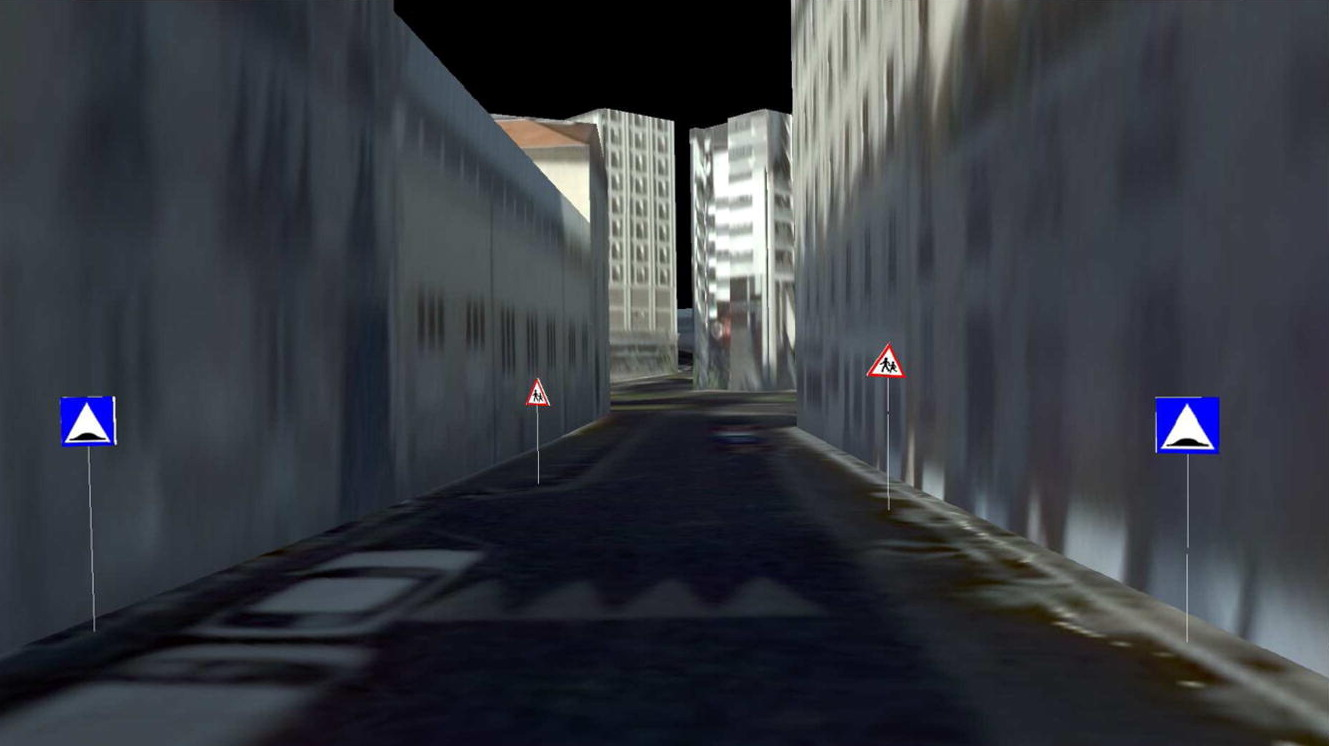
\includegraphics[width=\textwidth]{images/introduction/modeling_road_signs}
                \caption[
                    A city model populated with detected road signs using \acrshort*{acr::cad} models.
                ]{
                    \label{fig::3d_road_signs_models}
                    A city model populated with detected road signs using \gls{acr::cad} models.
                    Image taken from~\parencite{soheilian2013detection}.
                }
            \end{figure}

            Based on the previous temporal frequency differentiation analysis, we narrowed down the urban elements that need special consideration in modeling to two: buildings and bridges. 
            Actually, we can rule out the latter, this time, owing to a spatial frequency study.
            In terms of land cover, the most present objects in an urban environment are roads, vegetation and buildings \addref.
            Hence, modeling these three object types becomes crucial in order to obtain a viable urban \gls{acr::3d} model.
            We have seen previously how roads and vegetation could be satisfactorily reconstructed using relatively simple models.
            This is, however, not the case of buildings.
            That is why, out of all urban features, buildings seem to attract the most attention in urban \gls{acr::3d} modeling.

        \subsubsection{\texorpdfstring{\gls*{acr::3d}}{3D} building modeling}
            Before discussing further on the different types of building models, a definition is provided first.
            A building \gls{acr::3d} model is a cartographic product which represents the surface of the building in question.
            The latter is a generalization of the reality whose goal is not to represent all the details meticulously.
            However, the model should not part from the real geometry of the building of interest.
            Thus, geometric fidelity is weighted against generalization.
            The right compromise is chosen based the final user needs.
            This issue will later intervene often in this work.

            Discussed herein are types of building models.
            Scale of reconstruction is a main factor in dividing the latter into two classes (cf. Figure~\ref{fig::bim_vs_gis}).
            At a small scale, \gls{acr::bim} or \gls{acr::cad} models are easy to use.
            On the contrary, \gls{acr::gis} models are more suitable at a large-scale.\\

            \gls{acr::bim} models are volumetric in nature:
            each element is represented by a volumetric primitive.
            These models are bottom-up: all informations about the building, from the finest details to the most general ones, are aggregated to form the building model.
            A \gls{acr::bim} model is manually constructed as a blueprints of a building before being constructed.
            It has then to follow the buildings evolution in time until its destruction.
            This is the most detailed available virtual representation of a building.\\
            However, it does not come without its own issues.
            First, we can see that it rules out all buildings that predates this convention, especially, historical buildings.
            Secondly, since this type of models require a high interaction with experts, in order to follow the state of the real buildings, it would be almost impossible the fact that the model does not diverge from the reality\addref.
            Third and final, geometric issues, like self-intersections and non 2-manifoldness, affects these models as most \gls{acr::bim} tools do not perform geometric sanity checks.\\

            \begin{figure}[htpb]
                \centering
                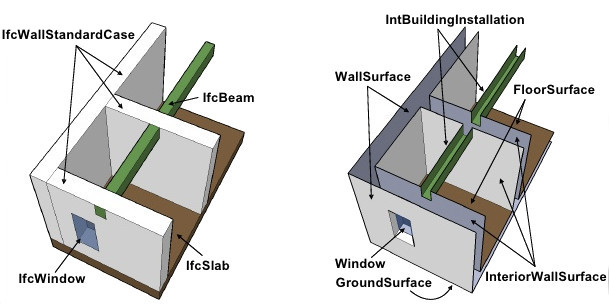
\includegraphics[width=\textwidth]{images/introduction/bim_vs_gis}            
                \caption[
                    \acrshort*{acr::ifc} and CityGML representations of the same object (building storey).
                ]{
                    \label{fig::bim_vs_gis}
                    \gls{acr::ifc} and CityGML representations of the same object (building storey).
                    \gls{acr::bim} (right hand side) is an inherently volumetric model while \gls{acr::gis} (left hand side) represent the surface of the building.
                    Image taken from~\parencite{nagel2009conceptual}.
                }
            \end{figure}

            In contrast, \gls{acr::gis} models represent rather the surface of buildings.
            The goal is to describe the building geometry, as well as all urban items, at a large-scale.
            Furthermore, this model type carries semantics related to all urban objects in the scene as well as their relations.
            These models could be acquired manually, as with \gls{acr::bim}, like the example of~\textcite{ref3dnat}.
            Another way to proceed consists in acquiring the geometry, automatically or interactively, using sensor data~\parencite{musialski2013survey}.
            Crowdsourcing could be equally used for large-scale reconstruction of buildings as depicted in~\textcite{uden2013open}.\\

            Some works tackled the issue of bridging the two model types~\parencite{deng2016mapping}.
            This field is far from being fully mature as proved by~\textcite{stoter2018geo}.
            In addition to the geometric inconsistancies that emanate from \gls{acr::bim} and \gls{acr::gis} model mapping,~\textcite{stoter2018geo} show how semantic ambiguities thwart the automatic conversion from one format to the other.\\

            In this thesis, the scalability\footnote{The capacity of the modeling method to scale at district and even ciy level.} of \gls{acr::3d} modeling is a main concern.
            As a consequence, a special focus is given to automatic and, in a lesser degree, interactive \gls{acr::3d} building modeling techniques.

        \subsubsection{Building \texorpdfstring{\gls*{acr::3d}}{3D} models meets semantics}
            \label{subsubsec::introduction::urban_3d_reconstruction::building_3d_modeling::semantics}
            The surface geometry is not sufficient to describe urban objects~\parencite{biljecki2016improved}, and buildings in particular.
            Semantics are integral part of their representation.
            City models record, for instance, the function of each architectural feature.
            Other informations can be attached to each feature depending on its use.\\
            This kind of information is what is referred to, in this manuscript, as \textit{explicit} semantics.
            The latter has a significant effect on the geometry of the model.
            In fact, architectural elements correspond usually to one or a composite of simple geometric shapes, that are mostly planar~\parencite{kolbe2005citygml}.
            As a consequence, a dense geometric information (i.e., a dense \gls{acr::3d} mesh) is not necessarily the most accurate representation.
            This effect is denoted herein as \textit{implicit} semantics.
            As a consequence, knowing the function of an object helps representing its geometry more efficiently.
            For instance, modeling a column using a cylinder and estimating its radius and height is more accurate than using a non-parametric representation of the same object at a given resolution, while using much less information.
            Hence, semantics implies compaction in the geometric representation of buildings.
            That is why the last criteria was used, for example, in addition to the \gls{acr::rmse}, as an evaluation metric in~\textcite{lafarge2012creating}.\\
            As a consequence, we distinguish, from now on, between a \textit{\gls{acr::3d} model} and a \textit{\gls{acr::3d} mesh} of a building.
            While the latter accounts for the geometric precision, the other conveys, in addition, semantic properties.
            This is illustrated in Figure~\ref{fig::3dmodel_vs_3dmesh}.\\

            \begin{figure}
                \begin{center}
                    \ffigbox{
                       \begin{subfloatrow}
                        \centering
                            \ffigbox[\FBwidth]{
                                \includestandalone[mode=buildnew, width=.7\textwidth]{figures/model_vs_mesh/mesh_model}
                            }{
                                \caption{3D mesh of a building surface ($\approx$ \num{10000} triangles).}
                            }
                       \end{subfloatrow}
                       \begin{subfloatrow}
                        \centering
                            \ffigbox[\FBwidth]{
                                \includestandalone[mode=buildnew, width=.7\textwidth]{figures/model_vs_mesh/ground_truth_model}
                            }{
                                \caption{
                                    Building 3D polyhedral model ($\approx$ 800 facets).
                                }
                            }
                       \end{subfloatrow}
                    }{
                        \caption[
                            Example of the difference between a \acrshort*{acr::3d} mesh compared to a \acrshort*{acr::3d} model.
                        ]{
                            \label{fig::3dmodel_vs_3dmesh}
                            Example of the difference between a \gls{acr::3d} mesh compared to a \gls{acr::3d} model.
                            The first describes only the geometry, while the second is rich in semantics:
                            for each architectural feature corresponds a single geometric primitive.
                        }
                    }
                \end{center}
            \end{figure}
            
            As argued previously, compaction, which results from semantics, is a primordial characteristic of building \gls{acr::3d} models.
            It implies a discretization in generalization levels.
            Indeed,~\textcite{groger2012citygml} uses this property to formalize a discrete and intuitive \gls{acr::lod} scale.
            Even though the original \gls{acr::lod} specification was far from being mature it is widely used in the \gls{acr::gis} and computer vision communities~\parencite{rau2006lod,biljecki2014formalisation}.
            A detailed study of the issue was conducted in~\textcite{biljecki2014formalisation} and ~\textcite{biljecki2016improved}.
            All the same, this work will content itself with the simple intuitive definition of \glspl{acr::lod}.\\
            A \gls*{acr::lod}-0 model corresponds to the \gls{acr::2d5} footprint of the building.
            Next, the \gls*{acr::lod}-1 consists of the \gls*{acr::lod}-0 footprint extruded up to a uniform height.
            \gls*{acr::lod}-2 enhances the previous model scale with more geometrically accurate roof structures.
            The \gls*{acr::lod}-3 reveals even more details, as it models small superstructures, as well as openings.
            Last comes \gls*{acr::lod}-4 which conveys indoor details that are ignored in this work.
            Figure~\ref{fig::lods} depicts these definitions.\\

            \begin{figure}[htpb]
                \centering
                
\includegraphics[width=.7\textwidth]{images/introduction/lods}            
                \caption[
                    \acrshort*{acr::lod} categorization used in this work.
                ]{
                    \label{fig::lods}
                    \gls{acr::lod} categorization used in this work.
                    \gls{acr::lod}-4 is ignored herein.
                    Image taken from~\parencite{biljecki2016improved}.
                }
            \end{figure}
    \subsection{challenges in \texorpdfstring{\gls*{acr::3d}}{3D} building modeling}
        \label{subsec::introduction::urban_3d_reconstruction::challenges}
        The subject of \gls{acr::3d} building modeling has been widely studied in more than twenty years.
        Still, there are some unsolved issues in the field~\parencite{musialski2013survey, lafarge2015some}.
        Presented here is the same classification as in~\textcite{lafarge2015some}.

        \subsubsection{Data acquisition}
            Related to sensor data acquisition are some serious issues, in signal processing in general, just as in \gls{acr::3d} modeling in particular.
            In fact, noise is an integral part of physical measurement processes.
            One should take good care in avoiding error propagation through their processing pipelines.
            For instance, outliers in point-of-interest detection can render a photogrammetrically constructed mesh accumulate sizable geometric errors.\\
            Missing data is also an important issue in \gls{acr::3d}, as some background objects in the scene could easily be occluded by objects in the foreground.
            One way of dealing with this type of obstacles, is to multiply the data acquisition settings.
            This can, actually, help mitigate not only occlusion problems but also noise interference.\\
            However, too much data heterogeneity can also hinder the \gls{acr::3d} modeling process.
            In fact, with more accessible data acquired using different sensors (optical cameras, \gls{acr::radar} and \gls{acr::lidar}, for instance), in various settings (aerial, satellite or terrestrial) and conditions (rainy, sunny, foggy\dots and night-time, day-time\dots), other hurdles need to be overcome.
            For one, more data does not always mean more knowledge, as demonstrated in~\textcite{brachmann2018learning}.
            In fact, one should take good care in choosing how to fuse their input data~\parencite{kedzierski2014terrestrial}.
            For instance, the latter needs be coregistered in the same referential~\parencite{monnier2013registration, mezian2016uncertainty} (cf. Figure~\ref{fig::3d_model_terrestrial_registration}).
            There can also be variabilities in radiometry that needs to be taken into account.\addref
            \begin{figure}[htpb]
                \centering
                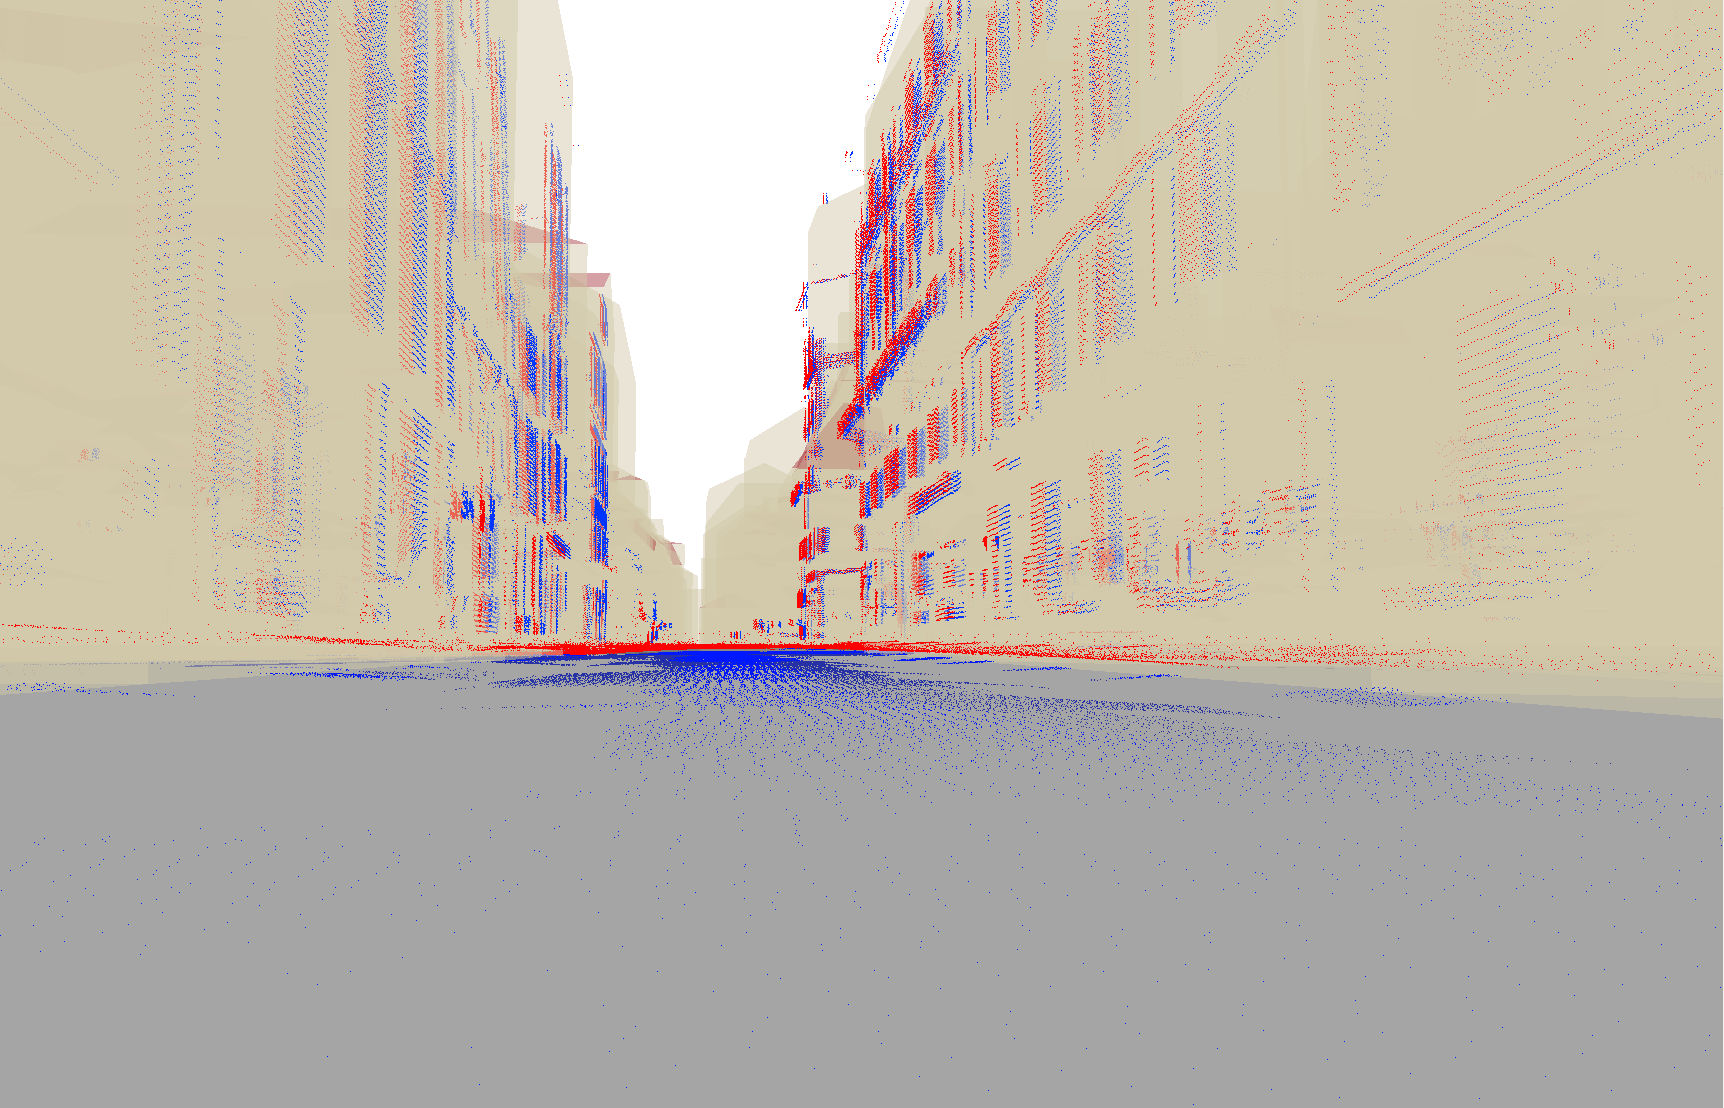
\includegraphics[width=.45\textwidth]{images/introduction/registration_1}
                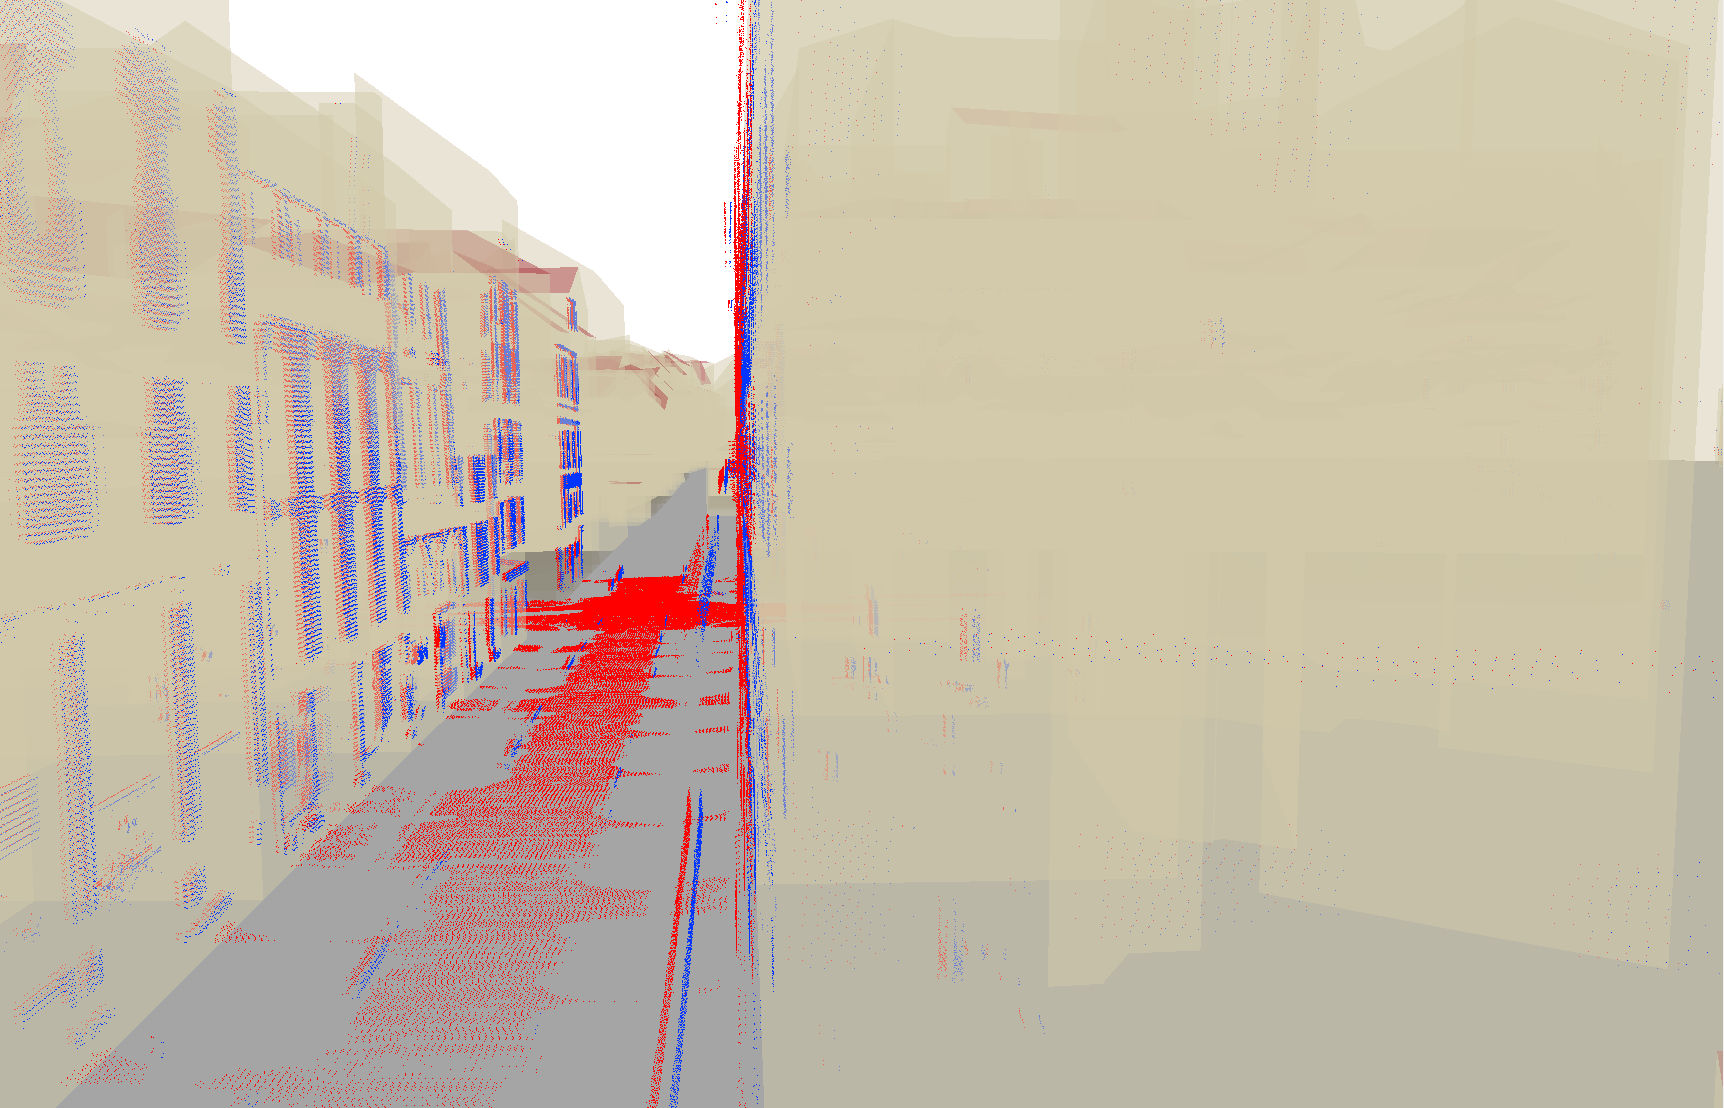
\includegraphics[width=.45\textwidth]{images/introduction/registration_2}
                \caption[
                    Terrestrial \acrshort*{acr::lidar} point clouds are registred against building \acrshort*{acr::3d} models.
                ]{
                    \label{fig::3d_model_terrestrial_registration}
                    Terrestrial \gls{acr::lidar} point clouds are registred against building \gls{acr::3d} models.
                    The registred point clouds can be used to enrich the \gls{acr::3d} models with detailed reconstructions of fa\c{c}ades.
                    In \textcolor{Red}{red}, are represented the raw point cloud while the registred one is illustrated in \textcolor{Blue}{blue}.
                    Image taken from~\parencite{monnier2014}.
                }
            \end{figure}

        \subsubsection{Modeling automation}
            The most accurate approach to produce semantically aware and geometrically accurate representations of a building is a manual one.
            It can be either based on high accuracy \textit{in situ} geodetic measurements (errors are of the order of \SI{0.05}{\m}~\parencite{kaartinen2005accuracy}).
            Although, it is the most accurate representation possible, it is an arduous and expensive process.
            Stereo-plotting consists on using couples of overlapping images in order to manually determine the \gls{acr::3d} geometry of lines.
            It can be used in building modeling to manually plot building edges in \gls{acr::3d} and hence extract its surface.
            This reduces the complexity of the manual modeling process.
            It produces, however, lower precision models as errors are of the order of \SI{0.5}{\m}~\parencite{jamet1995building}.
            This is still a slow process that is highly demanding in terms of operator expertise~\parencite{ruther2002application}.\\
            The manual labour can be alleviated, partly, by automating some parts of the \gls{acr::3d} surface aquisition pipeline~\parencite{musialski2013survey}.
            Some interactive approaches have been proposed to model building.
            The operator is still needed for highly complex semantic tasks~\parencite{mayunga2005semi, castellazzi2015laser}.
            Such methods suffer from imprecision compared to the fully manual ones: for instance,~\textcite{mayunga2005semi} produce models with a geometric error standard deviation in the order of \SI{1}{\m}.\\
            Full automation is still unattainable, especially when it comes to semantics.
            Different strategies are used, where each one targets a specific resolution, balancing between compaction and geometric accuracy.
            Ordered from the most to the least compact, these strategies are listed herein.
            In a Manhattan-world setting, one assumes that buildings are collections of boxes~\parencite{vanegas2010building, li2016manhattan}.
            \textcite{lafarge2012creating, nan2017polyfit} relies on the hypothesis that building are made of piecewise-planar primitives.
            Rich grammars can give rise to less compact but more accurate models, as is the case of~\textcite{demir2015procedural,zeng2018neural}.
            Mesh simplification strategies comes last in terms of compaction~\parencite{zhou20102,verdie2015lod}.
            A sketch of this comparison is presented in Figure~\ref{fig::modeling_strategies}.\\
            \begin{figure}[htpb]
                \centering
                \includestandalone[mode=buildnew, width=\textwidth]{figures/modeling_approaches}            
                \caption[
                    Modeling strategies and the targeted compaction and geometric accuracy.
                ]{
                    \label{fig::modeling_strategies}
                    Modeling strategies and the targeted compaction and geometric accuracy.
                    Depending on the final use of the model, a compromise is chosen between the model compaction and its geometric accuracy.
                }
            \end{figure}
            The compromise, between compaction and geometric precision, relies on an \textit{a priori} knowledge of the modeled urban scene.
            Such hypotheses does not naturally hold at large-scales.
            Multiple factors play a role in architectural styles of buildings that do not always go hand in hand:
            a geographic proximity does not imply always a temporal or architectural closeness for buildings as shown later in Figure~\ref{fig::samples}.
            At a regional or continental scale, the differences become even more overt: cf. Figures~\ref{fig::elancourt_ortho}, ~\ref{fig::nantes_ortho} and~\ref{fig::paris-13_ortho}.
            As a result, some choose to alternate automatic and interactive methods~\parencite{musialski2013survey}: an automatic reconstruction followed by a interactive correction step.
        
        \subsubsection{Quality evaluation}
            As discussed, semantics play a prominent role in building \gls{acr::3d} models.
            Naturally, it should also be taken into account in the evaluation process.
            It is easier said than done.
            Usually, it is indirectly checked using the compaction criterion~\parencite{lafarge2012creating}.\\
            Up to now most studies try to evaluate the quality of modeling algorithms by assessing the accuracy of the geometry of a handfull of buildings.
            These evaluation approaches rely on purely geometric metrics (usually the \gls{acr::rmse}) to compare the reconstructed building to a reference models.
            In a large-scale setting, this becomes prohibitive.
            In fact, it means that one should reconstruct, at least, a whole disctict to be able to judge a city model.
            This is expensive in ressources and time.
            Alternatively, many works favor visual inspection of models.
            This requires, in average, \SI[per-mode=repeated-symbol]{2}{\hour\per\km\squared\per\expert}, and in some cases, is time-consuming  as stereo-plotting the building in the first place.\\
            In the next section, we will discuss, in details, the various ways of evaluating a building model.

\section{Evaluating building models}
    \label{sec::introduction::building_model_evaluation}
    We have just seen how building model quality evaluation is one the main challenges in the field.
    In this section, we present the different types of quality assessement a building model can undergo.
    First, in Section~\ref{subsec::introduction::building_model_evaluation::topological}, is described how models could be checked for their topological consistency.
    On the other hand, the \gls{acr::3d} model geometry has also to be checked against the real building geometry.
    This issue is visited in Section~\ref{subsec::introduction::building_model_evaluation::geometric}.
    Manual geometric inspection is discussed before considering automatic evaluation and its challenges.

    \subsection{Topological consistency inspection}
        \label{subsec::introduction::building_model_evaluation::topological}
        Extensive work has been accomplished in order to achieve a standardized representation of city \gls{acr::3d} models.
        This has resulted in the \gls{acr::ogc} CityGML standard\footnote{\href{https://www.opengeospatial.org/standards/citygml}{CityGML}.}.
        However, in practice, it is not always respected, as shown in~\textcite{biljecki2016most}, where up to \SI{89}{\percent} of models were found to be topologically invalid.\\

        In consequence, the subject of automatic inspection of the topological consistency of city models has drawn a strong attention in the \gls{acr::gis} community.
        The basic common principle is the two-manifoldness of surface representations~\parencite{groger2011achieve}, which aims at excluding self-intersections.
        It is however not sufficient for the complex building cases.
        An urban object, in the international standards is, in reality, represented as an agregation of two-manifold surfaces, as shown in~\textcite{groger2011achieve, ledoux2013validation}.
        This kind of structures can be simply modeled as a \gls{acr::3d} \gls{acr::lcc}~\parencite{damiand2014combinatorial}\footnote{
            An nD \gls{acr::lcc} is an embedding of combinatorial maps in \(\mathbb{R}^n\).
        }, as demonstrated in \textcite{diakite2014topological}.
        This leads to the use of \gls{acr::3d} \glspl{acr::lcc} to check the consistency of city models~\parencite{gorszczyk2016automatic}.
        The idea relies, however, on the presence of reference data to compare to.
        While being very useful for format conversion, sanity checks, as intended in the original paper, are pointless when inspecting \gls{acr::3d} models in the wild.\\
        Not all efforts did fully explore the topological possiblities that are provided by the standard~\parencite{ledoux2013validation,biljecki2016most}.
        In fact, most assume that polygons and solids in the representation are not allowed to have holes, like the work of~\textcite{groger2011achieve, alam2014towards}.
        This was, however, the case of~\textcite{ledoux2013validation}.
        Their work built on the axioms of~\textcite{groger2011achieve}: it does not only deal with polygons and surfaces, but also takes care of solids and allows holes of different dimensions (polygons with holes, surfaces with boundaries\footnote{
            This is actually taken into account by the 2.8D models in~\textcite{groger2011achieve}.
        } and volumes with cavity).
        The errors are organized in increasing order of the geometric dimension of the object they affect.
        The process stops at the dimension of the first detected inconsistancies and ignores the higher ones. 
        An open source library and a web-application are publically available~\parencite{ledoux2018val3dity}, in order to further the sanity of exchanged \gls{acr::3d} models of urban scenes.\\

        We should also mention the efforts made to fix the invalid models. 
        These methods could be divided into local and global ones.
        \begin{description}
            \item[Local approaches:] they rely on local topological operators to solve detected issues in the model.
                    One such method is CityDoctor~\parencite{alam2014towards}.
                    On the downside, these methods have the tendency to introduce more errors in the hope of solving present ones.
                    In fact, the problem is often ill-posed, and multiple solutions can be suggested to alleviate the same problem.
            \item[Global approaches:] the idea is to represent models as volumes constrained by the defectuous surfaces.
                    The goal here, as in urban reconstruction, is to infere topological information from the observed geometric properties, taking into account the unreliability of the data as well as \textit{a priori} information on the model.
                    This is the case of~\textcite{zhao2013automatic}, which relies on a tetrahydralization of the input model volume and a heuristic carving of unnecessary 3-simplices.
                    This approach, in fact, resembles the surface reconstruction procedures from unstructured point clouds using Delaunay triangulation~\parencite{cazals2006delaunay, berger2014state}.
        \end{description}

    \subsection{Geometric inspection}
        \label{subsec::introduction::building_model_evaluation::geometric}
        Guarantying topological consistency is a necessary criterion for the quality of city \gls{acr::3d} models.
        It is, however, not sufficient.
        One would want to assess how close is the building geometry to reality.
        This is what we denote by geometric quality evaluation.\\
        This issue has attracted a lot of attention in \gls{acr::2d}~\parencite{mooney2010towards}, but is not as popular in \gls{acr::3d}.
        This is may be due to the lesser attention that is given to the latter.
        This can be explained by the different levels of difficulty when producing these data.
        It is indeed a more difficult to reconstruct a \gls{acr::3d} model of a building than detecting their footprint.
        For example, one can take a look in the number of submission for each task of the proposed \gls{acr::isprs} benchmark~\parencite{rottensteiner2012isprs, rottensteiner2014results}.
        The \gls{acr::3d} reconstruction task received less submissions than the other one.\\
        Two ways can be used to judge the quality of the geometric representation of a building.
        Manual evaluation relies on human interaction to determine how close the model is to reality.
        The automatic approach relies only on the model and other external data to do so without involving a human in the loop.
        Both are discussed herein.

        \subsubsection{Manual evalutation}
            Manual inspection involves a human operator checking the validity of the reconstructed geometry compared to a reference data.
            The latter could be classified into two types:
            \begin{description}
                \item[Reference building \gls{acr::3d} models:] These are high quality models that were manually produced.
                    One approach is to acquire these on the field by topographic survey.
                    This is, nevertheless, very expensive.
                    Another alternative is to use stereoplotted models using oriented images.
                    This is a more affordable and scalable but a less accurate solution.
                \item[Reference sensor data:] They are used by operators in constrast with what is examined the geometry of a building model.
                    Oriented images, \gls{acr::dsm} and point clouds are instances of such data.
                    This setting is, with the same or less positional accuracy as the previous case, the easiest to adopt in a large-scale.
            \end{description}

            Manual inspection is, actually, ideal in the sense that humans are naturally most suited to detect semantic flaws in building representation.
            The latter are, however, not so adapted for quantitative comparisons.
            One way to alleviate such difficulties is to provide software tools to help measuring inaccuracies in geometry\addref.\\

            In contrast, the most pressing issue is scalability.
            Manual inspection is indeed a laborious task that requires some kind of expertise in the field, for a reasonable efficiency.
            Humans are also not so infallible when assigned precise repetitive jobs.
            Human involvement in the reconstruction effort is especially one of the reasons behind topological inconsistancies in \gls{acr::3d} models.

        \subsubsection{Automatic evalutation}
            In order to achieve scalability, the get-go solution is automation, or failing that, semi-automation.
            As usual, it is easier said than done.\\

            Methods have been proposed to automatically assess building model geometry.
            They rely, however, on ratios that describe the global quality of the model compared to a reference data.
            The flaws are twofold in this case.
            First, global ratios do not capture the finer details in the building.
            Secondly, reference \gls{acr::3d} models are not cheap to acquire, as discussed earlier.
            While the first issue is a manageable issue, as proven in~\textcite{rottensteiner2012isprs}, the second is not so easy to mitigate.\\

            The most crucial problem is, in constrast, the semantic aspect of the quality assessement.
            As discussed, the models in question possess high semantic properties that have a significant effect on their geometry.
            Assessing one without the other is fundamentally unsound.
            While this is easy to achieve manually, it has yet to be incorporated in automatic settings.
\section{Contributions}
    \label{sec::introduction::contributions}
    Based on all the previous discussions, we adopted a research direction that has rarely been taken up to now, as far as we know.
    Our aim is to evaluate the quality of building \gls{acr::3d} models automatically and at large scales.\\

    Herein is explained the path that led to this subject.
    To do so, the context of this work is explained in detail in Section~\ref{subsec::introduction::contributions::positioning}.
    Further on, promising and conceivable utilizations are stated in Section~\ref{subsec::introduction::contributions::use}.
    This is before ending with a summary of the main contributions of this work (cf. Section~\ref{sec::introduction::contributions::contributions}).
    
    \subsection{Positioning}
        \label{subsec::introduction::contributions::positioning}
        As seen in the previous section (\textit{ie.} Section~\ref{sec::introduction::building_model_evaluation}), geometric evaluation of building \gls{acr::3d} models remains a field open for investigation.
        Topologic consistency inspection, in contrast, as discussed in Section~\ref{subsec::introduction::building_model_evaluation::topological}, has received ample attention from the \gls{acr::gis} community.
        In consequence, it will not be of the focus in this work.\\

        Building modeling has been shown, earlier (cf. Section~\ref{subsec::introduction::urban_3d_reconstruction::building_3d_modeling}), to be a bottleneck for urban outdoor modeling at large-scales.
        As a consequence, evaluating building \gls{acr::3d} models is essential for entire scene model inspection.
        Semantics play a prominent role for building models (cf. Section~\ref{subsec::introduction::urban_3d_reconstruction::building_3d_modeling}).
        Geometric fidelity metrics are sufficient in order to faithfully capture the structural properties induced by semantics.
        As a consequence, the proposed approach should factor semantics in the evaluation as well.
        As a result, like with \glspl{acr::lod}, errors are expected to be categorized owing to the semantic character of the evaluation.\\

        The evaluation is, herein, studied under two constraints: \textbf{large-scale} and \textbf{automation}.
        Below, consequences of each one are discussed in detail.
        \subsubsection{Large-scale}
            The implications of this constraints are two-pronged.
            Scalability is at odds with both the heterogeneity of building models and the reference data used for evaluation.
            Both aspects are discussed herein.\\

            Due to the \textbf{large-scale} requirement, the proposed categorization must be stable no matter how the treated urban scene change.
            The same robustness is pursued when considering the different \gls{acr::3d} modeling approaches and the heterogenuous sensors behind the evaluated building models.
            As a consequence, the latter come in in all possible \glspl{acr::lod} and are vulnerable to particular defects, depending on the used modeling method and the input data type.
            Having each urban zone or building model type with its own specific error definitions would hinder scaling the defect categorization.
            In fact, this would involve frequent human interactions in order to alleviate possible issues when merging possibly conflicting error classifications.
            Such interventions are always expensive and scale poorly at district, city or country level, let alone the global stage.\\

            Quality evaluation involves the use of reference data against which reconstructed building models are compared.
            In Section~\ref{subsec::state_of_the_art::quality::reference}, are discussed the different forms these data can take.
            A high quality reference usually requires manual labour that is evidently non scalable.
            Actually, the less costly the reference data is, the more adaptive the evaluation method will be at large scales.
            In fact, the best alternative would be, if possible, to avoid using reference data altogether.

        \subsubsection{Automation}
            Semantically aware inspection is a natural task for human operators.
            It is, however, challenging to automate.
            In fact, as seen in Computer Vision, the more semantic tasks are, the more difficult they are to automate.
            It is even more arduous taking into account the \textbf{large-scale} constraint which implies a robustness to the natural heterogeneity in urban scenes as well as the variance of modeling approches.

    \subsection{Application cases}
        \label{subsec::introduction::contributions::use}
        Ahead was discussed the context of the proposed work.
        Hereafter is discussed the potential use of a semantically aware automatic geometry evaluation of building \gls{acr::3d} models.
        \subsubsection{Change detection}
            This is possible in two ways.
            First, one can consider the same approach that is used for error detection as a method for change detection in building \gls{acr::3d} models.
            This is equivalent to considering change as an semantic error that impacts the geometry of the building.
            Second is the fact that change can be implicitly detected from geometric errors.
            In fact, the change that can be observed from sensor data, will render the outdated model invalid geometrically.
            \begin{figure}[htpb]
                \centering
                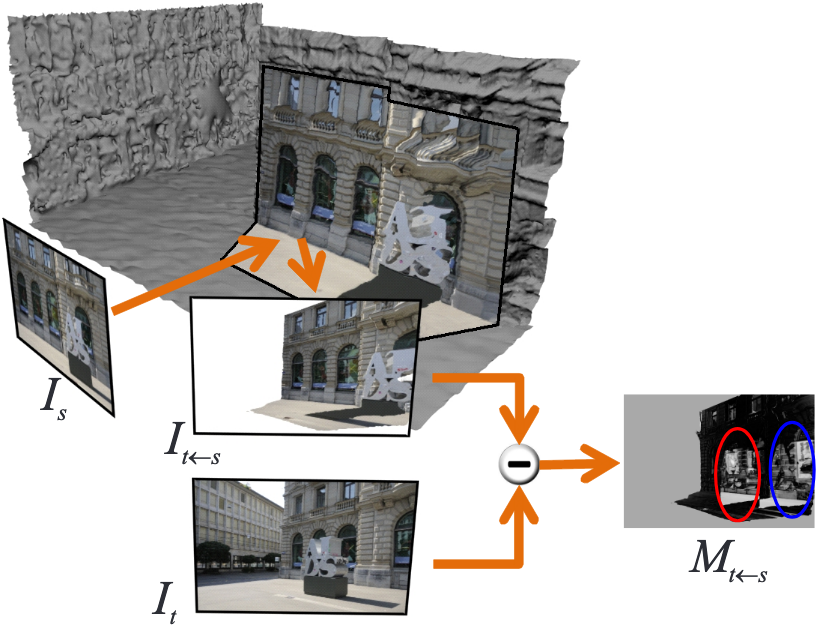
\includegraphics[width=.7\textwidth]{images/introduction/use/change_detection_taneja}
                \caption[
                    Illustration of change detection in urban areas.
                ]{
                    \label{fig::3d_change_detection}
                    Illustration of change detection in urban areas.
                    Image taken from~\parencite{taneja2013city}.
                }
            \end{figure}

        \subsubsection{Building model correction}
            This is the most obvious usecase for this work.
            In practice, errors are detected by operators in order to correct them.
            The first task, if automated, can be time saving in the correction post-processing step.
            It is even possible to automate the whole correction process using the advances achieved in interactive reconstruction~\parencite{kowdle2011active}.
            \begin{figure}[htpb]
                \centering
                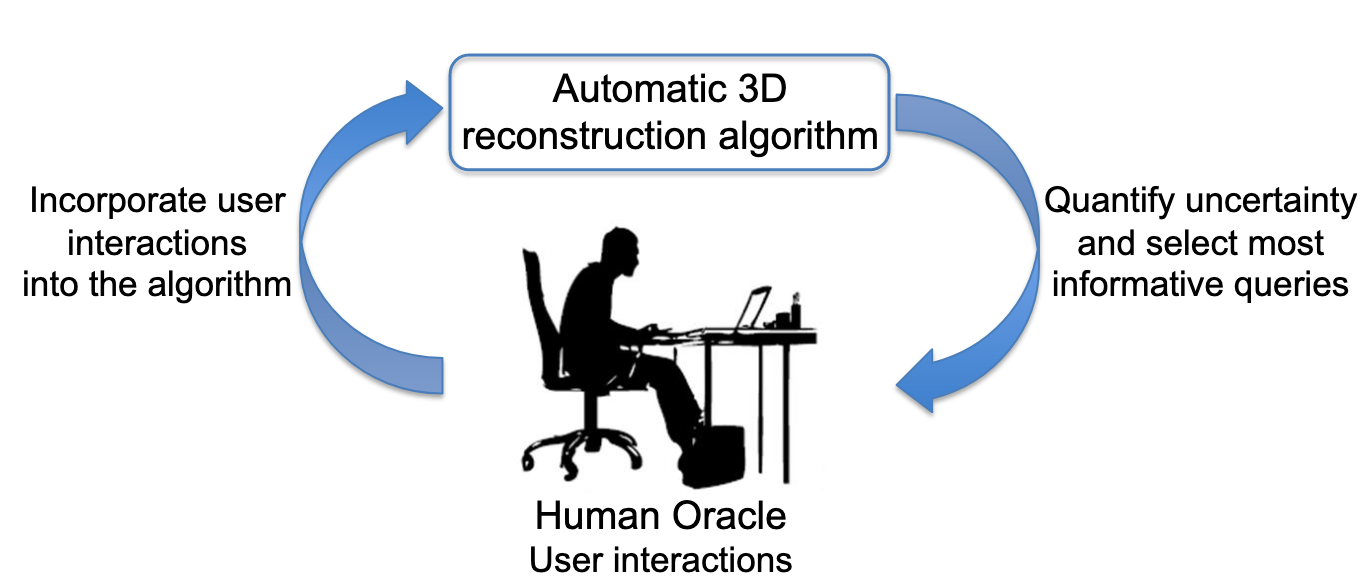
\includegraphics[width=.7\textwidth]{images/introduction/use/active_learning_kowdle}
                \caption[
                    Example of an interactive pipeline that needs human operators to provide correct initial reconstructions.
                ]{
                    \label{fig::corrections}
                    Example of an interactive pipeline that needs human operators to provide correct initial reconstructions.
                    Image taken from~\parencite{kowdle2011active}.
                }
            \end{figure}

        \subsubsection{Reconstruction method selection}
            Evaluation of the building models can help selecting the most adapted reconstruction methods for a certain urban scene.
            Indeed, depending on the needs of the potential final user, some errors are to be watched more than others.
            As an example, an insurance agent, who is only interested in flood simulations, will not be interested by the geometric accuracy of \gls{acr::lod}-2 features and will focus principally at the \gls{acr::lod}-1 representation errors.
            Modeling algorithms are naturally biased towards a given setting that depends on the hypotheses chosen by their creators.
            They will produce less errors when those conjectures are met and fail otherwise.
            These assumptions are fixed, for instance, in terms of building types (Haussmann style, Manhattan-world \dots), geometric criterea (planar surfaces, symmetry \dots).
            Hence, choosing a modeling approach can determine how good are the models and vice versa.
            \begin{figure}[htpb]
                \centering
                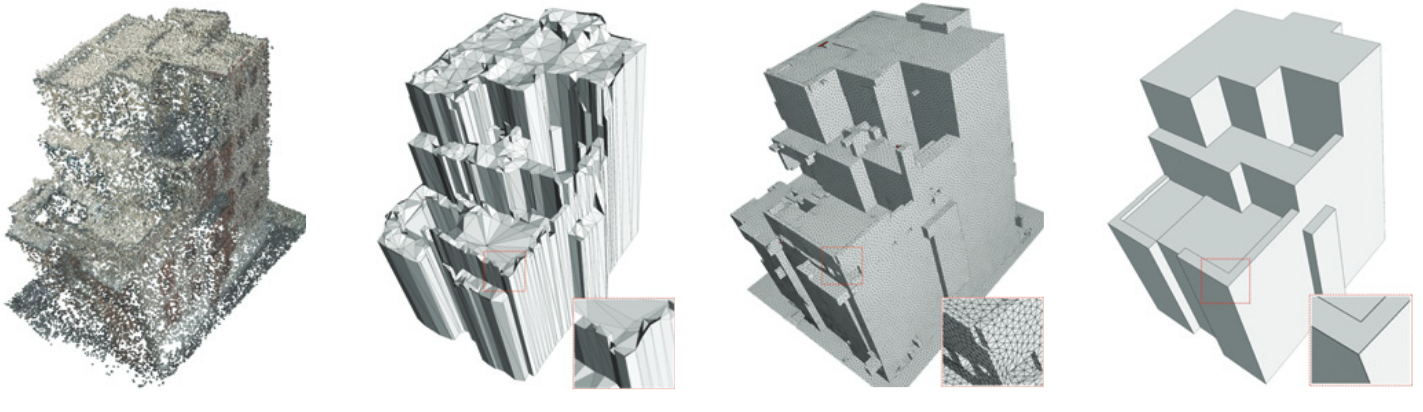
\includegraphics[width=.7\textwidth]{images/introduction/use/comparison_li}
                \caption[
                    Depiction of different models for the same building.
                ]{
                    \label{fig::comparison}
                    Depiction of different models for the same building.
                    Image taken from~\parencite{li2016manhattan}.
                }
            \end{figure}

            \subsubsection{Crowdsourcing evaluating}
            Crowdsourcing~\parencite{kovashka2016crowdsourcing} can be seen as a building modeling method.
            It has become easier with the help of some online tools like SketchUp\footnote{
                \href{https://www.sketchup.com}{SketchUp website}.
            }, where anyone can model, for instance, their home and share it publically.
            The quality of the models depend on their author.
            An automatic evaluation method can help check that the uploaded models respect the specifications.
            Another issue is the presence of vandalism in open data~\parencite{neis2012towards}.
            The presented approach can be used to help understanding user behaviors and detect vandaliser.
            \begin{figure}[htpb]
                \centering
                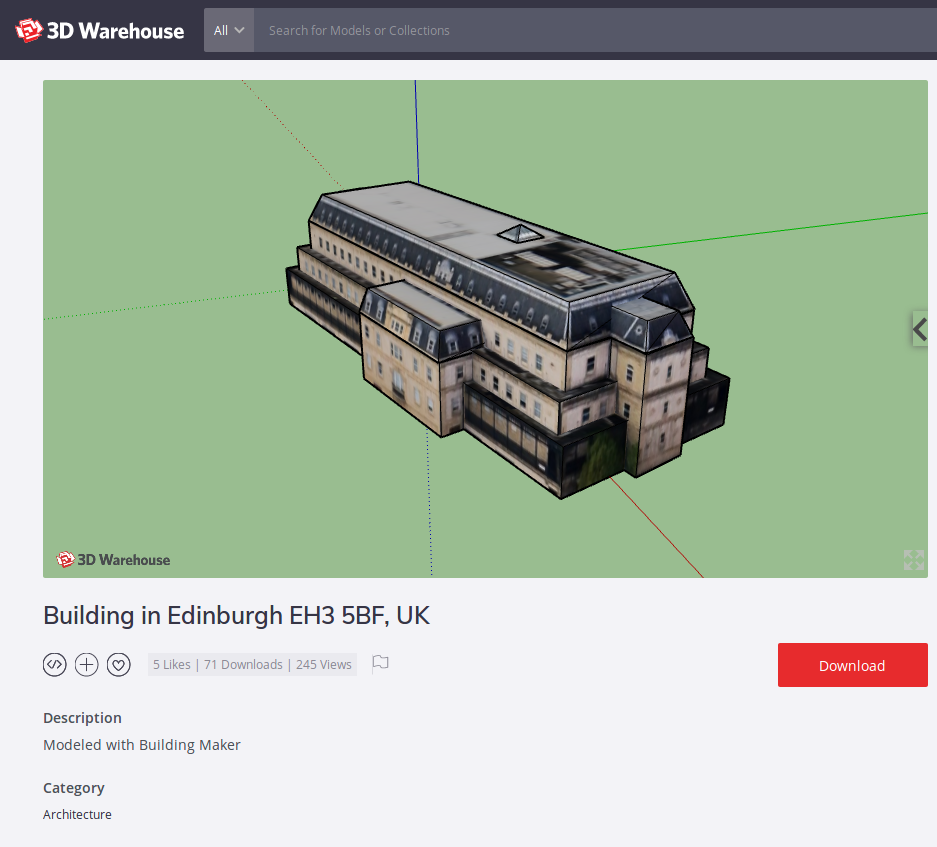
\includegraphics[width=.7\textwidth]{images/introduction/use/crowdsourcing}
                \caption{
                    \label{fig::crowdsourcing}
                    A sample of a building model made by a SketchUp user.
                }
            \end{figure}

    \subsection{Main contributions}
        \label{sec::introduction::contributions::contributions}
        Based on the detailed discussion hereinabove, we present our contributions in the field of geometric evaluation of building \gls{acr::3d} models.
        They are four-fold.
        A graphical abstract is presented in Figure~\ref{fig::graphical_abstract} giving an overview of our contributions.
        \begin{figure}[htpb]
            \centering
            \includestandalone[mode=buildnew, width=\textwidth]{figures/graphical_abstract/graphical_abstract}            
            \caption[
                Our semantic evaluation framework for \acrshort*{acr::3d} building models.
            ]{
                \label{fig::graphical_abstract} Our semantic evaluation framework for \gls{acr::3d} building models (a).
                Semantic errors affecting the building are predicted using a supervised classifier and handcrafted features.
                In addition to the input model topological structure (b), features are extracted from Very High resolution overhead data.
                It can be based on a comparison with the \gls*{acr::dsm} (c).
                Optical images can also be used through, for instance, local gradient extraction (d).
                Several errors can be detected at the same time, in a hierarchical manner (e).
                Fidelity errors correspond to geometrical imprecision as shown in red.
                On the other hand, modeling errors denote morphological inconsistancies with the real object.
            }
        \end{figure}
        \subsubsection{Error taxonomy}
            A hierarchical and adaptive taxonomy of errors is proposed.
            It is designed to be independent from the urban scene or the modeling approach.
            In order to achieve this, errors are chosen meticulously as a compromise between generalization and expressivity.
            The first ensures that errors from the taxonomy can fit any scene, while the second implies that errors are not equivocal.
            It is also an adaptive categorization, since, depending on the final user needs, a set of errors can be extracted after specifying some parameters.
            
        \subsubsection{\texorpdfstring{\gls*{acr::3d}}{3D} model reference free evaluation}
            Acquiring \gls{acr::3d} reference models is very expensive in ressources and particularly not scalable at large-scale.
            As a consequence, the problem is formulated as a supervised learning one.
            Based on the errors, that are extracted from the taxonomy, a classifier is trained in order to predict defects for unseen models.

        \subsubsection{Custom features}
            Since the formulated problem has not been massively studied, there was no feature extraction baseline to compare to.
            Hence, a baseline of features is presented in this work.
            In addition, we also presented some more advanced ones relying on \glspl{acr::scatnet} and graph kernels, with the aim of improving on the detection rates of the baseline approach.
            They are computed based on the geometric attributes of the building model and the comparison to external remote sensing data: \gls{acr::vhr} optical images and height maps.
        
        \subsubsection{Scalability analysis}
            One of the goals of this work is to achieve scalability in large-scale.
            This implies the transferability of the learned predictors to unseen urban settings or untested modeling techniques.
            It involves also a representativeness and generalization study of the training sets.
            An analysis is conducted accordingly.
            We experimentaly prove the stability of classifiers, under some settings.
        
        \subsubsection{\texorpdfstring{\gls*{acr::3d}}{3D} model handling}
            We also developped a set of tools to handle the geometry of \gls{acr::3d} building models.
            They were necessary in order to manage poorly stored models.
            It was also useful in computing exact projections of polyhedral buildings and extracting other useful informations that were later used for feature extraction.

\section{Structure of the Thesis}
    \label{sec::introduction::structure_of_thesis}
    The remainder of the thesis is organized in five main chapters.\\
    \begin{itemize}[label=\(\blacktriangleright\)]
        \item Chapter~\ref{chap::state_of_the_art} provides a global overview on state-of-the-art techniques in fields related to our main subject.
                In fact, in order to have a general idea on the \gls{acr::3d} building modeling domain, we provide a summary and a broad categorization of techniques that can be found in the litterature.
                We also provide a detailed account of all quality evaluation methods that are used by the community.
                Afterwhat, we present a global view of methods from the litterature on supervised classification as well as feature extraction which were instrumental in our approach.
        \item In Chapter~\ref{chap::semantic_evaluation}, we introduce the first leg of our approach.
                It consists in defining a general layout of a \textbf{large-scale} adaptive error taxonomy.
                Applied to the overhead setting, and based on observations of automatically modeled buildings, we implement this layout by defining semantic errors to populate the taxonomy.
        \item \textbf{Automation}, which is the second and remaining constraint defined in Section~\ref{subsec::introduction::contributions::positioning}, is handled in Chapter~\ref{chap::learned_evaluation}.
                Actually, aiming to automate a semantic task, we introduce a learning based approach where errors are treated as labels which are predicted using a trained supervised classifier.
                Features are extracted based on the intrinsic properties of building models as well as extrinsic attributes making use of external optical or depth based data.
        \item This proposed approach is then tested on multiple urban scenes as shown in Chapter~\ref{chap::experiments}.
                The latter provides in depth details about the origin of the evaluated building models as well as the used algorithms.
                The different baseline features are tested on all urban areas yielding mitigated results which depend on the combination of defined errors and urban scenes.
        \item Chapter~\ref{chap::more_experiments} compiles results from multiple experiments that further tests the pipeline.
                To satisfy the already stated \textbf{large-scale} need (cf. Section~\ref{subsec::introduction::contributions::positioning}), a scalability analysis is drawn based on various experiments involving the presented urban zones.
                Next, the framework is tested at a lower specificity level (cf. Section~\ref{sec::semantic_evaluation::general_framework}).
                The choice of classifiers is also discussed based on exhaustive experiments.
                Finally, a thorough testing of advanced features, which take into account the structural information that was missed by the baseline, yielded results that were profusely analysed.
        \item The final Chapter~\ref{chap::conclusion} concludes the thesis by presenting a summary of the proposed approach as well as experimental results to support it.
                Final thoughts on underdiscussed perspectives of research are also adressed.
    \end{itemize}

   
    \chapter{\textsc{State-of-the-art}}
        \label{chap::state_of_the_art}
        \minitoc

\vfill

\clearpage

\section{Automatic building \gls*{acr::3d} modelling}
    \label{sec::state_of_the_art::building_modeling}

    \subsection{Input data classification}
        \label{subsec::state_of_the_art::building_modeling::input}

    \subsection{Strategy classification}
        \label{subsec::state_of_the_art::building_modeling::strategy}

    \subsection{Scale classification}
        \label{subsec::state_of_the_art::building_modeling::scale}

\section{Quality evaluation of \gls*{acr::3d} building models}
    \label{sec::state_of_the_art::quality}
    We have seen previously the various methods used to automatically model building.
    The goal of this section is to describe the available approaches that evaluate the quality of such models.
    These could be distinguished based on two criteria.
    In subsection~\ref{subsec::state_of_the_art::quality::output}, are presented the quality evaluation methods based on their output.
    An alternative prespective to charecterize quality evaluation methods: it relies upon the type of reference data (\textit{cf.} subsection~\ref{subsec::state_of_the_art::quality::reference}).

    \subsection{Output types}
        \label{subsec::state_of_the_art::quality::output}
        We distinguish herein quality evaluation methods based on the output they produce.
        Fidelity metrics is a first instance of output types.
        The second is semantic labels.
        In what follows, we explain, in details, the differences between the two method types.

        \subsubsection{Fidelity metrics based methods}
            One way to charecterize the quality of a building model is to compute indices or metrics reporting its accuracy.\\

            Most metrics provide information on the geometric precision of the model.
            These are computed at different levels.
            They are categorized here depending on the geometric dimension of the objects in question.\\
            We start with zero dimensional objects: \textit{i.e.} points.
            In this case, metrics are based on their coordinates.
            The goal is to detect positional inaccuraccies~\parencite{kaartinen2005accuracy}.
            In constrast, the choice of points to be inspected is not simple.
            Corner points resulting from the intersection of edges in the model is one choice.
            In fact,~\textcite{zeng2014multicriteria} registers corner points from the evaluated model and the corresponding reference.
            Based on this registration, a comparison is drawn using \gls{acr::rmse}, just as in~\parencite{landes2012quality} and~\parencite{you2011quality}.
            The same points are used as a proxy for manual quality inspection by~\textcite{elberink2011quality}.
            Another alternative is to sample points from lines or surfaces to be compared.
            These could be predetermined manually as in~\textcite{kaartinen2005accuracy} or sampled regularely as demonstrated by~\textcite{vogtle2003quality} or by~\textcite{tran2019geometric}.
            Imprecisions are not computed only relying the \gls{acr::rmse}, but can also be separated into planimetric and height inaccuraccies~\parencite{vogtle2003quality, kaartinen2005accuracy}.\\
            Second comes edges and all one dimensional objects in general.
            These convey structural, in addition to positional, informations.
            \textcite{kaartinen2005accuracy} compares lengths as well as slopes of edges formed by reference points.
            Edges metrics are also used as a intermediary as shown by~\textcite{elberink2011quality} and~\textcite{michelin2013quality}.
            They are both interested in intersection edges.
            While the first relies on \gls{acr::rmse}, the second computes more complex metrics that compares model edges to ones that are extracted based on sensor data.\\
            Next, at the second dimension, are compared surfaces, bounded (for example, polygons) or not (like planes).
            These hold more topological information than the first ones and hence are widely used for evaluation.
            \textcite{rottensteiner2014results} used height discrepency of roof planes so as to evaluate building models.
            This ideal for Manhattan-world assumptions as was the case of~\textcite{zebedin2008fusion}.
            In addition to height discrepency, normal displacement is computed using always the same metric by~\textcite{henricsson19973}.
            Conversely,~\textcite{zeng2014multicriteria} uses also a \gls{acr::rmse} for comparison, but not in the Euclidean space.
            In fact, after mapping the evaluated and reference models to a sphere, they compare their spherical harmonic~\parencite{brechbuhler1995parametrization} representations.
            Just as with edges, planes can be evaluated using angular measurements, as was proposed by~\textcite{landes2012quality} and~\textcite{henricsson19973}.
            Another alternative is to compare reconstructed and reference models based on surface area comparisons.
            These are mostly based on ratios like completeness and correctness\footnote{in other words, precision and recall}~\parencite{rottensteiner2014results,landes2012quality,henricsson19973,schuster2003new}.\\
            Last, are three dimensional (\textit{i.e.} volume) evaluation.
            The same detection ratios that were computed for surfaces are again calculated to evaluate volumes this times, as shown by~\textcite{mohamed2013quality, zeng2014multicriteria,jaynes2003recognition,nguatem2017modeling}.
            These are the only metrics used for volume that we are aware of.\\

            Regarding \textit{implicit} semantics, as far as we are aware, only one metric is widely used to evaluate its impact.
            As discussed previously in subsection~\ref{subsec::introduction::urban_3d_reconstruction::building_3d_modeling}, compaction is one byproduct of semantics.
            As a consequence, it was used as a index to evaluate reconstructions\footnote{It is sometimes called by its antonym: complexity.}: the more a model was compact the better it was.
            This is reflected, for instance, in the work of~\textcite{lafarge_ijcv12},~\textcite{zhang2017deep},~\textcite{duan_eccv16} and~\textcite{zhu2018large}.

        \subsubsection{Semantic labels based methods}

    \subsection{Reference data types}
        \label{subsec::state_of_the_art::quality::reference}

        \subsubsection{High resolution ground truth}

        \subsubsection{Raw remote sensing data}

    \subsection{Objective statement}
\section{Supervised learning and pattern recognition}
    \subsection{Classifiers}
        \subsubsection{Perceptron}
        \subsubsection{SVM}
            \paragraph{Linear SVM}
            \paragraph{Kernel SVM}
                \subparagraph{Usual kernels}
                \subparagraph{MKL}
            \paragraph{Properties}
        \subsubsection{Random Forest}
            \paragraph{Decision trees}
            \paragraph{Bagging decision trees}
            \paragraph{Properties}
    \subsection{Computer vision}
        \subsection{Edges and corners}
        \subsubsection{Scattering}
        \subsubsection{Convolutional neural networks}
    \subsection{Graph classification}
        \subsubsection{Graph kernels}
        \subsubsection{Graph neural networks}


    \chapter{\textsc{Semantic evaluation of \texorpdfstring{\gls*{acr::3d}}{3D} models}}
        \label{chap::semantic_evaluation}
        \minitoc

\vfill

In this chapter, the first building bricks of our approach are presented: the error definitions.
We proceed by reprising the main consequences of the constraints that were imposed for our evaluation approach in subsection ~\ref{subsec::introduction::contributions::positioning}.
These will determine the desired properties that are seeked in this work.\\

We establish, in Section~\ref{sec::semantic_evaluation::general_framework} a general structure of the error taxonomy.
Section~\ref{sec::semantic_evaluation::overhead} details an implementation of this general stucture for the overhead automatic modeling case.
After discussing some properties of the chosen error defnitions, we explain, in the final Section~\ref{sec::semantic_evaluation::label_extraction}, how the final labels are extracted from the error taxonomy based on the quality evaluation requirements.

\clearpage

\section{The general framework}
    \label{sec::semantic_evaluation::general_framework}
    As stated previously in Section~\ref{subsec::introduction::contributions::positioning}, a semantic evaluation implies a categorization of errors affecting building models.
    In the same subsection, we discussed the desired properties in order to achieve a \textbf{large-scale} and \textbf{automatic} semantic evaluation.
    Before delving into details, we first examine the implications of such properties on error definitions in Section~\ref{subsec::semantic_evaluation::general_framework::hierarchization_moderularity}.
    Next, Section~\ref{subsec::semantic_evaluation::general_framework::error_classification} presents a general layout of the proposed error taxonomy.

    \subsection{Hierarchization and modularity}
        \label{subsec::semantic_evaluation::general_framework::hierarchization_moderularity}
        The goal of this subsection is to state the desired characteristics in the categorization of building model defects based on the discussion in Section~\ref{subsec::introduction::contributions::positioning}.
        We introduce first two notions: generalizability and exhaustivity.
        These are directly linked to the \textbf{large-scale} aspect of the evaluation approach.
        These are implemented in the error categorization based on two principles: hierarchization and modularity.

        \subsubsection{The generalizability \textit{vs.} exhaustivity compromise.}
            In Section~\ref{subsec::introduction::contributions::positioning}, we have seen how the \textbf{large-scale} constraint on the quality evaluation approach entails the method's robustness to changes in the urban scene as well as to the pipeline behind the evaluated model.
            The first condition implies the proposed error categorization capacity to be generalizable: the ability to describe defects of building models unhindered by the specificities of one scene or another.
            The second conveys the exhaustivity of the evaluation: the power to take into account all possible errors that a building model can be affected by, free of any consideration of its origin.\\

            The two notions are condradictory.
            At one hand, every possible defect should be accounted for at all levels.
            This may be possible through a meticulous analysis of models from a specific area.
            In fact, similar to the procedural modeling approaches, building model errors could be portayed relying on expert knowledge.
            For instance, Haussmann style building modeling defects could be described exhaustively.
            Eventhough these errors would be sufficient for a small disctrict in downtown Paris, they are clearly not comprehensive enough to encorporate cases from other types of buildings like in La D\'efense, just \SI{3}{\km} away of Paris, let alone ones from Timbuktu, Mali.\\

            On the other, the categorization has to stay always relevant no matter the origin of those models.
            This can be, for example, achieved based on a list of errors that are common across all possible building types.
            However, this has the disadvantage of not covering all the instances specific one input method or another.
            A compromise has to be reached in the definition of errors between generalizability and exhaustivity.
        
        \subsubsection{General structure.}
            We introduce a hierarchical structure to categorize errors in order to mitigate the last point.
            The higher in the ladder the error is, the more generalizability (and less exhaustivity) is achieved.
            At the same hierarchical level, to avoid having to exhaustively list all possible errors, the identified defects are described modularly based on some predefined independent errors.
            This helps cover a wide range of possible defects while the basic errors are chosen to be as generalizable as possible.
            Hierarchization and modularity are the main ingredients in our proposed flexible framework.\\

            To implement these properties for the error taxonomy, we rely on two criteria for error compilation: the input building model \gls{acr::lod} and the error semantic precision level, named henceforth \texttt{finesse} (cf. Figure~\ref{fig::taxonomy}).
            Different degrees of \texttt{finesse} describe, from coarse to fine, the specificity of defects.
            \texttt{Finesse} degrees corresponds to error hierarchy levels.
            The \gls{acr::lod} is used, on the other hand, to differenciate between errors in the same specificity (or \texttt{finesse}) level.
            Multiple errors at the same \texttt{finesse} can indeed affect the same building.
            For instance, topological defects almost always induce (and hence co-occur) with geometrical ones.\\
            Errors with maximal \texttt{finesse} are called \texttt{atomic} errors.
            \texttt{Atomic} errors are to be intuitively correlated to independent actions needed by an operator or an algorithm so as to correct the model.

    \subsection{A general classification of errors}
        \label{subsec::semantic_evaluation::general_framework::error_classification}
        Herein, based on the previous discussion, a general layout is detailed for building model evaluation.

        At a first level, model qualifiability is studied.
        In fact, aside from formatting issues or geometric inconsistencies~\parencite{ledoux2018val3dity}, other reasons make building models unqualifiable.
        For instance, buildings can be occluded by vegetation and thus cannot be assessed from most of the remote sensing data sources.
        Generally speaking, input models can be impaired by some pathological cases that are outside our evaluation framework.
        In consequence, \texttt{Qualifiable} models are distinguished here from \texttt{Unqualifiable} buildings.
        This first level corresponds to a \texttt{finesse} equal to 0.\\
        At the \texttt{finesse} level 1, we predict the correctness of all qualifiable buildings.
        It is the lowest semantization level at which the evaluation of a model is expressed.
        Then, a model is either \texttt{Valid} or \texttt{Erroneous}.
        Most state-of-the-art evaluation methods address errors up to this level.\\
        Model errors are grouped into two families depending on the underlying \gls{acr::lod}.
        The first family of errors \texttt{Building Errors} affects the building in its entirety.
        It corresponds to an accuracy evaluation at \gls{acr::lod}-0 (footprint errors) $\cup$ \gls{acr::lod}-1 (height/geometric error).\\
        At the next \gls{acr::lod}-2, the family \texttt{Facet Errors} gathers defects that can alter the facet accuracy of fa\c{c}ades or roofs (\gls{acr::lod}-2) as well as superstructures and openings (\gls{acr::lod}-3).\\
        Each family contains \texttt{atomic} errors of maximal \texttt{finesse} equal to 3.
        Although they can co-occur in the same building model and across different families, these errors are semantically independent\footnote{As mentioned before, they relate, instinctively, to independent corrective tasks.}.
        They represent specific topological or geometric defects.
        Topological errors translate inaccurate structural modeling, while geometric defects raise positioning infidelity.\\

        The general structure is not fixed and can evolve to adapt to more cases.
        In fact, instead of grouping \gls{acr::lod}-2 and \gls{acr::lod}-3 errors, the latter can be made into a different family that can be called \texttt{Superstructure Errors}.
        Due to the lack of sufficient observations, we did not make this choice in order to guaranty the generalizability of the taxonomy.
        Another alternative consists, for instance, in gathering error families by resolution: this will produce a continuum of errors families going from the coarsest level that would correspond to \texttt{Building Errors} to the finest possible one.
        This last option, although offering an exhaustive and potentially generalizable taxonomy, was ruled out since it does not provide a truly semantic description of the errors.
        Regarding \texttt{finesse}, it is also possible to have additional levels.
        The maximal level of 3 was chosen in order to preserve the generalizability of the taxonomy, since the more specific the error categorization is, the more observations are needed to define the corresponding errors.

        \begin{figure}[htb]
            \begin{center}
                \includestandalone[mode=buildmissing, width=\textwidth]{figures/taxonomy_tree}
                \caption[
                    The proposed taxonomy structure.
                ]{
                    \label{fig::taxonomy} 
                    The proposed taxonomy structure.
                    In our case of very high resolution overhead image modeling, only two family errors are depicted.
                    At \texttt{finesse} level 2, hierarchization is possible: an \textbf{exclusivity} parameter can thus act.
                    However, it is not the case at the \texttt{atomic} errors level since they are independent.
                }
            \end{center}
        \end{figure}

\section{Application to the overhead case}
    \label{sec::semantic_evaluation::overhead}
    Our observations were based on large datasets of \gls{acr::3d} models of buildings reconstructed automatically out of \gls{acr::vhr} images or, if available, \gls{acr::lidar} point clouds.
    The framework introduced in the previous subsection was applied to our special case.
    To do so, let us define the \texttt{atomic} errors before discussing their properties.

    \subsection{Atomic error definitions}
        \label{subsec::semantic_evaluation::overhead::atomic}
        In the template structure presented in Section~\ref{subsec::semantic_evaluation::general_framework::error_classification}, were left out the \texttt{atomic} error definitions.
        Indeed, since they represent the most specific level, their choice is critical to guaranty both the desired exhaustivity and generalizability.
        We conducted a thorough inspection of all defects that we detected in our datasets and came up with the following definitions (cf. Figures~\ref{fig::taxonomy}).
        Eventhough these errors were defined based on models of buildings computed out of overhead acquired data at large scales, we think they are exhaustive enough to describe the quality of models in other settings (fa\c{c}ade modeling, manually plotted \gls{acr::3d} models).

        \subsubsection{\texttt{Building Errors} family.}
            Herein are presented the \texttt{atomic} errors regarding the \gls{acr::lod}-0 and \gls{acr::lod}-1 aspects.

            \paragraph{\texttt{\acrlong*{acr::bus}}.}
                \texttt{\gls{acr::bus}} corresponds to the case where two or more buildings are modeled as one.
                In Figure~\ref{fig::bus}, two distinct buildings were identified as one building, eventhough they can be visually distinguished.\\

                \begin{figure}[htb]
                    \centering
                    \ffigbox[\textwidth]{
                        \begin{subfloatrow}
                            \ffigbox[.48\textwidth]{
                                \includestandalone[mode=buildmissing, width=.45\textwidth]{figures/errors/building/bos}
                            }{
                                \caption{
                                    \label{subfig::gt_bus_3d}
                                    Ground truth \gls{acr::3d} models.
                                    The different buildings are in different colors: blue and green.
                                }
                            }
                            \qquad
                            \ffigbox[.48\textwidth]{
                                \includestandalone[mode=buildmissing, width=.45\textwidth]{figures/errors/building/bus}
                            }{
                                \caption{
                                    \label{subfig::bus_3d}
                                    \gls{acr::3d} models of the buildings fused into one model.
                                }
                            }
                        \end{subfloatrow}
                    }{
                        \caption{
                            \label{fig::bus}
                            Illustration of a \gls{acr::bus} error.
                        }
                    }
                \end{figure}

                \begin{figure}[htb]
                    \centering
                    \ffigbox[.75\textwidth]{
                        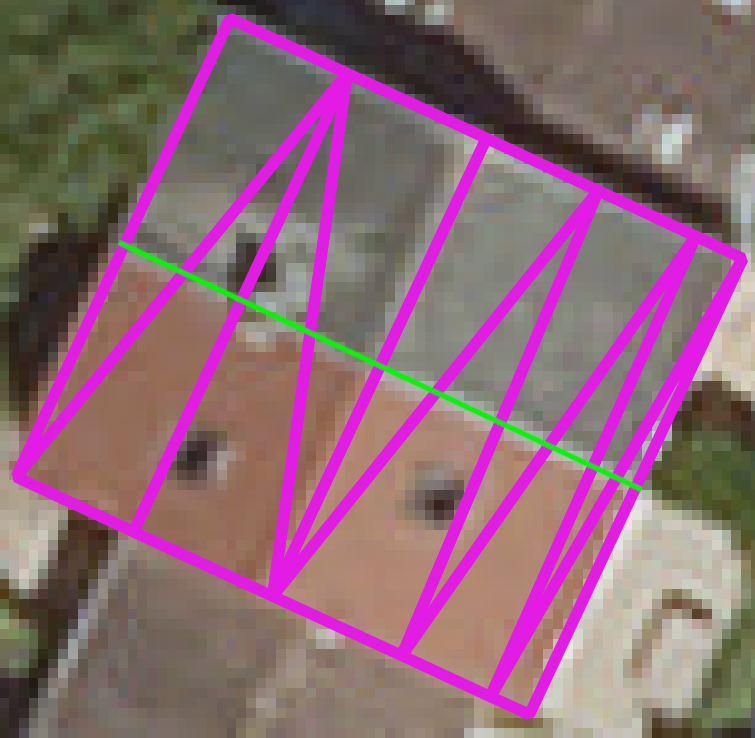
\includegraphics[width=6cm]{images/errors/building/under_segmentation}
                    }{
                        \caption[
                            Nadir projection of an erroneous building superposed on the corresponding orthoimage showing a \texttt{\acrshort*{acr::bus}} error.
                        ]{
                            \label{fig::bus_2d}
                            Nadir projection of an erroneous building superposed on the corresponding orthoimage showing a \texttt{\gls{acr::bus}} error.
                            We can recognize, based on the color differences of roof tiles, the existance of two buildings instead of one.
                        }
                    }
                \end{figure}

                This is a very common error which results from a faulty footprint of the building.
                The latter is either retrieved automatically during the modeling~\parencite{lafarge2012creating}, or is provided as input~\parencite{durupt2006automatic}.
                The first case is the most error inducing one as it relies on extrinsic large-scale remote sensing data that are devoid of semantics.
                The second one is expected to be more close to the reality, but can be unsuitable if the footprints are outdated or too generalized, as discussed in Section~\ref{subsec::state_of_the_art::building_modeling::building_extraction}.

            \paragraph{\texttt{\acrlong*{acr::bos}}.}
                \texttt{\gls{acr::bos}} corresponds to the case where one building is subdivided into two or more.
                This is the opposite of the previous situation.
                Figure~\ref{fig::bos_2d} shows a single building that, when modeled, was subdivided into three parts.\\

                \begin{figure}[htb]
                    \centering
                    \ffigbox[.75\textwidth]{
                        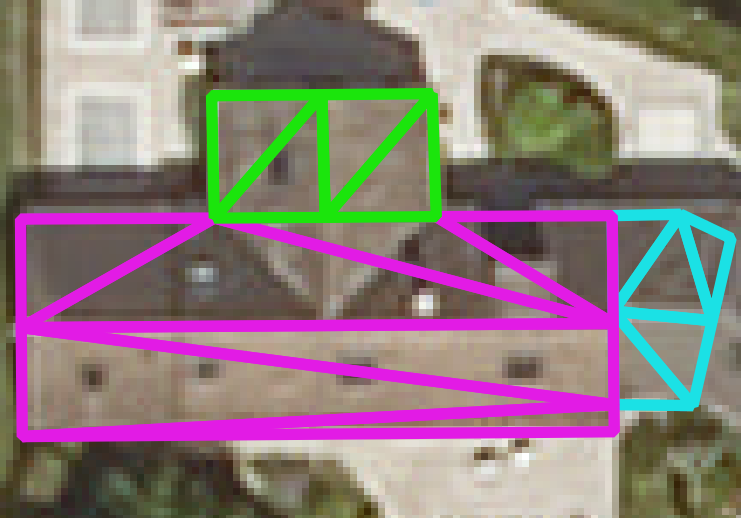
\includegraphics[width=.5\textwidth]{images/errors/building/over_segmentation}
                    }{
                        \caption[
                            Nadir projection of an erroneous building superposed on the corresponding orthoimage showing a \texttt{\acrshort*{acr::bos}} error.
                        ]{
                            \label{fig::bos_2d}
                            Nadir projection of an erroneous building superposed on the corresponding orthoimage showing a \texttt{\acrshort*{acr::bos}} error.
                            We can see how a single building that was modeled into three different ones depicted here in three different colors.
                        }
                    }
                \end{figure}

                This is also a very common error.
                It is the consequence of the same reasons as the under segmentation that was discussed earlier.
                Both these errors are highly semantic and ,thus, creates confusion between both classes.
                Depending on the chosen semantics, a building part (in the sense of CityGML) can be also considered as a single building in other cases.
                These defects depend, actually, on the human perception of buildings and are more ambiguous by nature, unless \textit{explicit} semantic information is provided along the geometry fo the model.
                In fact, there is no combination of geometric characteristic that can help separate buildings, such as convexity or compactness.
                This issue is expected to weight negatively on the predictive capacity of the proposed evaluation approach as will be further studied in Section~\ref{sec::experiments::scalability}.

            \paragraph{\texttt{\acrlong*{acr::bib}}.}
                \texttt{\gls{acr::bib}} corresponds to the case where at least one building footprint border is incorrectly located.
                A sample is shown in Figure~\ref{fig::bib}.\\

                \begin{figure}[htb]
                    \centering
                    \ffigbox[\textwidth]{
                        \begin{subfloatrow}
                            \ffigbox[.48\textwidth]{
                                \includestandalone[mode=buildmissing, width=.45\textwidth]{figures/errors/building/correct_bib}
                            }{
                                \caption{
                                    \label{subfig::gt_bib_3d}
                                    Ground truth \gls{acr::3d} model.
                                }
                            }
                            \qquad
                            \ffigbox[.48\textwidth]{
                                \includestandalone[mode=buildmissing, width=.45\textwidth]{figures/errors/building/bib}
                            }{
                                \caption{
                                    \label{subfig::bib_3d}
                                    \gls{acr::3d} models with an imprecise border (in red).
                                }
                            }
                        \end{subfloatrow}
                    }{
                        \caption{
                            \label{fig::bib}
                            Illustration of a \texttt{\gls{acr::bib}} error.
                        }
                    }
                \end{figure}

                \begin{figure}[htb]
                    \centering
                    \ffigbox[.75\textwidth]{
                        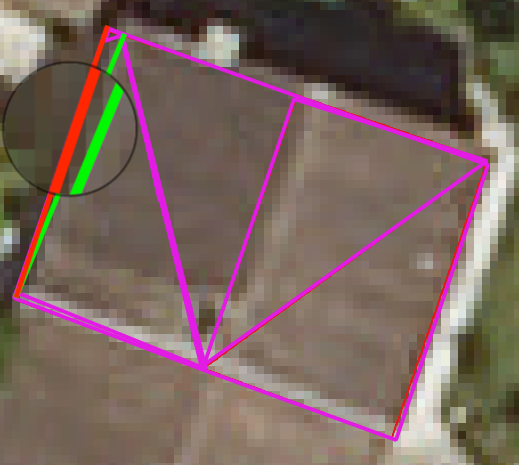
\includegraphics[width=.5\textwidth]{images/errors/building/border}
                    }{
                        \caption[
                            Nadir projection of an erroneous building superposed on the corresponding orthoimage showing a \texttt{\acrshort*{acr::bib}} error.
                        ]{
                            \label{fig::bib_2d}
                            Nadir projection of an erroneous building superposed on the corresponding orthoimage showing a \texttt{\acrshort*{acr::bib}} error.
                            In red is the reconstructed model border that is misestimated, as can be checked in the orthoimage.
                            We can distinguish in green the actual edge using a Nadir projection.
                        }
                    }
                \end{figure}

                This is a purely geometric error that is caused by an imprecise footprint.
                Actually, semantics play a role as \texttt{\gls{acr::bib}} is mainly linked to the end user preferences: one can ignore errors up to a certain threshold. 
                As with previous \texttt{\gls{acr::bus}} and \texttt{\gls{acr::bos}} errors, the footprint border precision is understandably susceptible on the quality of the input data used for modeling.
                It is also expected that the error detection precision will hinge on the resolution of the used reference data and its registration accuracy.
                Regarding automatic modeling methods, border imprecision can be attributed to the quality of the used edge detection algorithms~\parencite{baillard1999automatic,werner2002new,nan2015template} or inaccurate surface estimation\footnote{
                    The border is computed as intersection of the detected surfaces.
                }~\parencite{durupt2006automatic,xiong2014graph}.
                Outside the scope this study, one can try also to estimate the imprecision so as to correct the reconstruction.

            \paragraph{\texttt{\acrlong*{acr::bit}}.}
                \texttt{\gls{acr::bit}} corresponds to the case where the building footprint suffers from topological defects.
                Modeled as a \gls{acr::2d} flat surface, the cases that fall into this label are:
                \begin{description}
                    \item[Missing inner court:] It corresponds to a missing hole (cf. Figure~\ref{subfig::building_hole});
                    \item[Inaccurate border shape:] It is due to a wrong primitive fitting: the shape of the footprint can be better described by a different geometrical shape.
                            Figure~\ref{fig::bit_2d} gives an example where the polygon has a wrong number of sides.
                            Another case is where a circular footprint can be approximated by a polygon.
                \end{description}

                \begin{figure}[htb]
                    \centering
                    \ffigbox[\textwidth]{
                        \begin{subfloatrow}
                            \ffigbox[.48\textwidth]{
                                \includestandalone[mode=buildmissing, width=.45\textwidth]{figures/errors/building/correct_bit}
                            }{
                                \caption{
                                    \label{subfig::gt_bit_3d}
                                    Ground truth \gls{acr::3d} model.
                                }
                            }
                            \qquad
                            \ffigbox[.48\textwidth]{
                                \includestandalone[mode=buildmissing, width=.45\textwidth]{figures/errors/building/bit}
                            }{
                                \caption{
                                    \label{subfig::bit_3d}
                                    \gls{acr::3d} models with an inaccurate topology.
                                    The concerned borders are in yellow.
                                }
                            }
                        \end{subfloatrow}
                    }{
                        \caption{
                            \label{fig::bit}
                            Illustration of a \texttt{\gls{acr::bit}} error.
                        }
                    }
                \end{figure}

                \begin{figure}[htb]
                    \centering
                    \ffigbox[.75\textwidth]{
                        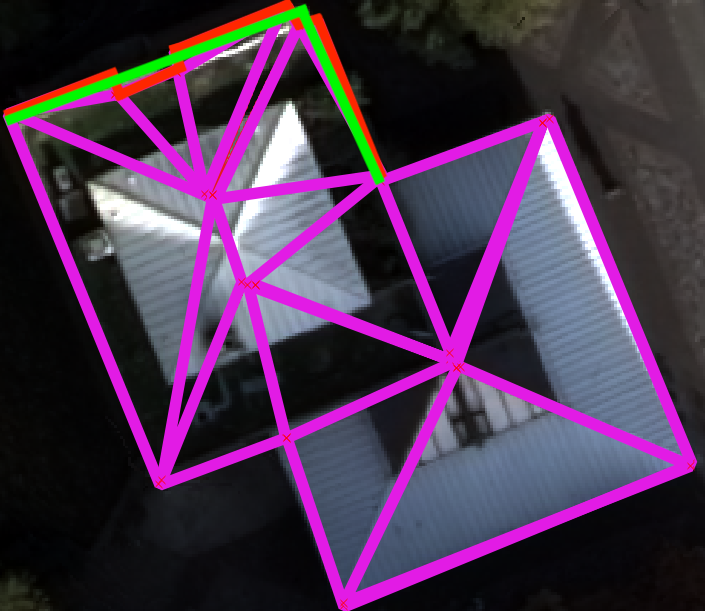
\includegraphics[width=.5\textwidth]{images/errors/building/topology}
                    }{
                        \caption[
                            Nadir projection of an erroneous building superposed on the corresponding orthoimage showing a \texttt{\acrshort*{acr::bit}} error.
                        ]{
                            \label{fig::bit_2d}
                            Nadir projection of an erroneous building superposed on the corresponding orthoimage showing a \texttt{\acrshort*{acr::bit}} error.
                            We can identify (in green) the correct footprint shape compared to the one that was reconstructed (in red).
                        }
                    }
                \end{figure}

                This error, as the earlier one, is a result of a defective edge estimation.
                The main difference between both of them states in the fact that \texttt{\gls{acr::bib}} is geometric in nature while \texttt{\gls{acr::bit}} is topological.
                Both errors are independent and can overlap.

            \paragraph{\texttt{\acrlong*{acr::big}}.}
                \texttt{\gls{acr::big}} corresponds to the case of inaccurate building geometric estimation.

                \begin{figure}[htb]
                    \centering
                    \ffigbox[\textwidth]{
                        \begin{subfloatrow}
                            \ffigbox[.48\textwidth]{
                                \includestandalone[mode=buildmissing, width=.45\textwidth]{figures/errors/building/correct_big}
                            }{
                                \caption{
                                    \label{subfig::gt_big_3d}
                                    Ground truth \gls{acr::3d} model.
                                }
                            }
                            \qquad
                            \ffigbox[.48\textwidth]{
                                \includestandalone[mode=buildmissing, width=.45\textwidth]{figures/errors/building/big}
                            }{
                                \caption{
                                    \label{subfig::big_3d}
                                    \gls{acr::3d} models with an imprecise height estimation.
                                }
                            }
                        \end{subfloatrow}
                    }{
                        \caption{
                            \label{fig::big}
                            Illustration of a \texttt{\gls{acr::big}} error.
                        }
                    }
                \end{figure}

                Up to \gls{acr::lod}-1, it coincides with height imprecision, as depicted in Figure~\ref{fig::big}.
                This is yet again a geometric error.
                Semantics play a role in the definition of the height of a building.
                It can be defined as the height at the highest point, the mediane height or any other valid alternative.
                In case of evaluating at higher than \gls{acr::lod}-2, this error is not reported as it becomes redundant with errors delineated below.
                In fact, if a geometric error is detected at the facet level then it will naturally impact negatively on the geometry of the model as a whole.
            
        \subsubsection{\texttt{Facet Errors} family.}
            In this Section, \gls{acr::lod}-2 and \gls{acr::lod}-3 corresponding \texttt{atomic} errors are presented.

            \paragraph{\texttt{\acrlong*{acr::fus}}.}
                \texttt{\gls{acr::fus}} corresponds to the case where one facet is subdivided into two or more facets.
                This is the same kind of error as \texttt{\gls{acr::bus}} but at the facet level.\\

                \begin{figure}[htb]
                    \centering
                    \ffigbox[\textwidth]{
                        \begin{subfloatrow}
                            \ffigbox[.48\textwidth]{
                                \includestandalone[mode=buildmissing, width=.45\textwidth]{figures/errors/facet/correct_fos_fus_fib_fig}
                            }{
                                \caption{
                                    \label{subfig::gt_fus_3d}
                                    Ground truth \gls{acr::3d} model.
                                }
                            }
                            \qquad
                            \ffigbox[.48\textwidth]{
                                \includestandalone[mode=buildmissing, width=.45\textwidth]{figures/errors/facet/fus}
                            }{
                                \caption{
                                    \label{subfig::fus_3d}
                                    \gls{acr::3d} model with a \texttt{\gls{acr::fus}} error.
                                    The erroneous facet is colored in blue.
                                }
                            }
                        \end{subfloatrow}
                    }{
                        \caption{
                            \label{fig::fus}
                            Illustration of a \texttt{\gls{acr::fus}} error.
                        }
                    }
                \end{figure}

                \begin{figure}[htb]
                    \centering
                    \ffigbox[.75\textwidth]{
                        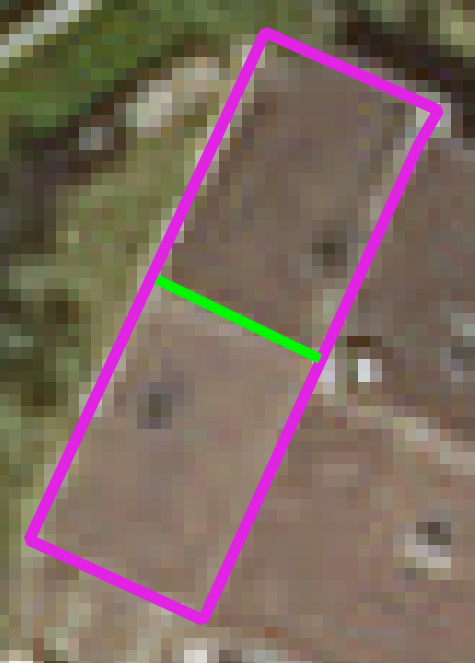
\includegraphics[width=6cm, angle=270]{images/errors/facet/under_segmentation}
                    }{
                        \caption[
                            Nadir projection of an erroneous building superposed on the corresponding orthoimage showing a \texttt{\acrshort*{acr::fus}} error.
                        ]{
                            \label{fig::fus_2d}
                            Nadir projection of an erroneous building superposed on the corresponding orthoimage showing a \texttt{\acrshort*{acr::fus}} error.
                            It shows a case where a higher neighboring building part can drive a misestimation of both facet planes which end up confused in one flat roof.
                            The line segment highlighted in green gives away the fact that the roof was undersegmented.
                        }
                    }
                \end{figure}

                Usually automatic reconstruction methods rely on an initial surface (usually plane) extraction step that generates proposals for further refinement.
                Noise from stereo pairing or missing data in point clouds result in imprecisions in elementary surface retrieval which then lead to surfaces being confused.
                The accuracy drops even further in some cases.
                For instance, superstructures like dormer windows can be big enough to be confused with the roof facets.
                Another setting where surfaces are hard to extract occurs when a building part is shadowed by an other that is higher.
                This is depicted in Figure~\ref{fig::fus_2d}.
                Methods relying only on plane extraction~\parencite{taillandier2004automatic,durupt2006automatic,nan2017polyfit} are particularly vulnerable to this error type.\\

                This defect can be mitigated through the use of \gls{acr::3d} lines as cues to guide the plane extraction~\parencite{zebedin2008fusion,sinha2009piecewise}.
                One can also discard plane extraction alltogether and try to reconstruct the building surface based only on \gls{acr::3d} lines (in other words, a wireframe building model)~\parencite{hofer2017efficient,langlois2019surface}.
                Using grammars of possible stuctures is another alternative, provided it is adequate to the modeled building.
                \textcite{lafarge2008structural} fits the best type of roof models to alleviate issues caused by high levels of noise like when working with Satellite based \glspl{acr::dsm}.
                In some cases, there may be no remedy for the issue, as the used grammar is not exhaustive enough, a \gls{acr::3d} line goes undetected or even a human operator intervention is unable to dispel the ambiguity.

            \paragraph{\texttt{\acrlong*{acr::fos}}.}
                \texttt{\gls{acr::fos}} corresponds to the case where two or more facets are modeled as one, as illustrated in Figure~\ref{fig::fos}.
                This is to \texttt{\gls{acr::bos}} what \texttt{\gls{acr::fus}} is to \texttt{\gls{acr::bus}}.\\

                \begin{figure}[htb]
                    \centering
                    \ffigbox[\textwidth]{
                        \begin{subfloatrow}
                            \ffigbox[.48\textwidth]{
                                \includestandalone[mode=buildmissing, width=.45\textwidth]{figures/errors/facet/correct_fos_fus_fib_fig}
                            }{
                                \caption{
                                    \label{subfig::gt_fos_3d}
                                    Ground truth \gls{acr::3d} model.
                                }
                            }
                            \qquad
                            \ffigbox[.48\textwidth]{
                                \includestandalone[mode=buildmissing, width=.45\textwidth]{figures/errors/facet/fos}
                            }{
                                \caption{
                                    \label{subfig::fos_3d}
                                    \gls{acr::3d} model with a \texttt{\gls{acr::fos}} error.
                                    In green are colored the erroneous edges.
                                }
                            }
                        \end{subfloatrow}
                    }{
                        \caption{
                            \label{fig::fos}
                            Illustration of a \texttt{\gls{acr::fos}} error.
                        }
                    }
                \end{figure}

                \begin{figure}[htb]
                    \centering
                    \ffigbox[.75\textwidth]{
                        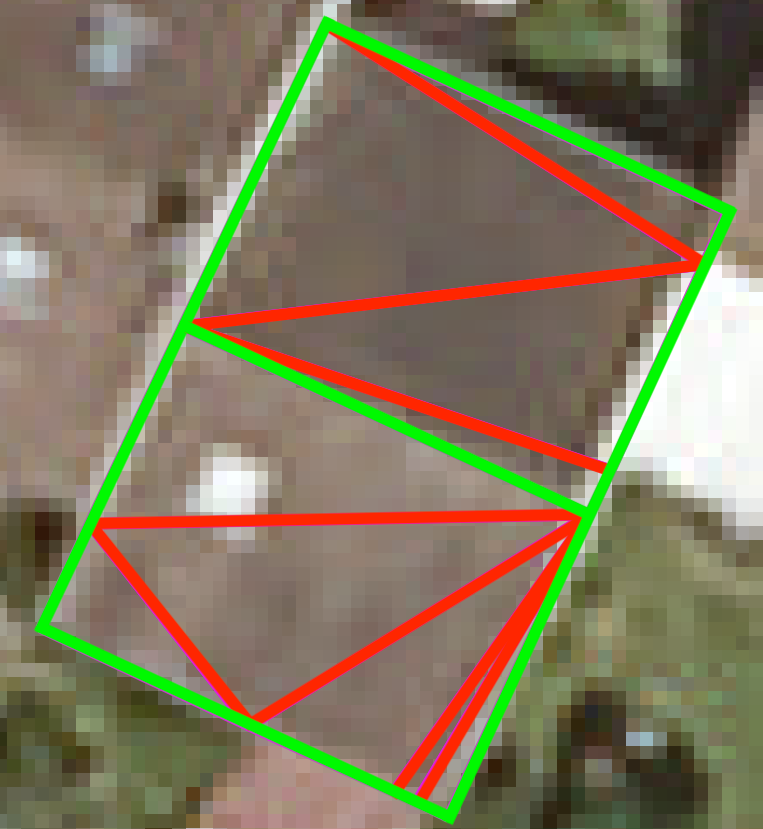
\includegraphics[height=.5\textwidth, angle=270]{images/errors/facet/over_segmentation}
                    }{
                        \caption[
                            Nadir projection of an erroneous building superposed on the corresponding orthoimage showing a \texttt{\acrshort*{acr::fos}} error.
                        ]{
                            \label{fig::fos_2d}
                            Nadir projection of an erroneous building superposed on the corresponding orthoimage showing a \texttt{\acrshort*{acr::fos}} error.
                            A slim chimney in the below corner of the ridge results in a defect ladden \gls{acr::dsm} which translates into an oversegmentation.
                            The erroneous edges are colored in red.
                            One can check using the orthoimage that these are not real.
                        }
                    }
                \end{figure}

                As seen previously, lines are used to help find correct planes and avoid under segmentation.
                However, an overdetection of lines can lead to an oversegmentation of the model.
                This is not rare due to problems that can be encountered with illumination conditions: for instance, a roof structure can cast its shadow on a neighbooring one and cause a gradient in image signal that will be translated to a virtual edge.
                Superstructures play also a negative role just as explained previously.
                This time it is the ones that are small in planar size compared to the noise order of magnitude that are not detected but add bumps that pollute the signal and result in an misestimation of planes.
                High neighbooring buildings are also to blame due to the same reasons as with \texttt{\gls{acr::fus}}, but this time they result in bumps like with superstructures.\\

                To solve this kind of issues, mesh simplification techniques can be helpful.
                In fact,~\textcite{verdie2015lod} uses this approach to smooth away these problems and produce a good generalization of the underlying buildings.
                Another way is to filter the extracted lines relying on redundancy as shown in~\textcite{michelin2013quality}.
                Grammar based methods can equally come to rescue.
                As an example,~\textcite{bredif20073d} uses a set parameteric models in order to model superstructures and better fit \gls{acr::lod}-2 roof facets.

            \paragraph{\texttt{\acrlong*{acr::fib}}.}
                \texttt{\gls{acr::fib}} corresponds to the case where at least one facet border is incorrectly located.
                As an example, Figure~\ref{fig::fib_2d} shows that the central edge that links the two main roof sides does not correspond to the one on the image position.
                This is a purely geometrical error similarly to \texttt{\gls{acr::bib}}.\\

                \begin{figure}[htb]
                    \centering
                    \ffigbox[\textwidth]{
                        \begin{subfloatrow}
                            \ffigbox[.48\textwidth]{
                                \includestandalone[mode=buildmissing, width=.45\textwidth]{figures/errors/facet/correct_fos_fus_fib_fig}
                            }{
                                \caption{
                                    \label{subfig::gt_fib_3d}
                                    Ground truth \gls{acr::3d} model.
                                }
                            }
                            \qquad
                            \ffigbox[.48\textwidth]{
                                \includestandalone[mode=buildmissing, width=.45\textwidth]{figures/errors/facet/fib}
                            }{
                                \caption{
                                    \label{subfig::fib_3d}
                                    \gls{acr::3d} model with a \texttt{\gls{acr::fib}} error.
                                    The misplaced edge is colored in red.
                                }
                            }
                        \end{subfloatrow}
                    }{
                        \caption{
                            \label{fig::fib}
                            Illustration of a \texttt{\gls{acr::fib}} error.
                        }
                    }
                \end{figure}

                \begin{figure}[htb]
                    \centering
                    \ffigbox[.75\textwidth]{
                        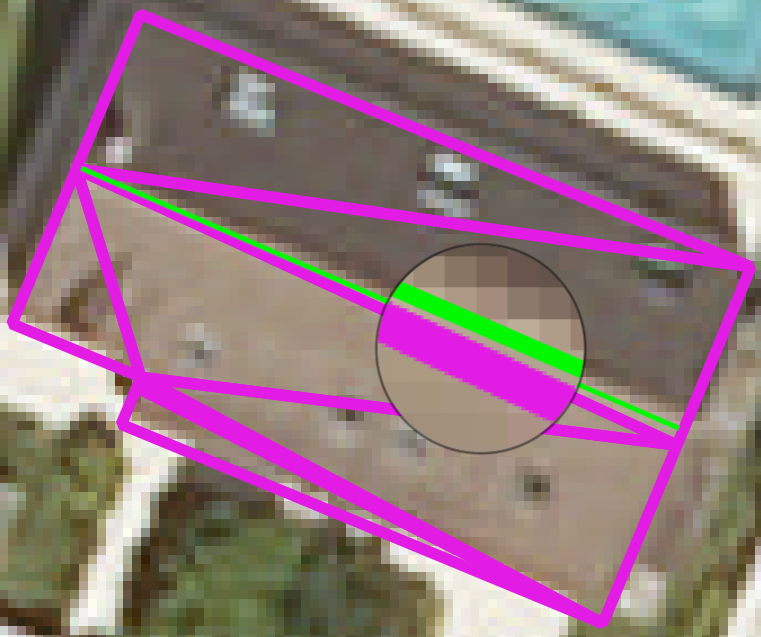
\includegraphics[width=.5\textwidth]{images/errors/facet/border}
                    }{
                        \caption[
                            Nadir projection of an erroneous building superposed on the corresponding orthoimage showing a \texttt{\acrshort*{acr::fib}} error.
                        ]{
                            \label{fig::fib_2d}
                            Nadir projection of an erroneous building superposed on the corresponding orthoimage showing a \texttt{\acrshort*{acr::fib}} error.
                            The real location of the edge is shown in green.
                        }
                    }
                \end{figure}

                Line extraction is usually very faithfull to the data and depends mostly on the resolution and quality of the input data used for modeling.
                The most likely reason usually behind this kind of errors is usually imprecise fitting of primitives that leads to a shifted intersecting edge such as shown in Figure~\ref{fig::fib_2d}.\\

                Just as with oversegmentation, one way to make line retrieval more accurate is to rely on redundancy by extracting them from different modalities.
                An alternative is to rely on symmetries~\parencite{verma20063d} to automatically correct surface intersections.

            \paragraph{\texttt{\acrlong*{acr::fit}}.}
                \texttt{\gls{acr::fit}} corresponds to the case where the facet suffers from topological defects such as wrong primitive fitting (for example, a dome approximated by planar polygons).
                In Figure~\ref{fig::fit}, we can observe how two cylindrical towers were reconstructed as a rectangular parallelepiped.\\

                \begin{figure}[htb]
                    \centering
                    \ffigbox[\textwidth]{
                        \begin{subfloatrow}
                            \ffigbox[.48\textwidth]{
                                \includestandalone[mode=buildmissing, width=.45\textwidth]{figures/errors/facet/correct_fit}
                            }{
                                \caption{
                                    \label{subfig::gt_fit_3d}
                                    Ground truth \gls{acr::3d} model.
                                }
                            }
                            \qquad
                            \ffigbox[.48\textwidth]{
                                \includestandalone[mode=buildmissing, width=.45\textwidth]{figures/errors/facet/fit}
                            }{
                                \caption{
                                    \label{subfig::fit_3d}
                                    \gls{acr::3d} model with a \texttt{\gls{acr::fit}} error.
                                    The facet in yellow has a missing hole.
                                }
                            }
                        \end{subfloatrow}
                    }{
                        \caption{
                            \label{fig::fit}
                            Illustration of a \texttt{\gls{acr::fit}} error.
                        }
                    }
                \end{figure}

                \begin{figure}[htb]
                    \centering
                    \ffigbox[.75\textwidth]{
                        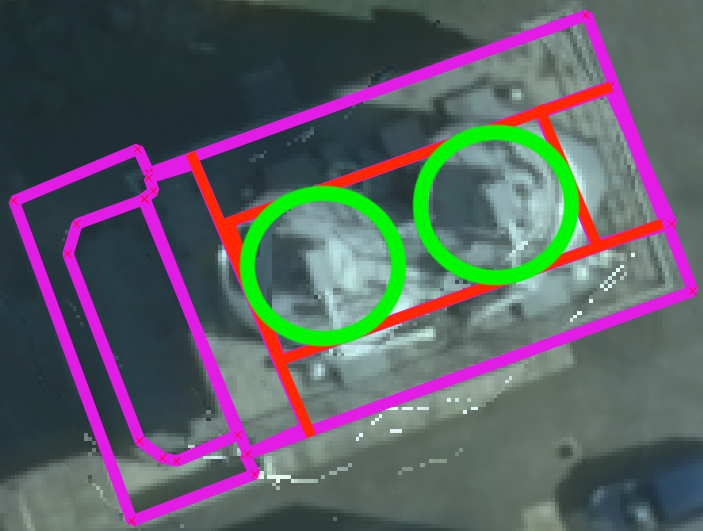
\includegraphics[width=.5\textwidth]{images/errors/facet/topology}
                    }{
                        \caption[
                            Nadir projection of an erroneous building superposed on the corresponding orthoimage showing a \texttt{\acrshort*{acr::fit}} error.
                        ]{
                            \label{fig::fit_2d}
                            Nadir projection of an erroneous building superposed on the corresponding orthoimage showing a \texttt{\acrshort*{acr::fit}} error.
                            The true form (in green) of the towers that is completly misrepresented (in red).
                        }
                    }
                \end{figure}

                This can be due to various reasons.
                Most methods rely on the assumption that buildings are piecewise linear~\parencite{nan2017polyfit} or Manhattan-world like~\parencite{li2016manhattan}.
                This is evidently not always the case (cf. Figure~\ref{fig::fit_2d}).
                Even with the right assumptions, this specific case cannot have been well modeled.
                If so it would have at least approximated the circular cylindrical structures with a regular polygon cylinder.
                This is due to the fact that the quality of the data was poor and was unreliable as explained in the \texttt{\gls{acr::fus}} case in Figure~\ref{fig::fus_2d}.
                The same effect can cause a missing hole being undetected.\\

                Solving this issue is hard besides the obvious change of primitive assumptions.
                It depends highly on the quality of the data.
                One can try to overcome this issue once again, like with the undersegmentation problem, thanks to line detections to reveal convoluted structures when relying on plane extraction only.
                Usually, this problem can be efficiently solved relying mainly on human operators.

            \paragraph{\texttt{\acrlong*{acr::fig}}.}
                \texttt{\gls{acr::fig}} corresponds to the case of inaccurate facet geometric estimation.
                In mathematical terms, this means that the surface primitive parameters are misestimated.
                In Figure~\ref{subfig::fig_3d}, the planar surface slope was miscalculated as flat while it was of \textit{ca.} \SI{25}{\degree}.\\

                \begin{figure}[htb]
                    \centering
                    \ffigbox[\textwidth]{
                        \begin{subfloatrow}
                            \ffigbox[.48\textwidth]{
                                \includestandalone[mode=buildmissing, width=.45\textwidth]{figures/errors/facet/correct_fos_fus_fib_fig}
                            }{
                                \caption{\label{subfig::gt_fig_3d} Ground truth \gls{acr::3d} model.}
                            }
                            \qquad
                            \ffigbox[.48\textwidth]{
                                \includestandalone[mode=buildmissing, width=.45\textwidth]{figures/errors/facet/fig}
                            }{
                                \caption{
                                    \label{subfig::fig_3d}
                                    \gls{acr::3d} model with a \texttt{\gls{acr::fig}} error.
                                    The facet in purple has a wrong slope: It is flat instead of being sloped.
                                }
                            }
                        \end{subfloatrow}
                    }{
                        \caption{
                            \label{fig::fig}
                            Illustration of a \texttt{\gls{acr::fig}} error.
                        }
                    }
                \end{figure}

                \begin{figure}[hbt]
                    \centering
                    \ffigbox[.75\textwidth]{
                        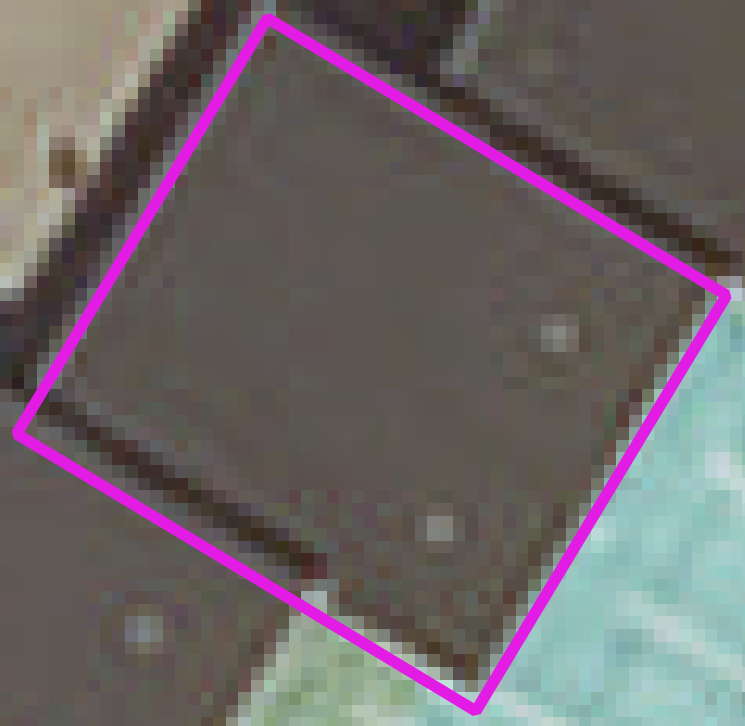
\includegraphics[width=6cm]{images/errors/facet/geometry}
                    }{
                        \caption[
                            Nadir projection of an erroneous building superposed on the corresponding orthoimage showing a \texttt{\acrshort*{acr::fig}} error.
                        ]{
                            \label{subfig::fig_2d}
                            Nadir projection of an erroneous building superposed on the corresponding orthoimage showing a \texttt{\acrshort*{acr::fig}} error.
                            This kind of error is impossible is vizualize on the orthoimage.
                            Projected on the \gls{acr::dsm}, we can reveal the sloped character of the face.
                        }
                    }
                \end{figure}

                This is linked in particular to the input sensor data quality.
                The case of Figure~\ref{subfig::fig_2d} illustrates how neighbooring building parts influence the data as it blunts away the slope of the roof.
                Semantics play again a role in detecting a purely geometric error.
                For correction, as the corruption in the data resulting from the modeling limits could be filtered out using semantics, one can reestimate the parameters of the primitives.
                Failing that, this correction step is usually conducted by human operators.

    \subsection{Discussion}
        \label{subsec::semantic_evaluation::overhead::discussion}

        In the previous subsection, we defined \texttt{atomic} errors based on our observations related to automatic overhead modeling of urban scenes.
        We also discussed how each type of defects can occur and how to proceed in order to correct them.
        Herein, we explore the properties of the ensuing taxonomy of errors.
        In addition, we also discuss the relation between this taxonomy and the ones existing in the litterature.

        \subsubsection{Error taxonomy properties.}
            The similarity of the \texttt{Building Errors} and \texttt{Facet Errors} is striking.
            Indeed, this is what was intended.
            The idea came after observing that segmentation issues can occur both at building and facet errors.
            It was ruled that both should be separated as they occur at different \glspl{acr::lod} so as to have a fine representation of those defects as discussed in Section~\ref{subsec::semantic_evaluation::general_framework::error_classification}.
            If \texttt{atomic} errors are defined on particular defects observed only at a certain level, one can expect that these definitions are going to be too specific and not exhaustive enough.
            This was the case of an earlier categorization of errors based only on a smaller subset of our datasets~\parencite{ennafii2018semanticunannotated}.
            For instance, at building level, in our dataset, missing courts are fairly present.
            However, there are no cases where facets have holes like illustrated in Figure~\ref{subfig::facet_hole}.
            Both can be grouped in one single label ``missing hole''.
            This example, illustrated in Figure~\ref{fig::holes_levels}, makes the case for using similarity across \glspl{acr::lod} being instrumental for generalizability.\\
            This will also be an interesting option to use even if the error families were different as was proposed in Section~\ref{subsec::semantic_evaluation::general_framework::error_classification}.\\

            \begin{figure}[htb]
                \centering
                \ffigbox[\textwidth]{
                    \begin{subfloatrow}[2]
                        \ffigbox[.48\textwidth]{
                            \includestandalone[mode=buildmissing, width=.45\textwidth]{figures/errors/holes/building}
                        }{
                            \caption{
                                \label{subfig::building_hole}
                                A hole at building (viewed from the top) level (\gls{acr::lod}-1) corresponds to an internal court.
                            }
                        }
                        \ffigbox[.48\textwidth]{
                            \includestandalone[mode=buildmissing, width=.45\textwidth]{figures/errors/holes/facet}
                        }{
                            \caption{
                                \label{subfig::facet_hole}
                                Example of a facet (\gls{acr::lod}-2) with a rectangular hole corresponding to a balcony.
                            }
                        }
                    \end{subfloatrow}
                }{
                    \caption{
                        \label{fig::holes_levels}
                        Holes observed at different \glspl{acr::lod}.
                    }
                }
            \end{figure}

            Defining errors in \gls{acr::3d} is not an easy task.
            The \textit{implicit} semantics, discussed in Section~\ref{subsubsec::introduction::urban_3d_reconstruction::building_3d_modeling::semantics}, implies the fact that each facet of the model is special and has a meaning.
            Each facet contained in the model is, hence, supposed to be unique and persistent: it cannot be replaced by an approximating set of different facets as in a mesh.
            This meant that evaluating a whole building model amounts to evaluating each facet individually.
            This simplifies greatly the issue as one can think about the problem moslty as a \gls{acr::2d} evaluation one.
            In fact, the first four \texttt{atomic} errors, at each level, involve only \gls{acr::2d} sufaces, which in the case of planar surfaces amount to polygon evaluation.
            The last error is the only one that takes into account the \gls{acr::3d} ascpect of the facets.
            This explains why border imprecisions (which are geometric issues) were separated from the other geometric inaccuracies.
            These latter errors are, in fact, somewhat overlapping.
            These discussed properties does not only help the generalizability and exhaustivity in the overhead case, but can also be applied to terrestrial based fa\c{c}ade modeling.
            In fact, the same \texttt{atomic} errors can describe perfectly the possible errors that can affect facets on a fa\c{c}ade, owing always to the effect of \textit{implicit} semantics on building models.
        
        \subsubsection{Related taxonomies.}
            This Section discusses the semantic error defnitions in the state-of-the-art.
            As mentioned in Section~\ref{subsec::state_of_the_art::quality::output::semantic},~\textcite{rottensteiner2012isprs} proposed two semantic errors ``over segmentation'' and ``under segmentation''.
            These, however, relate only to facets.
            \textcite{xiong2014graph}, although not aiming at evaluating the quality of a model in its entirety, provides some error labels relative to their reconstruction method.
            For instance, ``Missing Node'' (\textit{resp.} ``False Node'', ``Missing Edge'' and ``False Edge'') correspond to, or are included in, the topological \texttt{atomic} errors from the \texttt{Facet Errors} family: \texttt{\gls{acr::fus}} (\textit{resp.} \texttt{\gls{acr::fos}}, \texttt{\gls{acr::fit}}, and \texttt{\gls{acr::fit}}).\\

            On the other hand, the taxonomy developed by~\textcite{michelin2013quality} is the closest to ours.
            In fact, footprint errors could be reshuffled into \texttt{Building Errors} as \texttt{\gls{acr::bib}} (``erroneous outline'' and ``imprecise footprint'') and \texttt{\gls{acr::bit}} (``missing inner court'').
            Intrinsic reconstruction errors are divided into both levels.
            In fact, ``over-segmentation'', ``under segmentation'' could be part of both \texttt{Building Errors} as well as \texttt{Facet Errors} families.
            ``inaccurate roof'' is a general error that can include \texttt{\gls{acr::fib}} and possibly \texttt{\gls{acr::fit}} also.
            ``Z translation'' is the last label in ``Reconstruction errors'' and is either a \texttt{\gls{acr::big}} error when working at \gls{acr::lod}-0 $\cup$ \gls{acr::lod}-1 level, or included into \texttt{\gls{acr::fig}} if dealing with flat roof facets.
            Finally, ``vegetation occlusion'' and `` non existing'' are gathered into the \texttt{Unqualifiable} label at \texttt{finesse} level 0.\\

            Last,~\textcite{boudet2006supervised} studied rather the acceptability of a model as a whole.
            Confidence in a building model is a subjective assessment of building models that depend on the end user needs.
            Consequently, such a taxonomy cannot directly fit with our labels.
            The acceptability dimension can be incorporated into our framework by attributing a confidence score to each error: for example, a prediction probability.        

\section{Parametric label extraction}
    \label{sec::semantic_evaluation::label_extraction}
    When evaluating building models, not all errors are taken into account depending on the end user needs.
    In fact, labels are extracted according to the taxonomy based on the evaluation settings.
    We will see in this subsection how this is possible and what are the consequences of this choice.

    \subsection{Evaluation parameters}
        At evaluation time, three parameters play a role in determining which error labels to consider.
        We determine hereafter these parameters and their role.\\

        The first parameter is the \textbf{\gls{acr::elod}}.
        Every reconstruction method targets a certain set of \glspl{acr::lod}.
        In consequence, when assessing a reconstruction, a \gls{acr::lod} must be specified.
        At a given \gls{acr::elod}, all error families involving higher orders will be ignored.\\
        Depending on the target of the qualification process, a \texttt{finesse} level might be preferred.
        This corresponds to the second parameter called \textbf{\gls{acr::efin}}.
        It specifies the appropriate semantic level at which errors will be reported.\\
        The last one is error \textbf{exclusivity}.
        It derives from the established family error hierarchy.
        If \textbf{exclusivity} is set \textsc{on} errors of a given \gls{acr::lod}-$l$ family are prioritized over ones with higher \glspl{acr::lod}: i.e., \gls{acr::lod} > \gls{acr::lod}-$l$.
        The latter are simply ignored.
        This would useful in the case where the quality evaluation is used by a correction module, either manually or automatically operated.
        In this case, the latter should prioritize solving low \gls{acr::lod} errors rather than trying to solve more detailed ones.
        This stems from the fact that dealing whith low \gls{acr::lod} errors would probably impact the shape of higher \gls{acr::lod} features.
        As a consequence, detecting and correcting the latter rather than prioritizing the low \gls{acr::lod} ones is going to be virtually wasteful in ressources.

    \subsection{Evaluation labels}
        Depending on the previously defined parameters, the considered labels that will be used for the evaluation would differ.
        We will visit herein all the possible cases based on the defined taxonomy for the overhead reconstruction case (cf. Figure~\ref{fig::taxonomy}).
        For this purpose we must first define the function $\operatorname{children}$ that gives the children of a non-leaf node in the taxonomy tree and outputs the same node if it is a leaf:
        \begin{equation}
            \label{eq::children_taxonomy}
            \begin{aligned}
                \operatorname{children}: V &\rightarrow V\\
                n &\mapsto \begin{cases}
                    \left\{n\right\} & n \in L\\
                    \left\{m \in V : (n, m) \in E \right\} & n \notin L
                \end{cases}
            \end{aligned}.
        \end{equation}
        where:
        \begin{conditions}
            V & is the set of all vertices of the taxonomy tree;\\
            L & is the set of leaf nodes in the tree;\\
            E & is the set of edges (directed) in the tree.
        \end{conditions}
        There are eight cases corresponding to one for the case \textbf{\gls{acr::efin}} = 1, three for the error families level and four for the last case of \texttt{atomic} error level.
        
        \begin{enumerate}[label=\roman*)]
            \item \textbf{\gls{acr::efin}} = 1.
                    The model can either be \texttt{Valid} or \texttt{Erroneous}.
                    As discussed previously, most quality evaluation methods reason at this level.
            \item \textbf{\gls{acr::efin}} = 2 and \textbf{\gls{acr::elod}} = \gls{acr::lod}-1.
                    The model can either be \texttt{Valid} or have a \texttt{Building Error}.
            \item \textbf{\gls{acr::efin}} = 2, \textbf{\gls{acr::elod}} = \gls{acr::lod}-2 and the \textbf{exclusivity} is \textsc{on}.
                    The model can either be \texttt{Valid}, have a \texttt{Building Error} or a \texttt{Facet Error}.
            \item \textbf{\gls{acr::efin}} = 2, \textbf{\gls{acr::elod}} = \gls{acr::lod}-2 and the \textbf{exclusivity} is \textsc{off}.
                    The model can either have a \texttt{Building Error} or not.
                    Independently, it can have also a \texttt{Facet Error} or not.
            \item \textbf{\gls{acr::efin}} = 3, \textbf{\gls{acr::elod}} = \gls{acr::lod}-1 and the \textbf{exclusivity} is \textsc{on}.
                    The model can either be \texttt{Valid} or have a \texttt{Building Error}.
                    If the latter is the case, then it is decided if the building model has a \gls{acr::lod}-1 \texttt{atomic} error or not.
                    All the latter errors are considered independently from each other.
            \item \textbf{\gls{acr::efin}} = 3, \textbf{\gls{acr::elod}} = \gls{acr::lod}-1 and the \textbf{exclusivity} is \textsc{off}.
                    The model can have each \gls{acr::lod}-1 \texttt{atomic} error or not independently from the others.
            \item \textbf{\gls{acr::efin}} = 3, \textbf{\gls{acr::elod}} = \gls{acr::lod}-2 and the \textbf{exclusivity} is \textsc{on}.
                    The model can either be \texttt{Valid}, have a \texttt{Building Error} or a \texttt{Facet Error}.
                    If it is affected with a \texttt{Building Error}, then only its corresponding \texttt{atomic} errors are considered being present or not independently.
                    The same decision is applied if \texttt{Facet Error} was detected, but this time with \gls{acr::lod}-2 \texttt{atomic} errors.
            \item \textbf{\gls{acr::efin}} = 3, \textbf{\gls{acr::elod}} = \gls{acr::lod}-2 and the \textbf{exclusivity} is \textsc{off}.
                    The model can have each \texttt{atomic} error (\gls{acr::lod}-1 and \gls{acr::lod}-2) or not independently from the others.
        \end{enumerate}

        This will influence the evaluation pipeline that will be described later in the next chapter.
        Indeed, the latter will provide more insight about how this takes place.


    \chapter{\textsc{A learning approach for quality evaluation}}
        \label{chap::learned_evaluation}
        \minitoc

\vfill

In the previous chapter (Chapter~\ref{chap::semantic_evaluation}), we developped a hierchical and modular taxonomy of errors for the overhead modeling case.
Based on this taxonomy, and depending on the particular needs, specific error labels are extracted and considered during the quality evaluation.\\

In this chapter, we present the second part of our proposed approach.
It is based on formulating the problem as a supervized classification one.
Issues related to the latter are detailed in Section~\ref{sec::learned_evaluation::classification}.
Next, Section~\ref{sec::learned_evaluation::baseline} presents in details the baseline of features extracted out of building \gls{acr::3d} models.
Third and last, advanced features are discussed in Section~\ref{sec::learned_evaluation::richer_features}.
These are proposed to better model defect predictions.

\clearpage

\section{Quality evaluation as classification}
    \label{sec::learned_evaluation::classification}
    In order to satisfy the \textbf{large-scale} condition imposed at Section~\ref{subsec::introduction::contributions::positioning}, we propose to formulate the problem as a supervized learning one.
    Errors are considered as labels while features are computed so as to describe the observed buildings.
    Actually, as a first approach, the existence of all errors is predicted at the building level, even for \texttt{Facet Errors} labels\footnote{These errors are, in fact, by definition more local.}.
    Determining which facet is affected by an error is a much more challenging problem than the previous one.
    That is why the facet level prediction of errors is not explored in this work.
    The goal is, instead, to test the feasibility of the learning approach.\\

    Errors are predicted based on learned statistical characteristics of the evaluated models.
    The learned approach is usually used to take care of highly semantic tasks, such as ours, that are otherwise hard to process using engineered metrics \addref.\\
    Provided an initial manual annotation effort, the prediction phase is fully automatic, as will be proved by experimental results in Chapter~\ref{chap::experiments}.
    In order for this approach to be scalable at large scales, and hence verify the second constraint in Section~\ref{subsec::introduction::contributions::positioning} which is \textbf{automation}, prediction results should be stable enough independently of the urban scene.
    This is fully studied in Chapter~\ref{chap::more_experiments}.\\

    Two aspects should be discussed to in order to apply this approach to the building \gls{acr::3d} model quality evaluation.
    First, as seen in Section~\ref{sec::semantic_evaluation::label_extraction}, the parametric nature of the taxonomy leads to a varying set of labels.
    For this purpose, we describe in Section~\ref{subsec::learned_evaluation::classification::different_porblems} the different classification problems depending on the evaluation parameters.
    Second, the feature extraction procedure should also be compliant with the \textbf{large-scale} objective set beforehand.
    This aspect and more are detailed in Section~\ref{subsec::learned_evaluation::classification::feature_extraction}.
    Third, the classifier should be able to handle the heterogeneity of the feature vector and must adapt to different input vectors types and sizes.
    The choice of classifiers is, hence, discussed in Section~\ref{subsec::learned_evaluation::classification::classifiers}.

    \subsection{Different classification problems}
        \label{subsec::learned_evaluation::classification::different_porblems}
        The nature of the different classification problems are presented in Table~\ref{tab::classification_problems} depending on the three evaluation parameters defined in Section~\ref{sec::semantic_evaluation::label_extraction}.\\

        \begin{table}[htbp]
            \small
            \begin{tabular}{c c c x{11cm}}
                \toprule
                \textbf{\gls{acr::efin}} & \textbf{\gls{acr::elod}} & \textbf{exclusivity} & \textbf{Classification output}\\
                \midrule
                1 & --- & --- & $binary(\texttt{Valid}, \texttt{Erroneous})$\\
                2 & \gls{acr::lod}-1 & --- & $binary(\texttt{Valid}, \texttt{Building Errors})$\\
                2 & \gls{acr::lod}-2 & \textsc{on} & $multi\_class(\texttt{Valid}, \texttt{Building Errors}, \texttt{Facet Errors})$\\
                2 & \gls{acr::lod}-2 & \textsc{off} & $multi\_label(\texttt{Building Errors}, \texttt{Facet Errors})$\\
                3 & \gls{acr::lod}-1 & \textsc{on} & $multi\_stage(\texttt{Valid}, \texttt{Building Errors})$\\
                3 & \gls{acr::lod}-2 & \textsc{on} & $multi\_stage(\texttt{Valid}, \texttt{Building Errors}, \texttt{Facet Errors})$\\
                3 & \gls{acr::lod}-1 & \textsc{off} & $multi\_label(\operatorname{children}(\texttt{Building Errors}))$\\
                3 & \gls{acr::lod}-2 & \textsc{off} & $multi\_label(\operatorname{children}(\texttt{Building Errors})\cup \operatorname{children}(\texttt{Facet Errors}))$\\
                \bottomrule
            \end{tabular}
            \caption{
                \label{tab::classification_problems}
                All possible classification problem types depending of the evaluation parameters:
                \textbf{\gls{acr::efin}}, \textbf{\gls{acr::elod}} and \textbf{exclusivity}.
            }
        \end{table}

        In Table~\ref{tab::classification_problems}, $multi\_class(l_1, l_2, \dots, l_c)$ (\textit{resp.} $multi\_label(l_1, l_2, \dots, l_c)$) corresponds to the multi-class (\textit{resp.} multi-label) setting.
        We note that:
        \begin{equation*}
            multi\_label(\texttt{Valid}, l_1, l_2, \dots, l_c) \equiv multi\_label(l_1, l_2, \dots, l_c).
        \end{equation*}
        $binary$ refers to the special case of $multi\_class$ where $c = 2$: \textit{i.e}
        \begin{equation*}
            binary(l_1, l_2) \equiv multi\_class(l_1, l_2)
        \end{equation*}
        Two consecutive classification problems can be concatenated in a hierchical multi-stage classification:
        depending on the class that is predicted in the first stage multi-class classifier, a second classification problem predicts the existence of some corresponding labels.
        This denoted by:
        \begin{equation*}
            multi\_stage(l_1, l_2, \dots, l_3) \equiv multi\_label(\operatorname{children}(multi\_class(l_1, l_2, \dots, l_3))).
        \end{equation*}
            
        \textbf{\gls{acr::efin}} = 1 level corresponds to the standard binary classification problem: \texttt{Valid} or \texttt{Erroneous}.
        At \textbf{\gls{acr::efin}} = 2, the \textbf{\gls{acr::elod}} can then take two values in the aerial reconstruction case: \gls{acr::lod}-1 or \gls{acr::lod}-2.
        If set at \gls{acr::lod}-1, it is a binary classification problem: \texttt{Valid} or \texttt{Building Errors}.
        For \gls{acr::lod}-2, if the \textbf{exclusivity} is on, it will be a multi-class problem: \texttt{Valid}, \texttt{Building Errors} or \texttt{Facet Errors}.
        If set off, it becomes a multi-label one with the same labels.
        At \textbf{\gls{acr::efin}} = 3 level, if the \textbf{exclusivity} is on, it is a 2-stage classification problem.
        In the first stage, a multi-class task\footnote{It is binary in the spcial case \gls{acr::elod} = \gls{acr::lod}-1, problem, like in the previous semantic degree.}
        predicts the error family, after which a second multi-label problem decides between the predicted error family children.
        If the \textbf{exclusivity} is off, it turns into one stage multi-label problem that predicts the existence of each atomic error corresponding to the chosen \gls{acr::elod}.
    
    \subsection{Feature extraction}
        \label{subsec::learned_evaluation::classification::feature_extraction}
        The proposed quality evaluation approach, being formulated as a supervized classification problem, requires extracting feature vectors describing characteristics of the evaluated model.
        This is possible through the use of the intrinsic properties of the building model, as well as comparisons with external data.\\
    
        Intrinsic feature extraction consists in make use of the geometric structure of the \gls{acr::3d} model.
        Equally, semantics, as well as building model meta-data, could be utilized for the purpose of intrinsically evaluating a model.
        This case corresponds to the minimal amount of information one can use for building model evaluation.
        In this case, we talk about self-evaluation of building models.
        Since we are considering all possible cases, especially automatically reconstructed building models, only the model geometry is guaranteed to be always available.\\
    
        Extrinsic feature extraction relies on comparing the model to an available external data.
        Obviously, high quality reference models are the best type of data to compare the evaluated model to.
        However, taking into consideration the \textbf{large-scale} objective that was fixed earlier (subsection~\ref{subsec::introduction::contributions::use}), this is not a viable solution.
        We rely then on more basic reference data such as remote sensing acquired data that are the basis of large-scale modeling of urban scenes.\\
        For instance, raw depth information can be used in quality evaluation.
        It can prove helpful in detecting geometric defects that are intrinsically of \gls{acr::3d} nature.
        This was illustrated in Figure~\ref{fig::fig}, as comparing the projected model to the orthoimage did not yield anything out of place, contrarily to the \gls{acr::dsm} comparison.
        Depth data can take multiple forms: unstructured point clouds, originating for instance from \gls{acr::lidar} sensors, or dense depth maps such as \gls{acr::dsm} for the overhead case.\\
        Optical images can also be employed in this framework.
        These provide complementary information such as edges (high frequencies, in general) and textures which are suited for inner defect detection as an example (\textit{cf.} Figure~\ref{subfig::fus_2d}).
        This type of data comes usually in two different shapes: oblique images or orthoimages.
    
    \subsection{Classifier choice}
        \label{subsec::learned_evaluation::classification::classifiers}
        The choice of classifiers shoud take into consideration the highly modular nature of the framework with multimodal features involving many parameters.
        Two classifiers where chosen in this study: \gls{acr::rf} and \gls{acr::svm}.
        Both were discussed at great length in Section~\ref{sec::state_of_the_art::mlpr}.
        Hereafter, we explain how each one is used in this setting.\\

        \subsubsection{\acrlong*{acr::rf}}
            \gls{acr::rf} classifiers is a natural choice in our case.
            As seen in Section~\ref{subsubsec::state_of_the_art::mlpr::classifiers::rf}, this type of classifiers can manage a large number of features with different dynamics and coming from multiple modalities.
            In fact, the computed features could be geometric, image based or height based.
            Each one of these modalities can also be heterogeneous in terms of extracted value types, as will be discussed later in Section~\ref{sec::learned_evaluation::baseline}.
            Relying on their bagging property, a high number of trees is required to cover most of the feature space, while a limited tree depth is needed to avoid overfitting during training.
            While the multi-class case is natively taken into account by the \gls{acr::rf} classifier, the multi-label one requires adopting a one-vs-all approach so as to address each label separately.

        \subsubsection{\acrshort*{acr::svm}}
            \glspl{acr::svm} do not manage well enough heterogeneity in feature vectors.
            Moreover, only binary classification is inherently handled.
            However, it offers other advantages that are not met by \gls{acr::rf}.
            In fact, \glspl{acr::svm} can be useful when labels are not equally distributed in the training set.
            This is actually the case of some errors that are rare in our dataset: specifically the inaccurate topology ones (\textit{cf.} Section~\ref{subsec::experiments::datasets::stats}).
            This type of classifiers naturally encorporates kernels such as the ones presented later in Section~\ref{subsec::learned_evaluation::richer_features::graph}.
            Finally, it is also preferred when dealing with high dimensional feature vectors like those produced by \glspl{acr::scatnet} (\textit{cf.} Section~\ref{subsec::learned_evaluation::richer_features::image}).

\section{Feature baseline}
    \label{sec::learned_evaluation::baseline}
    Since there is no comparable work that studied the learned detection of errors defined in Chapter~\ref{chap::semantic_evaluation}, we propose a baseline for each one of the three modalities: geometric, height based and image based features.
    Attributes are kept simple so as to be used in most situations relying on generally available data.
    We avoid computing and comparing \gls{acr::3d} lines~\parencite{michelin2013quality}, correlation scores~\parencite{boudet2006supervised} or any \gls{acr::sfm} based metric~\parencite{kowdle2011active}.
    In addition of being very costly, these features are methodologically redundant with the \gls{acr::3d} modeling techniques.
    They are, hence, vulnerable to the same defects.
    Conversely, evaluation metrics used in the \gls{acr::3d} building reconstruction literature (\textit{e.g.}, \gls{acr::rmse}) are too weak for such a complex task.
    This will be proven later on in Section~\ref{sec::experiments::baseline_feature_analysis}.

    In Section~\ref{subsec::learned_evaluation::baseline::geometric}, we describe the used baseline for geometric features.
    Next, in Section~\ref{subsec::learned_evaluation::baseline::height}, height based features extraction is explained.
    We end with image based features in Section~\ref{subsec::learned_evaluation::baseline::image}.

    \subsection{Geometric features}
        \label{subsec::learned_evaluation::baseline::geometric}
        Given a building model \(\mathsf{M}\), the facet set is denoted by $\mathsf{F_M}$.
        $\forall (f, g) \in \mathsf{F_M} \times \mathsf{F_M} \; f \sim g$ correspond to facets $f$ and $g$ being adjacent: 
        \textit{i.e.}, they share a common edge. As the roof topology graph in~\parencite{verma20063d}, the input building model $\mathsf{M}$ can be seen as a facet (dual) graph:

        \begin{equation}
        	\label{eq::model_graph}
        	\mathsf{M} \triangleq \left(\mathsf{F_M}, \mathsf{E_M} \triangleq \left\{ \left\{f, g\right\} \subset \mathsf{F_M} : f \sim g \right\} \right).
        \end{equation}

        \begin{figure}[htbp]
            \centering
            \includestandalone[mode=buildnew, width=.75\textwidth]{figures/features/geometric}
            \caption{
                \label{fig::geometric_features}
                Computed geometric attributes represented on the dual graph, for facets $f$ and $g$.
                The green vector groups the node (facet) attributes while the blue one shows the edge features.
            }
        \end{figure}

        The dual graph is illustrated in Figure~\ref{fig::geometric_features}.
        For each facet $f \in \mathsf{F_M}$, we compute its degree (\textit{i.e.}, number of vertices; $f \mapsto d\left(f\right) \triangleq \left\lvert\left\{v : v\text{ is a vertex of }f\right\}\right\rvert$), its area $f \mapsto \mathscr{A}\left(f\right)$ and its circumference $f \mapsto \mathscr{C}\left(f\right)$.
        These are all geometric invariants with respect to $\mathbb{R}^3$ isometries, contrarily to facet centroids $\mathscr{G}\left(f\right)$ and normals $\vec{n}\left(f\right)$.
        This is countersteped by looking, for each graph edge $e=\left\{f, g\right\} \in \mathsf{E_M}$, for the distance between facet centroids $\left\{f, g\right\} \mapsto \left\lVert \mathscr{G}\left(f\right) - \mathscr{G}\left(g\right) \right\rVert$ and the angle formed by their normals $\left\{f, g\right\} \mapsto \arccos\left(\vec{n}\left(f\right) \cdot \vec{n}\left(g\right)\right)$.
        Statistical characteristics are then computed over building model facets using specific functions \(\chi\), like a histogram:        

        \begin{equation}
            \label{eq::histogram_extractor}
        	\chi = \chi^p_{\operatorname{histogram}}: l \mapsto \operatorname{histogram}(l, p),
        \end{equation}
        with $p$ standing for histogram parameters. A simpler option could be:
        \begin{equation}
            \label{eq::max_min_mean_med_extractor}
            \chi = \chi_{\max,\min,\operatorname{mean},\operatorname{med}}: l \mapsto \begin{bmatrix}
                \max(l)\\
                \min(l)\\
                \operatorname{mean}(l)\\
                \operatorname{median}(l)
            \end{bmatrix}.
        \end{equation}

        These features are designed for general topological errors.
        For instance, over-segmentation may result in small facet areas and small angles between their normals.
        Conversely, an undersegmented facet would have a large area.
        Later on, the importance of these features will be discussed in details based on experimental results.
        
        Each building $\mathsf{M}$ can consequently be characterized by a geometric feature vector that accounts for its geometric characteristics:

        \begin{equation}
        	\label{eq::geometric_features}
            v_{\text{geometry}}(\mathsf{M}) = \begin{bmatrix}
            	\chi \left(\left(d\left(f\right)\right)_{f \in \mathsf{F_M}}\right)\\
                \chi \left(\left(\mathscr{A}\left(f\right)\right)_{f \in \mathsf{F_M}}\right)\\
                \chi \left(\left(\mathscr{C}\left(f\right)\right)_{f \in \mathsf{F_M}}\right)\\
                \chi \left(\left( \left\lVert \mathscr{G}\left(f\right) - \mathscr{G}\left(g\right) \right\rVert \right)_{\left\{f, g\right\} \in \mathsf{E_M}}\right)\\
                \chi \left(\left( \arccos\left(\vec{n}\left(f\right) \cdot \vec{n}\left(g\right)\right) \right)_{\left\{f, g\right\} \in \mathsf{E_M}}\right)
            \end{bmatrix}.
        \end{equation}

        Additionally to individual facet statistics, regularity is taken into account by looking into adjacent graph nodes as in~\parencite{zhou20102}.
        Such features express a limited  part of structural information.
        Dealing with this type of information implies graph comparisons which are not a genuinely simple task to achieve.
        Since our objective is to build a baseline, this approach has not yet been considered.

    \subsection{Height based features}
        \label{subsec::learned_evaluation::baseline::height}
        Regarding this modality, raw depth information is provided, for a building model \(\mathsf{M}\), by a \gls{acr::dsm} as a \gls{acr::2d} height grid that is cropped to fit the building footprint: $dsm \in \mathbb{R}^{w_{\mathsf{M}} \times h_{\mathsf{M}}}$\footnote{\label{note::w_h}\(w_{\mathsf{M}}\) (\textit{resp.} \(h_{\mathsf{M}}\)) is the grid width (\textit{resp.} height) and is determined by the size of the building and the resolution of the \gls{acr::dsm}.}.
        This type of reference data must date back to the same time where the building models where produced.
        Otherwise a lot of defects will result simply from change in the scenery.\\
        
        \begin{figure}[htpb]
            \centering
            \includestandalone[width=\textwidth, mode=buildnew]{figures/features/height_based}
            \caption{
                \label{fig::height_based_features}
                Height-based features computed from the \gls{acr::dsm} residuals using histograms.
            }
        \end{figure}

        The \gls{acr::dsm} is compared to the model height~\parencite{bredif20073d,zebedin2008fusion}.
        The latter is inferred from its facets plane equations.
        It is rasterized into an grid structure $alt_{\mathsf{M}} \in \mathbb{R}^{w_{\mathsf{M}} \times h_{\mathsf{M}}}$ using the same spatial resolution as $dsm_{\mathsf{M}}$.
        The difference between the two height grids provides a discrepancy map as shown in Figure~\ref{subfig::residuals}).
        A baseline approach is herein proposed relying on the statistics of pixel values computed using the $\chi$ functions (\textit{cf.} Figure~\ref{fig::height_based_features}).\\

        \begin{equation}
            \label{eq::height_based_features}
            v_{\text{height}}\left(\mathsf{M}\right) = \chi \left( dsm_{\mathsf{M}} - alt_{\mathsf{M}} \right).
        \end{equation}

        The histogram could actually be computed for the building alone without taking into account the terrain arround it.
        However, since reference data is unavailable, cropping out the terrain height values implies that the building model footrpint is flawless, which is not the case.
        As a consequence, the heigth discrepancies around the building model are also computed in order to provide some information on the footprint shape, and hence detect \texttt{BIT} or \texttt{BIB} errors.\\

        Equation~\ref{eq::height_based_features} summarizes how building height-based features are computed.
        Different from a \gls{acr::rmse}~\parencite{lafarge2012creating,poullis2013framework}, the histogram captures the discrepancy distribution, which is particularly helpful in detecting undersegmentation defects or geometric imprecision.
        However, as for the previous geometric attributes, the grid structure information coming from the model is lost.
        Errors cannot be spatialized and linked to a specific facet.

    \subsection{Image based features}
        \label{subsec::learned_evaluation::baseline::image}
        The framework is general enough to encompass both orthorectified images and oblique ones.
        For now, we rely only on more accessible orthorectified images, eventhough they can be riddled with artifacts.
        In an ideal scenario, using oriented images is better for edge verification (as already shown in~\parencite{michelin2013quality}) as orthoimages are a byproduct of earlier ones.
        However, in practice, oblique imagery would give rise to other issues, especially, registration problems.\\

        We aim to benefit from the high frequencies in Very High Spatial Resolution optical images.
        Building edges, like any image edge, correspond to sharp discontinuities in images~\parencite{ortner2007building}.
        The latter are detected using gradient filters on images.
        Gradient based features are advantageous compared to any radiometry based ones.
        This is due to the fact that the latter are much less invariant to changes in the than the first ones.
        Indeed, classic Computer Vision techniques rely on gradient based features:~\textcite{lowe2004distinctive,dalal2005histograms}.
        This is adequate to our case where models and images are part of large heterogeneous datasets.\\
        
        We apply this to our context by comparing building model edges to local image gradients.
        We start by projecting building models in the nadir direction.
        For each facet \(f \in \mathsf{F_M}\), this operation takes into account occlusions and results in:
        \begin{description}
            \item[A \gls{acr::2d} polygon:] If the facet is not vertical (\textit{i.e.} \(\vec{n}(f) \cdot \vec{z} \neq 0\)) and not completly occluded by other facets;
            \item[A segment:] If the facet is vertical (\textit{i.e.} \(\vec{n}(f) \cdot \vec{z} = 0\));
            \item[An empty polygon:] If the facet is completly occluded by other facets.
        \end{description}
        The last two cases are filtered out and the final projection consists in a set of polygons forming a partition of the building footprint denoted:
        \begin{equation}
            \label{eq::facet_projections}
            \mathsf{F_M}^q \triangleq \{q(f): f \in \mathsf{F_M}\}
        \end{equation}
        where:
        \begin{description}
            \item[\(q\)] is the function that yields the projection of a facet if it is a polygon or an empty polygon othewise.
        \end{description}

        This projection is compared with a corresponding orthorectified image \(I_{\mathsf{M}} \in \mathbb{R}^{w_{\mathsf{M}} \times h_{\mathsf{M}} \times 3}\) as shown in Figure~\ref{subfig::model_nadir_projection}.
        For each facet projection, we isolate an edge \(s\) (Figure~\ref{subfig::segment_gradient_collinearity}).
        In an ideal setting, gradients computed at pixels $g \in I_{\mathsf{M}}$ that intersect $s$ need to be collinear with its normal $\vec{n}(s)$.
        In consequence, applying the one of the statistics functions $\chi$ defined in Equations~\ref{eq::max_min_mean_med_extractor} or~\ref{eq::histogram_extractor}, we compute the distribution of the cosine similarity between the local gradient and the normal all along that $s$:
        
        \begin{equation}
            \label{eq::corr_seg}
            \mathsf{D}_{\chi}(s, I_{\mathsf{M}}) \triangleq \chi \left( \left(\frac{\nabla I_{\mathsf{M}}\left(g\right) \cdot \vec{n}(s)}{\left\rVert \nabla I_{\mathsf{M}}\left(g\right)\right\rVert}\right)_{\substack{g \in I_{\mathsf{M}} \\ g \cap s \neq \emptyset}} \right).
        \end{equation}

        \begin{figure}[htpb]
            \begin{center}
                \floatbox{figure}{
                    \begin{subfloatrow}[2]
                        \ffigbox[\FBwidth]{
                            \caption{
                                Model facets (each represented by a specific color) are nadir projected onto the orthoimage.
                            }\label{subfig::model_nadir_projection}
                            }			
                            {
                                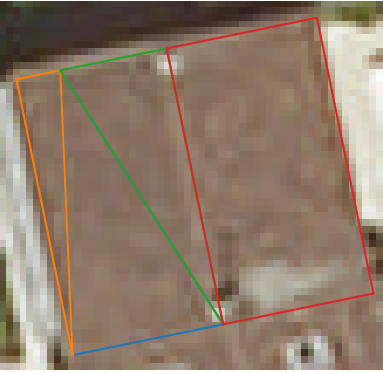
\includegraphics[width=.45\textwidth]{images/features/image/nadir_superposition}
                            }
                        \quad
                        \ffigbox[\FBwidth]{
                                \caption{Local gradients (in purple), on intersecting pixels (in green), are compared to the edge (in red) normal (in black).}
                                \label{subfig::segment_gradient_collinearity}
                            }
                            {\includestandalone[mode=buildnew, width=.45\textwidth]{figures/features/radiometric_features}
                        }
                    \end{subfloatrow}
                }{
                    \caption{Illustration of how features are derived from optical images.}\label{fig::image_based}
                }
            \end{center}
        \end{figure}

        For each polygon \(f^q \in \mathsf{F_M}^q\), the distributions over all its edges\footnote{The empty polygons are ignored as they have no edges.} \(s \in f^q\)\footnote{Abuse of notation.} are stacked to yield a distribution over the whole projected facet.
        In the case of histograms $\chi^p_{\operatorname{histogram}}$ with the same parameters \(p\) (and thus the same bins), it is equivalent to summing out the previous vectors $\mathsf{D}_{\chi^p_{\operatorname{histogram}}}(s, I_{\mathsf{M}})$.
        In order to take into account the variability of segment dimensions, this sum is normalized by segment lengths.\\
        \begin{equation}
            \label{eq::corr_fac}
            D_{\chi^p_{\operatorname{histogram}}}\left(f^q, I_{\mathsf{M}}\right) \triangleq \sum_{s \in q\left(f\right)} \left\rVert s \right\lVert \cdot \mathsf{D}_{\chi^p_{\operatorname{histogram}}}(s, I_{\mathsf{M}}).
        \end{equation}

        The same can be done over all facets of a building $\mathsf{M}$.
        The weights are added in order to take into account the geometry heterogeneity.
        The gradient to normal comparison is similar to the \gls{acr::3d} data fitting term formulated in~\parencite{li2016manhattan}.
        Once again, the model structure is partially lost when simply summing histograms over all segments.

        \begin{equation}
            \label{eq::corr_bul}
            v_{\text{image}}\left(\mathsf{M}\right) = D_{\chi^p_{\operatorname{histogram}}}\left(\mathsf{M}, I_{\mathsf{M}}\right) \triangleq \sum_{f^q \in \mathsf{F_M}^q} \mathscr{A}\left(f^q\right) \cdot \mathsf{D}_{\chi^p_{\operatorname{histogram}}}(f^q, I_{\mathsf{M}}).
        \end{equation}
        
        These image-based attributes are helpful for precision error detection.
        As example, facet imprecise borders can be detected as local gradients direction will be expected to differ greatly from the inaccurate edge.
        It can also be instrumental in under-segmentation detection as colors can change considerably from one facet or one building to another inducing an gradient orthogonal to edge normals.

\section{Advanced features}
    \label{sec::learned_evaluation::richer_features}
    The last section presented features that are by construction taken to be as simple as possible.
    The goal was to test the feasibility of the learned quality evaluation approach.
    This is discussed in length in Section~\ref{sec::experiments::baseline_feature_analysis} and Sections~\ref{sec::more_experiments::finesse} and~\ref{sec::more_experiments::scalability}.\\

    This section presents features that better exploits structural information of the input models that were missed by the baseline.
    In the previous section, we identifed two types of instances from which features are extacted: graph-like and image-like data.
    Advanced graph based feature extractors are proposed in Section~\ref{subsec::learned_evaluation::richer_features::graph}.
    For images-like structures, better attributes are also presented in the next Section~\ref{subsec::learned_evaluation::richer_features::image}.

    \subsection{Graph kernels}
        \label{subsec::learned_evaluation::richer_features::graph}
        In Section~\ref{subsubsec::state_of_the_art::mlpr::feature_extraction::graph_classification}, were discussed some kernels that can describe adequately graphs.
        The geometric baseline features we provided in Section~\ref{subsec::learned_evaluation::baseline::geometric}, more precisely in Equation~\ref{eq::geometric_features}, could actually be seen as a concatenation of the basic feature maps from Equations~\ref{eq::feature_node_graph} and~\ref{eq::feature_edge_graph}.
        This corresponds, in fact, to the basic kernel in Equation~\ref{eq::feature_graph_kernel_sum}.\\

        The biggest disadvantage of this basic kernel is its disregard towards the structural information stored in the graph.
        That is why we propose to use the other kernels that are presented in Section~\ref{subsubsec::state_of_the_art::mlpr::feature_extraction::graph_classification}.
        None of these kernels takes into account edge attributes.
        This is actually not an issue as both the edge attributes of the facet graph (\textit{cf.} Equation~\ref{eq::model_graph}) are in fact a function of node attributes: centroid \(f \mapsto \mathscr{G}\left(f\right)\) and normal \(f \mapsto \vec{n}\left(f\right)\).
        Some of these kernels do not utilize the node attributes either as they take only account of the structure of the graph.\\

        Face normals are unit vectors with coefficients in the interval \([0, 1]\), while centroids are free to be roam in \(\mathbb{R}^3\).
        From a global standpoint, each one of the face geometric features have a specific dynammic.
        As a consequence, taking all these attributes into account by one graph kernel is going to raise some issues.
        One possible solution is to normalize all geometric features, concatenate them and associate the resulting node attribute vectors to one graph.
        We preferred instead to isolate each geometric feature in a specific graph.
        All graphs would share the same structure but each one takes as node attributes a type of geometric features.
        This results in three graphs.
        The first takes the face normals \(f \mapsto \vec{n}\left(f\right)\) as node attributes.
        The second graph has its nodes assigned face centroids \(f \mapsto \mathscr{G}\left(f\right)\).
        The last one has a composite vector
        \begin{equation*}
            f \mapsto \begin{bmatrix}
                d\left(f\right)\\
                \mathscr{A}\left(f\right)\\
                \mathscr{C}\left(f\right)            
            \end{bmatrix}
        \end{equation*} as node attributes.
        The degree, area and circumference, contrarily to the normal and centroid, of facets where inconsequential in error predictions according to the feature importances that were computed when training \glspl{acr::rf}.
        This explains why these were grouped into one vector in contrast with the other two features.\\

        Each graph can take multiple types of kernels.
        We use the kernels described in Section~\ref{subsubsec::state_of_the_art::mlpr::feature_extraction::graph_classification}.
        Since all graphs share the same structure, kernels that ignore node attributes would yield the same results, no matter which node attribute is used.
        There are two such kernels: the random walk kernel and the \gls{acr::svm} \(\vartheta\) kernel.
        We also experimented with three other types of kernels: the Multiscale Laplacian kernel, the propagation kernel and the graph hopper kernel.
        The latter depends on the choice of the base kernel which compares node attributes.
        The \gls{acr::rbf} was briefly experimented and did not yield desirable results.
        Two alternatives were utilized:
        \begin{description}
            \item[Linear kernel:] As shown in Equation~\ref{eq::linear_kernel}, this is the most simple choice;
            \item[Brownian bridge kernel:] This base kernel was originally proposed for the Shortest Path kernel~\parencite{borgwardt2005shortest} and is also valid for its scalable derivation.
        \end{description}
        This results, in total, in \begin{equation*}
            \underbrace{2}_{\substack{\text{kernels ignoring}\\\text{ node attributes}}} + \underbrace{3}_{\substack{\text{attributed}\\\text{graphs}}} \times \left(\underbrace{2}_{\substack{\text{Multiscale Laplacian \&}\\\text{Propagation}}} + \underbrace{1}_{\text{Graph hopper}} \times \underbrace{2}_{\substack{\text{base}\\\text{kernels}}}\right) = 14
        \end{equation*} graph kernels.
        These are aggregated into one kernel using a linear combination.
        This is possible thanks to \gls{acr::mkl} as explained earlier in Section~\ref{subsubsec::state_of_the_art::mlpr::classifiers::svm}.
        Other types of kernels were briefly experimented with, namely the Lov\'asz \(\vartheta\), Graphlet Sampling, Subgraph Matching and Shortest Path kernels.
        However, they did not yield any valuable results and most of the time failed numerically.
        
    \subsection{\acrshort*{acr::scatnet} feature extractor}
        \label{subsec::learned_evaluation::richer_features::image}
        \glspl{acr::cnn} have proven to be the standard feature extractors in image classification.
        However, they require a great load of images in order to learn good enough representations.
        This is not our case as explained later in Section~\ref{subsec::experiments::datasets::stats}.
        As a consequence, we choose instead to use \glspl{acr::scatnet} which mimic classical \glspl{acr::cnn} and can yield good image representations in an unlearned manner as shown in Section~\ref{subsubsec::state_of_the_art::mlpr::feature_extraction::scatnet}.

        \subsubsection{Height based features}
            Discrepancies between the \gls{acr::3d} model extracted height map and the \gls{acr::dsm} manifest in textures in computed residuals (\textit{cf.} Figure~\ref{subfig::residuals}).
            As a matter of fact, \glspl{acr::scatnet} can handle very well texture discrimination as proven theoretically by~\textcite{mallat2012group} and experimentally by~\textcite{bruna2013invariant,sifre2013rotation}.
            In addition, theoretically the height data can be fed directly to a \gls{acr::scatnet} without requiring any normalization or preprocessing since, by construction, they can admit any type of \gls{acr::2d} signal\footnote{There are other versions of \glspl{acr::scatnet} taking one dimensional signals~\parencite{anden2014deep} or even graphs~\parencite{eickenberg2018solid}.}.
            This explains why \glspl{acr::scatnet} were chosen as a height based feature extractor.\\

            From a practical standpoint, the residuals computed as in Section~\ref{subsec::learned_evaluation::baseline::height} come as images in different sizes \(w_{\mathsf{M}} \times h_{\mathsf{M}}\)\cref{note::w_h} depending on the input model.
            Consequently, concatenating \gls{acr::scatnet} coefficients into a single vector is going to result in variable feature vector dimensions.
            One solution is to resize all images to a certain fixed size beforehand.
            However, this solution was quickly ruled out based on few experiments.
            In fact, aside from the fact that this process either looses valuable structural informations or adds undesired blur, it completly deforms the input signal as the \(\frac{w}{h}\) ratio is not guaranteed to constant for all inputs resulting in squashed or elongated image.
            Moreover, since \glspl{acr::scatnet} yields a great deal of coefficients that can easily surpass the number of training instances which hinders the learning ability of any classifier.
            As a consequence, we propose to add a function to help extract meaningful feature vectors with the same length.\\

            Suppose we have a function \(\chi: \mathbb{R}^{w_1 \times d_1} \rightarrow \mathbb{R}^d\) such as the ones presented in Equations~\ref{eq::histogram_extractor} and~\ref{eq::max_min_mean_med_extractor} which has the same output dimension no matter the input size \(w_1 \times d_1\).
            It can be applied on the output of each scattering output \(S_l[dsm - alt](\bullet, p)\):
            \begin{equation}
                \label{eq::reduced_scattering}
                \chi \left(S_m[dsm_{\mathsf{M}} - alt_{\mathsf{M}}]\left(\bullet, p_m\right)\right) \in \mathbb{R}^d.
            \end{equation}
            where:
            \begin{description}
                \item[\(l\)] is the scattering output layer;
                \item[\(p_m\)] is a valid path at layer \(l\) (\textit{cf.} Equation~\ref{eq::scatter_second}). 
            \end{description}
            
            The resulting coefficients defined in Equation~\ref{eq::reduced_scattering} can be concatenated for all \(n_S\) scattering paths to form a feature vector:
            \begin{equation}
                \label{eq::scatnet_height_based_features}
                v_{\text{scattered height}}\left(\mathsf{M}\right) = \begin{bmatrix}
                    \chi \left(S_0[dsm_{\mathsf{M}} - alt_{\mathsf{M}}]\left(\bullet\right)\right)\\
                    \vdots\\
                    \chi \left(S_1[dsm_{\mathsf{M}} - alt_{\mathsf{M}}]\left(\bullet, i_1, \theta_1\right)\right)\\
                    \vdots\\
                    \chi \left(S_2[dsm_{\mathsf{M}} - alt_{\mathsf{M}}]\left(\bullet, i_1, \theta_1, i_2, \theta_2, \xi_2\right)\right)\\
                    \vdots\\
                    \chi \left(S_m[dsm_{\mathsf{M}} - alt_{\mathsf{M}}]\left(\bullet, p_m\right)\right)
                \end{bmatrix}_{
                    \substack{
                        i_1 \in \llbracket 1, I \rrbracket\\
                        \theta_1 \in \frac{\pi}{L} \cdot \llbracket 1, L \rrbracket\\
                        i_2 \in \llbracket i_1 + 1, I \rrbracket\\
                        \theta_2 \in \frac{\pi}{L} \cdot \llbracket 1, L \rrbracket\\
                        \xi_2 \in \llbracket 1, \lfloor\log_2(L)\rfloor \rrbracket\\
                        \vdots\\
                        \lambda_m \in \Lambda_m
                    }
                } \in \mathbb{R}^{d \cdot n_S}.
            \end{equation}
            where:
            \begin{description}
                \item[\(\Lambda_m\)] is the space of all possible values of parameter \(\lambda_m\) at layer \(m\).
            \end{description}

            Regarding the \(\chi\) function it is taken herein as follows:
            \begin{equation}
                \label{eq::max_min_mean_med_std_extractor}
                \chi = \chi_{\max,\min,\operatorname{mean},\operatorname{med},\operatorname{std}}: l \mapsto \begin{bmatrix}
                    \max(l)\\
                    \min(l)\\
                    \operatorname{mean}(l)\\
                    \operatorname{median}(l)\\
                    \operatorname{std}(l)
                \end{bmatrix}.
            \end{equation}
            where:
            \begin{description}
                \item[\(\operatorname{std}(l)\)] computes the standard deviation over the tuple \(l\).
            \end{description}

        \subsubsection{Height based features}
            \glspl{acr::scatnet} seem then to be good choice for image based feature extractors.
            In fact, as shown in Figure~\ref{subfig::bus_2d}, image textures could be also useful for error detection.
            More importantly, as shown with baseline image based features (\textit{cf.} Section~\ref{subsec::learned_evaluation::baseline::image}), edges are key image attributes for comparing building models to orthoimages.
            Actually, \glspl{acr::scatnet} are well suited for edge detection as they use Morlet wavelets for convolution operations (\textit{cf.} Section~\ref{subsubsec::state_of_the_art::mlpr::feature_extraction::scatnet}).
            These filters are adapted to edge detection~\parencite{zhang2007radon}, as depicted in Figure~\ref{subfig::morlet_filters}.\\

            In order to draw features comparing orthoimages to buildings models, we start first by rasterizing the borders of polygons \(f^q \in \mathsf{F_M}\) of the model into a grid structure mask:
            \begin{equation}
                \label{eq::borders_mask}
                Q_{\mathsf{M}} \triangleq \left(\mathbb{1}_{g_{i,j} \cap \left(\bigcup_{f^q \in \mathsf{F_M}}f^q\right)}\right)_{\substack{i \in \llbracket 1, w_\mathsf{M} \rrbracket\\j \in \llbracket 1, w_\mathsf{M} \rrbracket}}
            \end{equation}
            where:
            \begin{description}
                \item[\(g_{i,j}\):] is the rectangle\footnote{It is usually a square as both dimensions are equal.} representing the pixel at row \(i\) and column \(j\).
            \end{description}

            Two options are possible:
            \begin{description}
                \item[\texttt{Deletion}:] Pixels \(g\) in the corresponding orthoimage which are part of a polygon border (\textit{i.e.} \(Q_{\mathsf{M}}(g) = 1\)) are made black:
                        \begin{equation}
                            \label{eq::deletion_orthoimage}
                            I^{\text{dl}}_{\mathsf{M}} \triangleq I_{\mathsf{M}} \odot \left(\begin{bmatrix}
                                1 & 1 & \dots & 1\\
                                1 & 1 & \dots & 1\\
                                \vdots & \vdots & \ddots & 1\\
                                1 & 1 & \dots & 1\\
                            \end{bmatrix} - Q_{\mathsf{M}}^{\otimes 3}\right),
                        \end{equation}
                        where:
                        \begin{description}
                            \item[\(Q_{\mathsf{M}}^{\otimes 3} = Q_{\mathsf{M}} \otimes Q_{\mathsf{M}} \otimes Q_{\mathsf{M}}\)] is the tensor obtained by stacking in depth thee copies of the same matrix \(Q_{\mathsf{M}}\);
                            \item[\(A \odot B  = \left(A_{ij} \cdot B_{ij} \right)_{ij}\)] denotes the Hadamard/Schur product of any two matrices \(A\) and \(B\).
                        \end{description}
                \item[\texttt{Channel}:] The mask \(Q_{\mathsf{M}}\) is simply added to the orthoimage as a fourth channel:
                        \begin{equation}
                            \label{eq::channel_orthoimage}
                            I^{\text{ch}}_{\mathsf{M}} \triangleq I_{\mathsf{M}} \otimes Q_{\mathsf{M}}.
                        \end{equation}
            \end{description}
            The first situation corresponds to an early fusion scheme while the second represent a late fusion case.
            Both settings are experimented with and compared later in Section~\ref{subsec::more_experiments::richer_features::scatnet_baseline}.\\

            Now we can apply the \gls{acr::scatnet} on any of the previously defined images.
            We apply then the same post-processing to yield feature vectors with the same dimensions per channel \(d \cdot n_S\):

            \begin{description}
                \item[\texttt{Deletion}:]
                        \begin{equation}
                            \label{eq::deletion_scanetg_image_based_features}
                            v^{\text{dl}}_{\text{scattered image}}\left(\mathsf{M}\right) \triangleq \begin{bmatrix}
                                \chi \left(S_0[I^{\text{dl}}_{\mathsf{M}}]\left(\bullet\right)\right)\\
                                \vdots\\
                                \chi \left(S_1[I^{\text{dl}}_{\mathsf{M}}]\left(\bullet, i_1, \theta_1\right)\right)\\
                                \vdots\\
                                \chi \left(S_2[I^{\text{dl}}_{\mathsf{M}}]\left(\bullet, i_1, \theta_1, i_2, \theta_2, \xi_2\right)\right)\\
                                \vdots\\
                                \chi \left(S_m[I^{\text{dl}}_{\mathsf{M}}]\left(\bullet, p_m\right)\right)
                            \end{bmatrix}_{
                                \substack{
                                    i_1 \in \llbracket 1, I \rrbracket\\
                                    \theta_1 \in \frac{\pi}{L} \cdot \llbracket 1, L \rrbracket\\
                                    i_2 \in \llbracket i_1 + 1, I \rrbracket\\
                                    \theta_2 \in \frac{\pi}{L} \cdot \llbracket 1, L \rrbracket\\
                                    \xi_2 \in \llbracket 1, \lfloor\log_2(L)\rfloor \rrbracket\\
                                    \vdots\\
                                    \lambda_m \in \Lambda_m
                                }
                            } \in \mathbb{R}^{3 \cdot d \cdot n_S}.
                        \end{equation}
                \item[\texttt{Channel}:]
                        \begin{equation}
                            \label{eq::channel_scatnet_image_based_features}
                            v^{\text{ch}}_{\text{scattered image}}\left(\mathsf{M}\right) \triangleq \begin{bmatrix}
                                \chi \left(S_0[I^{\text{ch}}_{\mathsf{M}}]\left(\bullet\right)\right)\\
                                \vdots\\
                                \chi \left(S_1[I^{\text{ch}}_{\mathsf{M}}]\left(\bullet, i_1, \theta_1\right)\right)\\
                                \vdots\\
                                \chi \left(S_2[I^{\text{ch}}_{\mathsf{M}}]\left(\bullet, i_1, \theta_1, i_2, \theta_2, \xi_2\right)\right)\\
                                \vdots\\
                                \chi \left(S_m[I^{\text{ch}}_{\mathsf{M}}]\left(\bullet, p_m\right)\right)
                            \end{bmatrix}_{
                                \substack{
                                    i_1 \in \llbracket 1, I \rrbracket\\
                                    \theta_1 \in \frac{\pi}{L} \cdot \llbracket 1, L \rrbracket\\
                                    i_2 \in \llbracket i_1 + 1, I \rrbracket\\
                                    \theta_2 \in \frac{\pi}{L} \cdot \llbracket 1, L \rrbracket\\
                                    \xi_2 \in \llbracket 1, \lfloor\log_2(L)\rfloor \rrbracket\\
                                    \vdots\\
                                    \lambda_m \in \Lambda_m
                                }
                            } \in \mathbb{R}^{4 \cdot d \cdot n_S}.
                        \end{equation}
            \end{description}


    \chapter{\textsc{The experimental setup}}
        \label{chap::experimental_setup}
        \minitoc

\vfill

In Chapters~\ref{chap::semantic_evaluation} and~\ref{chap::learned_evaluation}, we proposed a semantic quality evaluation of building \gls{acr::3d} models employing a learning formulation.
Herein, we aim at puting our pipeline to the test using the obtained dataset.
First, in Section~\ref{sec::experiments::datasets}, we delineate how the building models were obtained.
Second and last, Section~\ref{sec::experiments::evaluation} experimentally provides a first outlook of the capacity of our approach to detect errors affecting building \gls{acr::3d} models.

\clearpage

\section{\textsc{Datasets}}
    \label{sec::experiments::datasets}
    
    \subsection{\textsc{Data preprocesing}}
        \label{subsec::experiments::datasets::preprocessing}

    \subsection{\textsc{Urban scenes and modeling techniques}}
        \label{subsec::experiments::datasets::scenes}
        \gls{acr::3d} models from three different cities of France are selected in order to assess the performance of our framework: \textbf{Elancourt}, \textbf{Nantes}, and the XIII\textsuperscript{th} district of Paris (\textbf{Paris-13}) (\textit{cf.} Figure~\ref{fig::france_map}).
        Figure~\ref{fig::elancourt_ortho} depicts the small city of \textbf{Elancourt} which contains diverse of building types: residential areas with gable and hip roof buildings and large industrial flat roof building based districts (\textit{cf.} Subfigure~\ref{subfig::elancourt_samples}).
        \textbf{Nantes}, as shown in Figure~\ref{fig::nantes_ortho}, represents a denser urban setting but with a lower building diversity (\textit{cf.} Subfigure~\ref{subfig::nantes_samples}).
        In Figure~\ref{fig::paris-13_ortho}, one can see how \textbf{Paris-13} consists of mostly flat roof high towers which coexist with Haussmann style buildings that typically exhibit highly fragmented roofs (\textit{cf.} Subfigure~\ref{subfig::paris-13_samples}).
        The \textbf{Elancourt} (\textit{resp.} \textbf{Nantes} and \textbf{Paris-13}) scene contains 2,009 (\textit{resp.} 748 and 478) annotated building models.
        The \gls{acr::dsm} as well as the orthorectified image resolution is \SI{0.06}{\m} for the first area while it is \SI{0.1}{\m} for the other ones.

        \begin{figure}[htpb]
            \ffigbox[\textwidth]{
                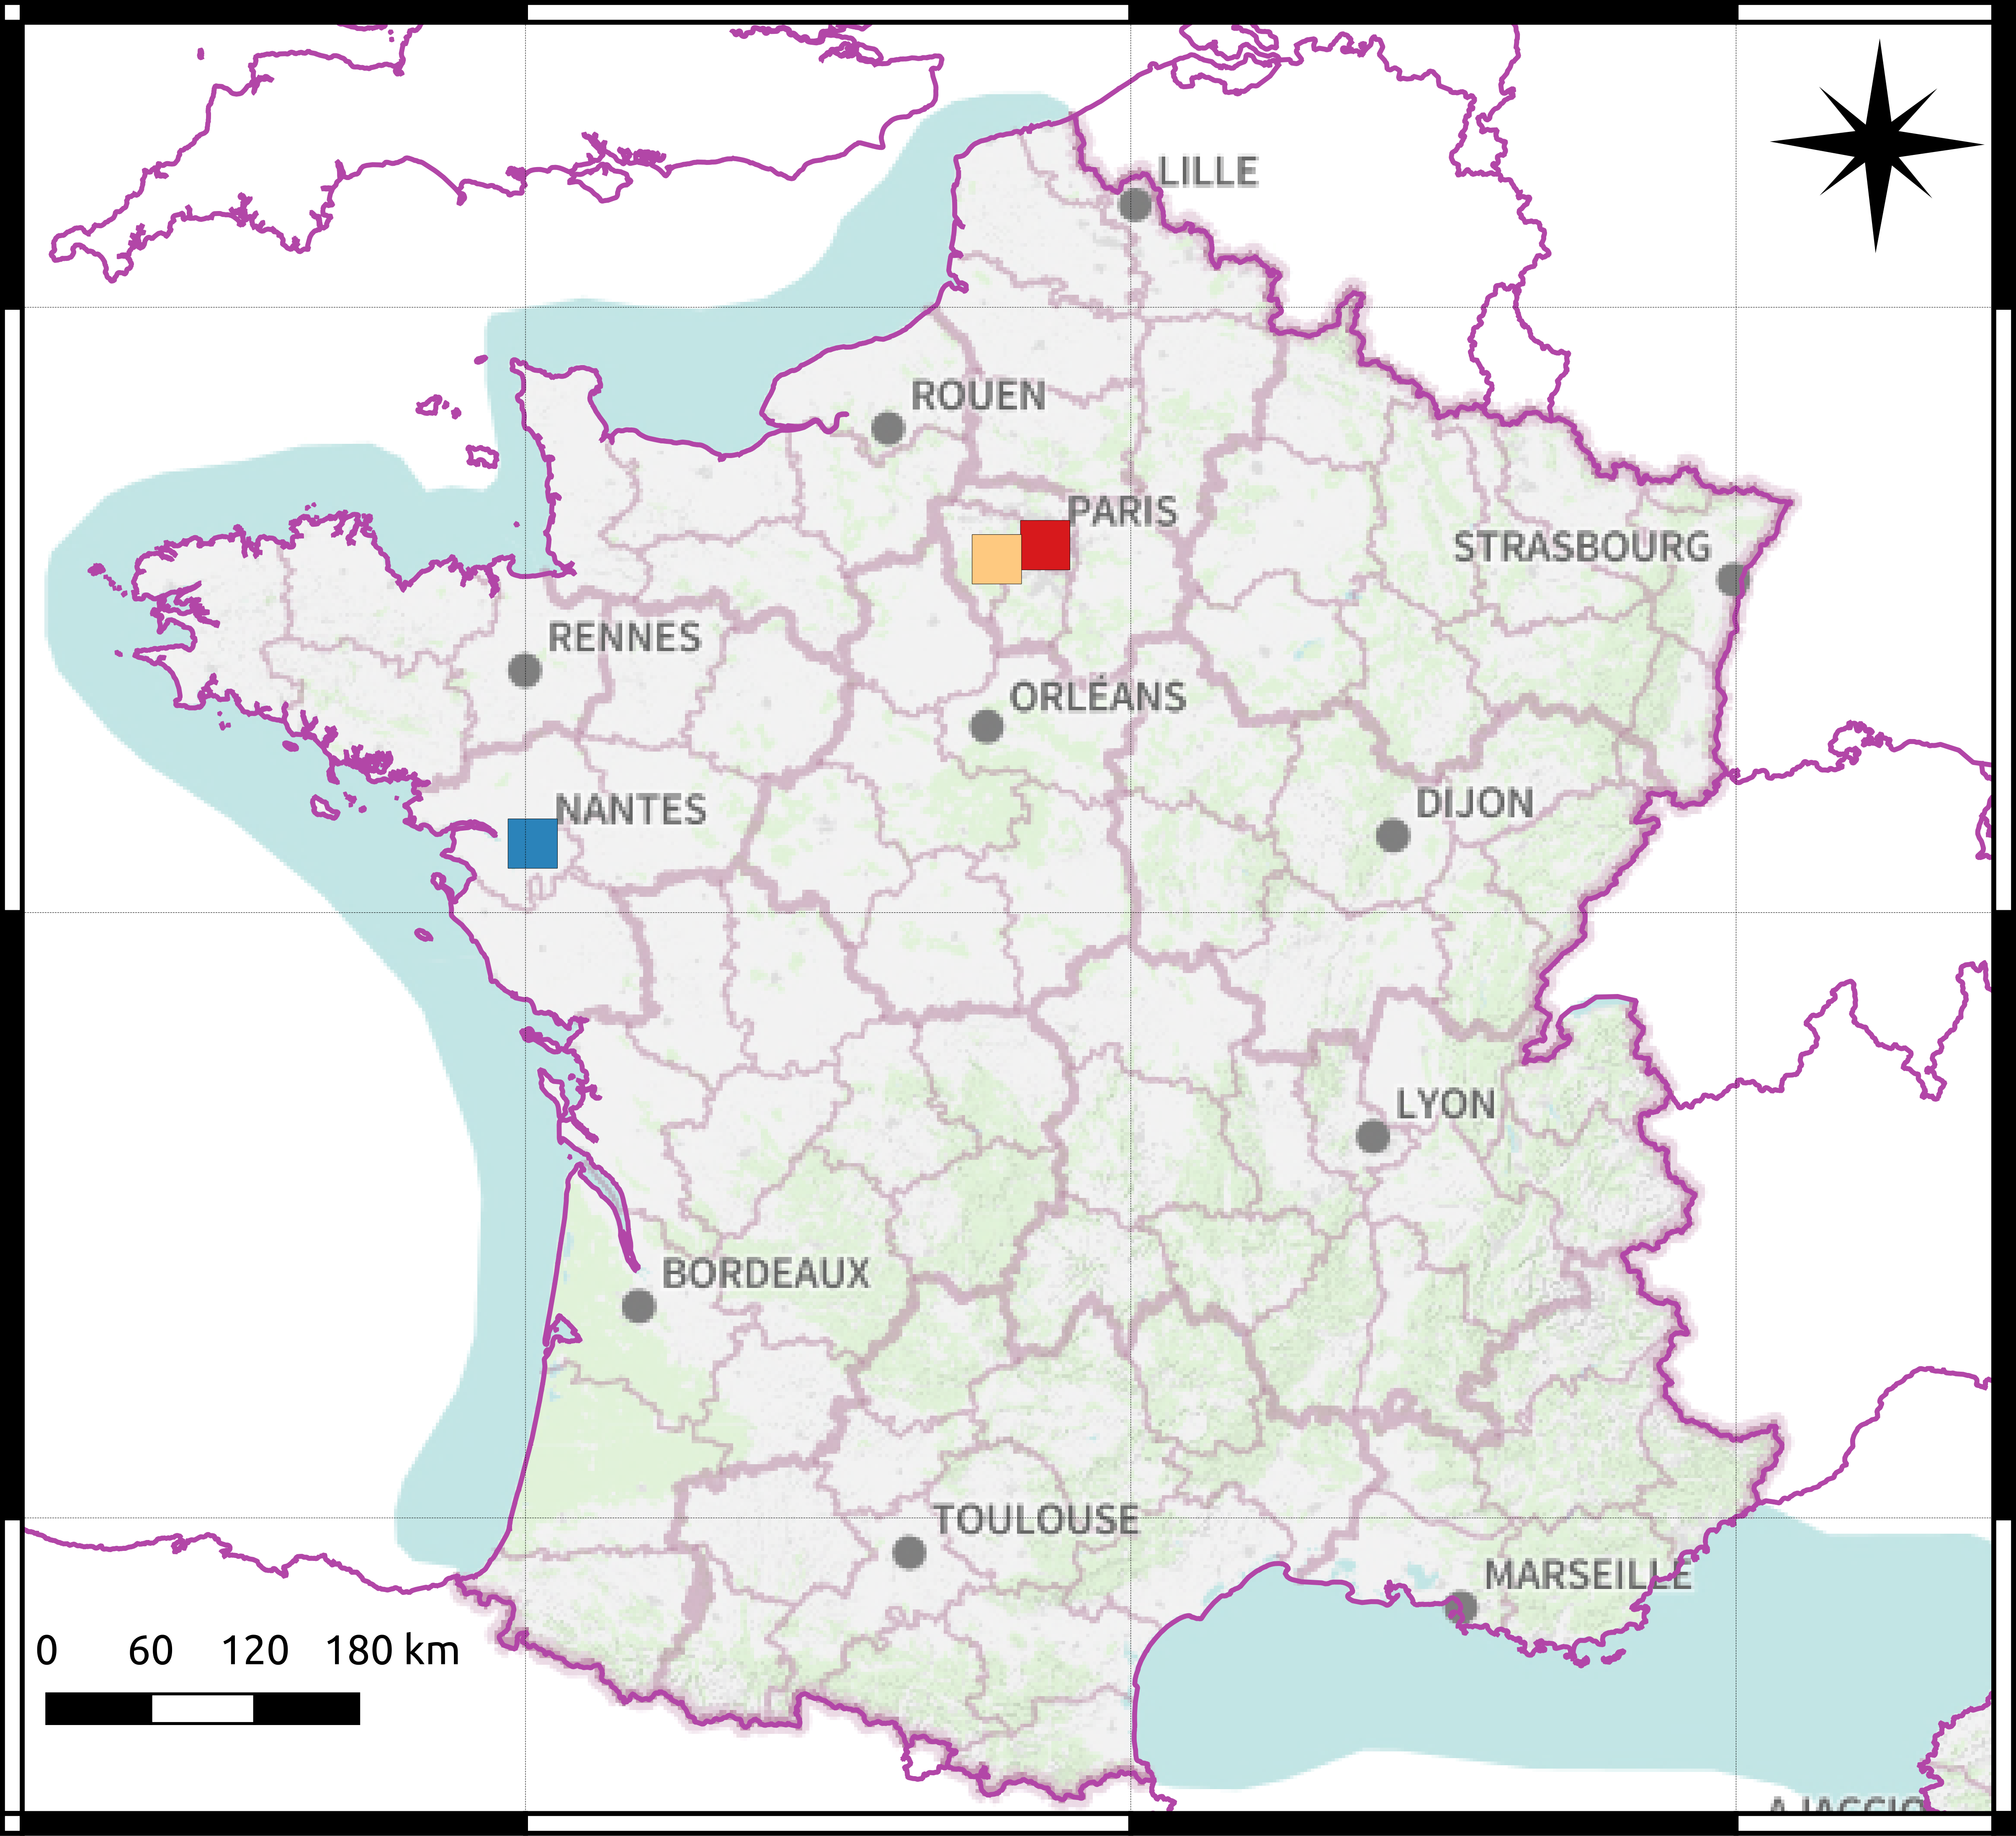
\includegraphics[width=.75\textwidth]{images/datasets/france_map}
            }{
                \label{fig::france_map}
                \caption{
                    Map of France showing the studied urban scenes.
                    Each square corresponds to a city:
                    \textcolor[rgb]{.84,.1,.11}{\(\blacksquare\)} \textbf{Paris-13}, \textcolor[rgb]{1,.79,.5}{\(\blacksquare\)} \textbf{Elancourt}, \textcolor[rgb]{.17,.51,.73}{\(\blacksquare\)} \textbf{Nantes}.
                }
            }
        \end{figure}

        \begin{figure}[htpb]
            \ffigbox[\FBwidth]{
                \includegraphics[width=\textwidth]{images/datasets/elancourt_global}
            }{
                \label{fig::elancourt_ortho}
                \caption{
                    Orthoimage showing the diversity of buildings in Elancourt.
                }
            }
        \end{figure}

        \begin{figure}[htpb]
            \ffigbox[\FBwidth]{
                \includegraphics[width=\textwidth]{images/datasets/nantes_global}
            }{
                \label{fig::nantes_ortho}
                \caption{
                    Orthoimage depicting the dense city center of Nantes.
                }
            }
        \end{figure}

        \begin{figure}[htpb]
            \ffigbox[\FBwidth]{
                \includegraphics[width=\textwidth]{images/datasets/paris-13_global}
            }{
                \label{fig::paris-13_ortho}
                \caption{
                    Orthoimage showing the heterogeneous of the XIII\textsuperscript{th} district of Paris.
                }
            }
        \end{figure}

        \begin{figure}[htpb]
            \ffigbox[\textwidth]{
                \begin{subfloatrow}[3]
                    \ffigbox[\FBwidth]{
                        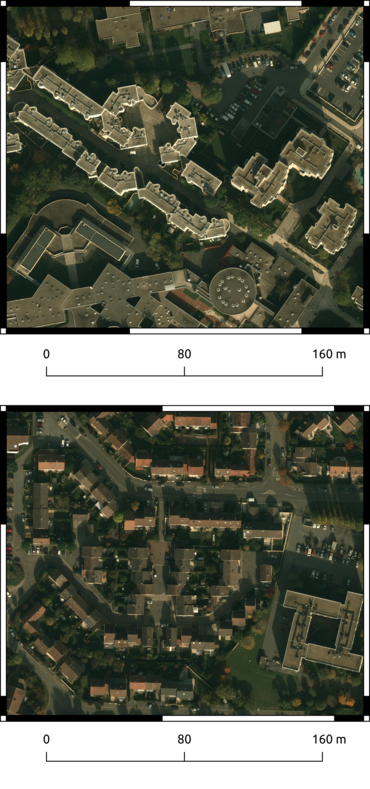
\includegraphics[width=.3\textwidth]{images/datasets/elancourt_samples}
                    }{
                        \label{subfig::elancourt_samples}
                        \caption{
                            Elancourt contains flat roof buildings (top) as well as gable roof ones (bottom).
                        }
                    }
                    \ffigbox[\FBwidth]{
                        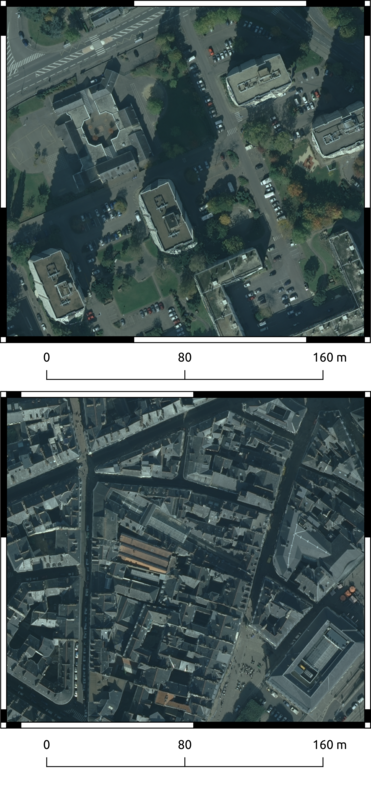
\includegraphics[width=.3\textwidth]{images/datasets/nantes_samples}
                    }{
                        \label{subfig::nantes_samples}
                        \caption{
                            Nantes exhibits high rising towers (top) along side densely packed fragmented roof buildings (bottom).
                        }
                    }
                    \ffigbox[\FBwidth]{
                        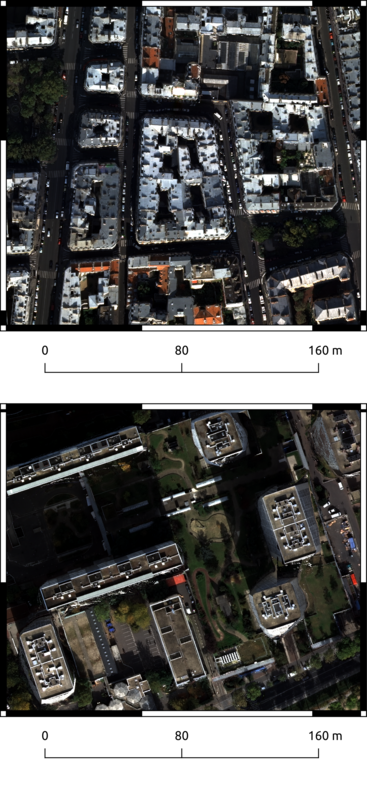
\includegraphics[width=.3\textwidth]{images/datasets/paris-13_samples}
                    }{
                        \label{subfig::paris-13_samples}
                        \caption{
                            The XIII\textsuperscript{th} district of Paris is made of Haussmannian buildings (top) and high rising towers bottom).
                        }
                    }
                \end{subfloatrow}
            }{
                \label{fig::france_map}
                \caption{
                    Samples of building types per region.
                }
            }
        \end{figure}

        \gls{acr::3d} models were generated using the algorithm described in~\parencite{durupt2006automatic}, out of existing building footprints and aerial VHR multi-view \glspl{acr::dsm}.
        The modeling algorithm simulates possible roof structures with facets satisfying some geometric constraints.
        The best configuration is selected using a scoring system on the extrapolated roofs.
        Finally, vertical building fa\c{c}ades connect the optimal roof to the building footprint.
        These models have a \gls{acr::lod}-2 level.
        This method is adapted to roof types of low complexity and favors symmetrical models that are common in residential areas.
        It has been selected to ensure a varying error rate for the three areas of interest, especially since models were generated with partly erroneous cadastral maps.
        3,235 buildings in total are considered.
        They were annotated according to the atomic errors list provided by our taxonomy.

    \subsection{\textsc{Error statistics}}
        \label{subsec::experiments::datasets::stats}

        Some of the models obtained using the previous datasets were annotated manually in order to build training datasets.
        To annotate a building model, the manual operator compares the nadir projection of the model to the corresponding orthoimage and \gls{acr::dsm}.
        This was possible thanks to the work\footnote{\href{https://github.com/CHUPClem/sGrISner.git}{GIS Graphical interface for annotation.}} of Clémence Chupin, who was a Master student at \gls{acr::ensg}.
        Figure~\ref{fig::error_statistics} reports modeling errors statistics over the annotated buildings.

        \begin{figure}[htpb]
            \centering
            \ffigbox[\textwidth]{
                \includestandalone[mode=buildnew, width=\textwidth]{figures/datasets/families_stats}
            }{
                \caption{
                    \label{fig::family_errors}
                    Occurence statistics for error families computed for each area: \texttt{finesse} = 2.
                }
            }
        \end{figure}
        \begin{figure}[htpb]
            \centering
            \ffigbox[\textwidth]{
                \begin{subfloatrow}
                    \centering
                    \ffigbox[\textwidth]{
                        \includestandalone[mode=buildnew, width=\textwidth]{figures/datasets/lod1_stats}
                    }{
                        \caption{
                            \label{subfig::lod1_errors}
                            Occurence statistics for Building errors depending each area.
                        }
                    }
                \end{subfloatrow}
                \vskip1em
                \begin{subfloatrow}
                    \centering
                    \ffigbox[\textwidth]{
                        \includestandalone[mode=buildnew, width=\textwidth]{figures/datasets/lod2_stats}
                    }{
                        \caption{
                            \label{subfig::lod2_errors}
                            Occurence statistics for Facet errors depending each area.
                        }
                    }
                \end{subfloatrow}
            }{
                \label{fig::error_statistics}
                \caption{
                    Error statistics depending on the \texttt{finesse} level.
                    The height of bars indicates the frequency of each errors while the number of occurences is displayed over.
                }
            }
        \end{figure}

        These statistics are first analysed depending on the family errors at the \texttt{finesse} = 2 level (\textit{cf.} Figure~\ref{fig::family_errors}).
        Due to the fact that geometrically inconsistent \gls{acr::3d} models were filtered out in a preprocessing (nadir projection) step, \texttt{Unqualifiable} buildings represent a small fraction of the dataset (less than \SI{7.5}{\percent}).
        Actually, this latter corresponds to the, partially or completly, occluded buildings that could not be qualified.
        Moreover, only a small fraction of buildings are \texttt{Valid}:
        57 (\SI{2.84}{\percent}) in \textbf{Elancourt}, 55 (\SI{7.35}{\percent}) for \textbf{Nantes} and 21 (\SI{4.39}{\percent}) in \textbf{Paris-13}.
        Most buildings are affected by the \texttt{Building Errors} family (over \SI{58.16}{\percent}) and the \texttt{Facet Errors} one (over \SI{75.94}{\percent}).\\

        At the \texttt{finesse} level 3, two axes of analysis are possible.
        First, we group errors that are very frequent in the dataset.
        Over-segmentation errors (\texttt{FOS} and \texttt{BOS}), in both error families, are well represented ranging from \SIrange{38.9}{66.8}{\percent}.
        The same is true for \texttt{FIG} with a frequency from \SIrange{59.8}{80}{\percent}.
        \texttt{FIT}, on the other hand, are very rare in all the areas with ratios a little less than \SI{1.5}{\percent}.
        The rest have a presence ratio within the percentage interval of [10, 30].
        The errors that are rare are understandably going to impact negatively the learning process.\\
        
        Second, we can compare error frequency discrepancies depending on the studied scene.
        \textbf{Elancourt} is different compared to the relatively close sets \textbf{Nantes} and \textbf{Paris-13}, with regards to \texttt{BOS}, \texttt{BUS} and \texttt{BIT}.
        In fact, the last two areas are more densely urbanized than the first one exhibitting the same properties at \gls{acr::lod}-0.
        \texttt{BIB}, on the other hand, are equally distributed over the different datasets as it depends mostly on the input sensor data resolution independently of building types.\\
        At the facet level, \texttt{FIT} is also equally occuring across all the scenes different from the rest of \texttt{Facet errors}.
        In fact, \texttt{FOS} occurence ratio is related to the size of facets in urban scenes.
        Actually, the less complex roof structures are, the more big are facets and the more chance they have to be over segmented.
        Indeed, \textbf{Elancourt}, \textbf{Nantes} and \textbf{Paris-13} scenes are ordered in an ascending manner of their roof structure complexity.
        Conversely, in line with the previous analysis, \texttt{FUS} are less present in \textbf{Elancourt} than in \textbf{Nantes} which, in turn, contains less of the same error than \textbf{Paris-13}.
        \texttt{FIB} is distributed in the same manner as \texttt{FUS}.
        This is mainly due to the fact that the more a roof structure is complex the more precision errors are possible.
        \texttt{FIG} does not keep the same dynamic as its frequency keeps stable from \textbf{Elancourt} and \textbf{Nantes} but jumps considerably in \textbf{Paris-13}.
        This may be explained by the fact that the gap in \texttt{FUS} error ratios between \textbf{Paris-13} and \textbf{Nantes} is more important than that of \texttt{FOS} errors, contrarily to the same gaps for the same errors between \textbf{Nantes} and \textbf{Elancourt} which compensate each other.

\section{\textsc{Pipeline evaluation}}
    \label{sec::experiments::evaluation}
    In the last section, we also explained how we acquired our dataset, in addition to analysing the effect of the urban scene on error statistics.
    Beforehand, all the ingredients needed in the proposed methodology were presented.
    This section aims at specifying how each bloc of the pipeline is implemented.\\

    In Subsection~\ref{subsec::experiments::evaluation::setup} provides all details about our experimental approach.
    Next in Subsection~\ref{subsec::experiments::evaluation::baseline_feature_analysis}, we report some first results using the baseline features we developped.

    \subsection{\textsc{Experimental set-up}}
        \label{subsec::experiments::evaluation::setup}
        In this subsection, we give detailed account of how every building block of our pipeline is parameterized.
        We first start by discussing feature configurations, before defining the taxonomy parameters of interest and endin with a thorough description of the classification process.

        \subsubsection{\textsc{Feature configurations}}
            \label{subsubsec::experiments::evaluation::setup::feature_configurations}
            We present herein the features that were used in experiments.
            First, as we tried to prove the efficiency of the proposed learning framework, we made use different configurations using the baseline features.
            Second, as richer features were used, new combinations were possible and are discussed hereafter.

            \paragraph{Baseline features}
                The geometric features are always available.
                As a consequence, we tested four feature configurations: ``geometric features'' (\textbf{Geom.}) only, ``geometric and height features''(\textbf{Geom.} $\cup$ \textbf{Hei.}), ``geometric and image features''(\textbf{Geom.} $\cup$ \textbf{Im.}) as well as ``geometric, height and image features''(\textbf{All.}).
                In order to have a better compare the important of each modality, the feature vectors they produce are of the same size.
                Actually, using the function \(\chi_{\max,\min,\operatorname{mean},\operatorname{med}}\) defined in Equation~\ref{eq::max_min_mean_med_extractor}, the geometric feature vector in Equation~\ref{eq::geometric_features} is of dimension
                \begin{equation*}
                    \underbrace{4}_{\substack{\text{the output dimension}\\\text{of the function } \chi_{\max,\min,\operatorname{mean},\operatorname{med}} }} \times \underbrace{5}_{\substack{\text{the number of the facet}\\\text{graph attributes}}} = 20.
                \end{equation*}

                Regarding height based feature vectors their dimension depend on the histogram parameters.
                Since we compute differences between observed and model height at terrain level also (\textit{cf.} Subsection~\ref{subsec::learned_evaluation::baseline::height}), and because these are virtually unbounded and can differ from one scene to another, the maximum possible discrepancy is limited to \SI{\pm 50}{\m} for all scenes.
                In order to have the same feature vector dimension for this modality, the number of bins is fixed manually to \(20\).
                For image based features, the cosine similarity between normal vectors, used in Equation~\ref{eq::corr_fac}, is by definition bounded in the interval [-1, 1].
                This interval is consequently divided evenly into \(20\) bins for the histogram computation.
                The \glspl{acr::dsm} and orthorectified images used to derive height and image features have the same spatial resolution as the reconstruction input data.\\

                \sisetup{
                    scientific-notation = true
                }
                These features implementation is conducted in Python and is not thoroughly.
                Geometric features are computed in average in \SI{0.05}{\s \per \building}, height based ones take in average \SI{1.4}{\s \per \building} and finally image based ones need more than \SI{16}{\s \per \building}.
                In order to reduce the runtime of each experiment, the last two types of features are cached once computed for a building model and retrieved latter for tests.

            \paragraph{Richer features}
                Baseline features are replaced by more enhanced ones as shown in Section~\ref{sec::learned_evaluation::richer_features}.
                We lay out herein how their parameters are determined.

                \subparagraph{Graph kernels}
                    In Subsection~\ref{subsec::learned_evaluation::richer_features::graph}, we have seen how 14 graph kernels are aggregated to describe graphs.
                    We relied, in experiments, on an available Python module called GraKel~\parencite{siglidis2018grakel}.
                    We provide herein the parameters of each kernel type.
                    \begin{description}
                        \item[\(\blacktriangleright\) Random walk] The exponential version fails numerically and was left out.
                                    After a grid search \(\lambda\) was set to be \num{1e-3}, for the geometric random walk.
                                    This is actually a very low value as \(\lambda\) has to verify the condition stated in Equation~\ref{eq::condition_geometric_kernel_convergence} for all pairs of graphs in the training dataset.
                                    One case where the largest eigenvalue of the direct product of the adjacency matrix of two graphs in the dataset suffices to considerably lower the maximal value \(\lambda\) can take.
                                    To compute such a kernel it takes approximatly \SI{1.14}{\s\per\building\squared}.
                        \item[\(\blacktriangleright\) \gls{acr::svm} \(\vartheta\)] This kernel takes no parameters.
                                    It takes on average \SI{0.0000201}{\s\per\building\squared} to compute a kernel comparison.
                        \item[\(\blacktriangleright\) Multiscale Laplacian] Our building models have a varying number of nodes from 4 up to 20 facets in some cases.
                                    That is why we choose to keep the same radius size\footnote{The neighboorhoods \(N_l(v)\) are taken as balls around vertex \(v\)~\parencite{kondor2016multiscale}.} and depth level \(L\) set to 3 as in the original paper~\parencite{kondor2016multiscale}.
                                    The same goes for the regularization terms fixed at a value of \num{1e-2}.
                                    Computing one kernel comparison requires around \SI{10.6}{\s\per\building\squared}.
                        \item[\(\blacktriangleright\) Propagation] The choice of the transition matrix, as explained in Sub-subsection~\ref{subsubsec::state_of_the_art::mlpr::feature_extraction::graph_classification}, is set by default to be the normalized adjacency matrix.
                                    The maximal iteration number \(t_{\max}\) is similar to the height parameter of the Weisfeler-Lehman kernel and is set to 5.
                                    Other parameters regarding the hashing and binning processed are kept at their default values.
                                    Comparing two instances takes around \SI{0.0812}{\s\per\building\squared}.
                        \item[\(\blacktriangleright\) Graph hopper] This kernel takes no other parameter than the choice of base kernels.
                                    Comparisons between takes on average \SI{34.5}{\s\per\building\squared}.
                    \end{description}

                \subparagraph{\gls*{acr::scatnet}}
                    For \glspl{acr::scatnet}, we rely on a modern and vestatile Python module: Kymatio~\parencite{andreux2018kymatio}.
                    The parameterization of the \gls{acr::scatnet} does not depend on the signal content as much as it relates to the size of input images.
                    This is true because the filter banks, which parameterization is the most related to the signal dynamics, were set beforehand.
                    As a consequence, the same parameters were applied for image and height based features.\\

                    The number of possible orientations \(L\) is fixed at its default value 8 as it was the optimal choice corresponding to the already defined Morlet filter banks.
                    \(I\) the scale of the \gls{acr::scatnet} pooling operator was set to 3.
                    This corresponds to models \(\mathsf{M}\) verifying: \(w_{\mathsf{M}} \geq 2^3 = 8\) and \(h_{\mathsf{M}} \geq 8\).
                    In \textbf{Elancourt}, it implies that building models have to be at least larger in length and width than \SI{8 x 0.06}{\m} = \SI{0.48}{\m}, while in \textbf{Paris-13} and \textbf{Nantes} the minimal dimensions of a building are \SI{8 x 0.10}{\m} = \SI{0.80}{\m}.
                    This is reasonable and fails only for some rare cases were the building is obviously over segmented an can be detected as such by simply applying a building model size threshold.\\
                    The maximal number of layers \(m\) is 2.
                    As a consequence, the total number, according to Equation~\ref{eq::scatnet_number_paths} of scattering outputs is \(n_S = 217\).
                    This implies that the length of \gls{acr::scatnet} based features is \(d \times n_S\) = \num{5 x 217} = 1085.\\

                    The Kymatio implementation of \gls{acr::scatnet} uses GPU to accelerate computations.
                    Using an NVIDIA GeForce GTX 750 Ti graphics card, it takes around \SI{14.06}{\s \per \building} on average to compute a height based features and \SI{20.86}{\s \per \building}.
                    As with previous features onces they are calculated they are cached for latter use.
                    \sisetup{
                        scientific-notation = false
                    }
    
        \subsubsection{\textsc{Considered labels}}
            All \textbf{\gls{acr::efin}} levels were tested.
            The input models are generalized to \gls{acr::lod}-2.
            As a consequence, we chose \textbf{\gls{acr::elod}} = \gls{acr::lod}-2.
            If the \textbf{exclusivity} is \textsc{on}, at \textbf{\gls{acr::efin}} level 3, the second stage classification results depends on the first one.
            We are, at this stage, trying to prove the feasability, in the first place, of the proposed approach.
            As proven in the latter experiments (\textit{cf.} Section~\ref{sec::more_experiments::finesse}), the first stage results are not good enough in order to test this configuration.
            That is why we limited the experiments to the case where the \textbf{exclusivity} is set to be \textsc{off}.

        \subsubsection{\textsc{Classification settings}}
            Herein, are given extensive details how the considered classifiers (\textit{cf.} Subsection~\ref{subsec::learned_evaluation::classification::classifiers}) are applied.
            We also provide the metrics that will help measure the accuracy of predictions.

            \paragraph{Classifiers}
                As discussed in Subsection~\ref{subsec::learned_evaluation::classification::classifiers}, two classifier types were considered in the experimental study.
                As already explained beforehand in Subsection~\ref{subsec::learned_evaluation::classification::classifiers}, a one-vs-all approach is used to adapt \glspl{acr::rf} to multi-label settings.
                The same approach was choosen to accommodate \glspl{acr::svm} to both the multi-class and the multi-label possibilities.
                We relied upon the already available and ubequitous implementation in Python~\parencite{scikit-learn}.
                Below we detail quantitavely the used parameters.
                
                \sisetup{
                    scientific-notation = true
                }
                \subparagraph{\acrshort*{acr::rf}}
                    A brief grid search involving a smaller set of building models and only baseline geometric features~\parencite{ennafii2018qualificationunannotated} yielded comparable results for the number of trees set in the range \numrange{850}{1000} and a maximum tree depth from \numrange{3}{5}.
                    Given the already immense parameter search space involving all possible feature configurations, feature extraction parameters and label possibilities, the \gls{acr::rf} parameters are set to \num{1000} for the tree number and 4 for the maximum tree depth for all other experiments without performing any grid search.
                    Regarding \gls{acr::scatnet} based features, in Subsection~\ref{subsec::more_experiments::richer_features::scatnet_baseline} were reduced using \gls{acr::pca} and Kernel\footnote{The used kernel is that same the one used with the \gls{acr::svm} classifier.} \gls{acr::pca} in order to not overwhelm the geometric features.
                    To that end, these rich features are reduced to 20 in length to equal the dimension of baseline geometric feature vectors.

                \subparagraph{\acrshort*{acr::svm}}
                    The linear \gls{acr::svm} is not well suited for the type of features that we use, even for baseline features as experiments do not yield any resuslts in time.
                    As a consequence, the latter was left out and we experimented only with the kernel \gls{acr::svm} using the standard \gls{acr::rbf} kernel (\textit{cf.} Equation~\ref{eq::rbf_kernel}) when instances are vectors not graphs.
                    Just as with the \gls{acr::rf} classifier, we conducted a grid search using baseline geometric features only in order to determine both parameters \(C\) and \(\gamma\) by limiting the range between \numrange[range-phrase={ and }]{1e1}{1e-3} for both.
                    All values yielded sensibly the same scores.
                    As a result we set these parameters as follows: \(C = \num{1e-1}\) to not overpenalize nor underfit during learning and \(\gamma = \num{1e-3}\) to avoid overfitting.
                    Regarding \gls{acr::mkl}, we made use of the already implemented EasyMKL~\parencite{aiolli2015easymkl} approach.
                    It was the only method, to our knowledge that was readily available library to use with Python\footnote{\href{https://github.com/IvanoLauriola/MKLpy}{MKLpy}}.
                    \sisetup{
                        scientific-notation = false
                    }
    
            \paragraph{Used metrics}
                The overall accuracy is not interesting due to the highly unbalanced label distribution.
                We prefer reporting recall \(\bm{Rec}\) and precision \(\bm{Prec}\) ratios.
                As a reminder these metrics are defined as follows:
                \begin{align}
                    \label{eq::recall_precision}
                    \bm{Rec} &\triangleq \frac{tp}{tp + fp}\\
                    \bm{Prec} &\triangleq \frac{tp}{tp + fn},
                \end{align}
                where:
                \begin{conditions}
                    tp & the number of instances predicted positive that are positive in reality;\\
                    fp & the number of instances predicted positive that are negative in reality;\\
                    fn & the number of instances predicted negative that are positive in reality.
                \end{conditions}
                Recall expresses, from a number of samples of a given class, the proportion that was rightfully detected as such.
                Precision indicates how much samples, amongst the detected ones, were, in truth, part of the studied class~\parencite{powers2011evaluation}.
                We also summarize these two ratios with their harmonic mean, the F-score:
                \begin{equation}
                    \label{eq::f_score}
                    \bm{F_{score}} \triangleq \frac{2}{\frac{1}{\bm{Rec}} + \frac{1}{\bm{Prec}}}.
                \end{equation}
                Unless said otherwise, all experiments were conducted performing a 10-fold cross validation to avoid overfitting or underfitting issues.
                Only test results are reported.

    \subsection{\textsc{Baseline feature analysis}}
        \label{subsec::experiments::evaluation::baseline_feature_analysis}
        At this stage, we study only the baseline features proposed in Section~\ref{sec::learned_evaluation::baseline}.
        The goal is to assess the added value of each modality.
        First, the \gls{acr::rmse} is proven to be inadequate for detecting errors in our taxonomy.
        Second, prediction results from all possible feature configurations are compared in Subsubsection~\ref{subsubsec::experiments::evaluation::setup::feature_configurations}.
        Third and last, we conclude the analysis by studying the feature importance, for all training zones.

        \subsubsection{\textsc{\acrshort*{acr::rmse} predictive capacity}}
            \label{subsubsec::experiments::evaluation::baseline_feature_analysis::rmse}
            The \gls{acr::rmse} is the standard measure in most of \gls{acr::3d} reconstruction methods.
            As a consequence, we use it herein as a reference that our baseline is to be compared to.
            We train the classifier on Elancourt with the one dimensional feature vector containing the \gls{acr::rmse}.
            This scene was sufficient enough for our analysis.
            Mean test results are shown in Table~\ref{tab::rmse_results}.\\

            \begin{table}[htpb]
                \begin{tabular}{c c c c c c c c c c}
                    \toprule
                    & \texttt{BOS} & \texttt{BUS} & \texttt{BIB} & \texttt{BIT} & \texttt{FOS} & \texttt{FUS} & \texttt{FIB} & \texttt{FIT} & \texttt{FIG} \\
                    \midrule
                    \(\bm{Rec}\) & 99.55 & 0.21 & 0 & 0 & 98.68 & 0.63 & 0 & 0 & 98.15 \\
                    \midrule
                    \(\bm{Prec}\) & 68.78 & 33.33 & --- & 0 & 66.60 & 0.25 & --- & 0 & 61.15 \\
                    \midrule
                    \(\bm{F_{score}}\) & 81.35 & 0.42 & 0 & 0 & 79.52 & 1.24 & 0 & 0 & 75.36 \\
                    \midrule
                    \(\bm{Acc}\) & 68.46 & 75.65 & 89.57 & 94.66 & 66.36 & 83.62 & 88.24 & 98.36 & 60.86 \\
                    \bottomrule
                \end{tabular}
                \caption{
                    \label{tab::rmse_results} \texttt{Finesse} 3 experiment results using \gls{acr::rmse} on Elancourt.
                    \(\bm{Acc}\) expresses the overall accuracy ratio.
                }
            \end{table}

            We can distinguish two groups of errors: 
            \begin{description}
                \item[\texttt{BOS}, \texttt{FOS} and \texttt{FIG}:] These have a high recall and a low precision and overall accuracy;
                \item[\texttt{BUS}, \texttt{BIB}, \texttt{BIT}, \texttt{FUS}, \texttt{FIB} and \texttt{FIT}:] These have low recall and precision ratios.
            \end{description}
            The first (\textit{resp.} second) group coincides exactly with errors that affect more (\textit{resp.} less) than half of the buildings.
            For this kind of errors, the classifier assigns to almost all samples the positive class.
            In fact, we end up with a high ratio of false positives (false alarms) and hence a high recall ratio that is coupled with a weak precision and overall accuracy.
            Exactly the inverse happens with the rest of the errors as we obtain a high percentage of false negative.
            We can safely conclude that the \gls{acr::rmse} is not able to detect errors defined in our taxonomy.

        \subsubsection{\textsc{Feature ablation study}}
            \label{subsubsec::experiments::evaluation::baseline_feature_analysis::ablation}
            We tested the different feature configurations, at \texttt{finesse} level 3 and in all urban zones.
            Mean precision and recall test results are reported in Table~\ref{tab::ablation_f3}.
            F-scores are averaged across all feature configurations and represented in Figure~\ref{fig::f_score_ablation_f3}.\\

            \begin{table}[htpb]
                \small
                \begin{center}
                    \begin{tabular}{| c | c c | c c | c c | c c |}
                        \hline
                        \multicolumn{9}{|c|}{\textbf{Elancourt}}\\
                        \hline
                        &\multicolumn{2}{c|}{\textbf{Geom.}} & \multicolumn{2}{c|}{\textbf{Geom. $\cup$ Hei.}} & \multicolumn{2}{c|}{\textbf{Geom. $\cup$ Im.}} & \multicolumn{2}{x{2.4cm}|}{\textbf{All}}\\
                        \cline{2-9}
                        & \(\bm{Rec}\) & \(\bm{Prec}\) &  \(\bm{Rec}\) & \(\bm{Prec}\) &  \(\bm{Rec}\) & \(\bm{Prec}\) &  \(\bm{Rec}\) & \(\bm{Prec}\) \\
                        \hline
                        \texttt{BOS} & \textbf{93.96} & 76.15 & 91.43 & \textbf{77.76} & 91.51 & 76.08 & 90.83 & 76.14 \\
                        \hline
                        \texttt{BUS} & 32.98 & \textbf{76.47} & \textbf{41.86} & 75.57 & 40.38 & 71.00 & 39.32 & 71.81 \\
                        \hline
                        \texttt{BIB} & 12.32 & 67.57 & 12.81 & \textbf{68.42} & 16.26 & 67.35 & \textbf{16.75} & 68.0 \\
                        \hline
                        \texttt{BIT} & \textbf{25.25} & 92.59 & 20.20 & 90.91 & 20.20 & \textbf{95.24} & 11.11 & 91.67 \\
                        \specialrule{.2em}{.1em}{.1em}
                        \texttt{FOS} & 98.91 & 99.07 & 98.91 & \textbf{99.30} & \textbf{98.99} & 98.84 & 98.91 & 98.84 \\
                        \hline
                        \texttt{FUS} & \textbf{1.90} & 54.55 & 0.63 & \textbf{66.67} & 1.61 & 50 & 1.27 & \textbf{66.67} \\
                        \hline
                        \texttt{FIB} & \textbf{9.17} & 87.5 & 0 & --- & 8.30 & 82.61 & 7.42 & \textbf{100} \\
                        \hline
                        \texttt{FIT} & 6.67 & \textbf{100} & \textbf{8.73} & 95.24 & 3.33 & \textbf{100} & 3.33 & \textbf{100} \\
                        \hline
                        \texttt{FIG} & \textbf{80.54} & 73.14 & 80.45 & \textbf{72.62} & 78.69 & 72.12 & 79.02 & 71.82 \\
                        \hline
                        \hline
                        \multicolumn{9}{|c|}{\textbf{Nantes}}\\
                        \hline
                        &\multicolumn{2}{c|}{\textbf{Geom.}} & \multicolumn{2}{c|}{\textbf{Geom. $\cup$ Hei.}} & \multicolumn{2}{c|}{\textbf{Geom. $\cup$ Im.}} & \multicolumn{2}{x{2.4cm}|}{\textbf{All}}\\
                        \cline{2-9}
                        & \(\bm{Rec}\) & \(\bm{Prec}\) &  \(\bm{Rec}\) & \(\bm{Prec}\) &  \(\bm{Rec}\) & \(\bm{Prec}\) &  \(\bm{Rec}\) & \(\bm{Prec}\) \\
                        \hline
                        \texttt{BOS} & \textbf{38.14} & 61.67 & 36.43 & 60.23 & 36.77 & \textbf{62.21} & 34.71 & 60.48 \\
                        \hline
                        \texttt{BUS} & 7.35 & 62.5 & 7.35 & 55.56 & \textbf{29.41} & \textbf{66.67} & 26.47 & 64.29 \\
                        \hline
                        \texttt{BIB} & 0 & --- & 0 & --- & \textbf{1.01} & \textbf{50.0} & \textbf{1.01} & \textbf{50.0} \\
                        \hline
                        \texttt{BIT} & 1.77 & 22.22 & \textbf{3.54} & 44.44 & 0 & 0 & 2.65 & \textbf{50.0} \\
                        \specialrule{.2em}{.1em}{.1em}
                        \texttt{FOS} & \textbf{98.54} & \textbf{98.13} & \textbf{98.54} & \textbf{98.13} & 98.33 & 97.92 & 98.12 & 97.91 \\
                        \hline
                        \texttt{FUS} & 27.62 & 55.24 & \textbf{27.62} & \textbf{59.18} & 24.76 & 54.74 & 23.33 & 53.85 \\
                        \hline
                        \texttt{FIB} & 37.80 & 62.0 & 36.59 & \textbf{63.16} & \textbf{49.39} & 60.90 & 46.39 & 60.90 \\
                        \hline
                        \texttt{FIT} & 0 & --- & 0 & --- & 0 & --- & 0 & --- \\
                        \hline
                        \texttt{FIG} & 86.32 & 78.09 & \textbf{86.77} & 78.02 & 84.53 & \textbf{78.71} & 83.86 & 78.08 \\
                        \hline
                        \hline
                        \multicolumn{9}{|c|}{\textbf{Paris-13}}\\
                        \hline
                        &\multicolumn{2}{c|}{\textbf{Geom.}} & \multicolumn{2}{c|}{\textbf{Geom. $\cup$ Hei.}} & \multicolumn{2}{c|}{\textbf{Geom. $\cup$ Im.}} & \multicolumn{2}{x{2.4cm}|}{\textbf{All}}\\
                        \cline{2-9}
                        & \(\bm{Rec}\) & \(\bm{Prec}\) &  \(\bm{Rec}\) & \(\bm{Prec}\) &  \(\bm{Rec}\) & \(\bm{Prec}\) &  \(\bm{Rec}\) & \(\bm{Prec}\) \\
                        \hline
                        \texttt{BOS} & 45.54 & 65.25 & 46.53 & 68.61 & \textbf{50.0} & 68.24 & 46.53 & \textbf{70.15} \\
                        \hline
                        \texttt{BUS} & 6.35 & 66.67 & 7.94 & 71.43 & \textbf{22.22} & \textbf{77.78} & 7.94 & 62.5 \\
                        \hline
                        \texttt{BIB} & 0 & --- & 0 & --- & 0 & 0 & 0 & --- \\
                        \hline
                        \texttt{BIT} & \textbf{2.63} & \textbf{50.0} & 0 & --- & 1.32 & 50.0 & 0 & 0 \\
                        \specialrule{.2em}{.1em}{.1em}
                        \texttt{FOS} & 97.19 & 97.19 & 97.19 & 97.19 & \textbf{97.59} & \textbf{98.38} & 97.19 & 97.19 \\
                        \hline
                        \texttt{FUS} & \textbf{85.09} & \textbf{75.0} & 84.36 & 74.12 & 85.09 & 74.52 & 84.36 & 74.12 \\
                        \hline
                        \texttt{FIB} & 53.47 & 62.10 & 51.39 & 61.67 & \textbf{53.47} & \textbf{63.11} & 52.78 & 61.79 \\
                        \hline
                        \texttt{FIT} & 0 & --- & 0 & --- & 0 & --- & 0 & --- \\
                        \hline
                        \texttt{FIG} & 97.65 & 84.62 & \textbf{98.96} & \textbf{84.79} & 97.65 & 84.62 & \textbf{98.96} & \textbf{84.79} \\
                        \hline
                    \end{tabular}
                \end{center}
                \caption{
                    \label{tab::ablation_f3} Feature ablation study preformed on the three areas at \textbf{\gls{acr::efin}} level 3.
                    Test results are expressed in percentage.
                    All \texttt{atomic} errors are considered over all possible configurations.
                }
            \end{table}

            \thisfloatsetup{subfloatrowsep=none}
            \begin{figure}[htpb]
                \centering
                \ffigbox[\FBwidth]{
                    \begin{subfloatrow}[2]
                        \ffigbox[\FBwidth]{
                            \includestandalone[mode=buildnew, height=7.5cm]{figures/results/ablation/building}
                        }{
                            \caption{
                                \label{subfig::f_score_ablation_f3_building}
                                \texttt{Building errors.}
                            }
                        }
                        \ffigbox[\FBwidth]{
                            \includestandalone[mode=buildnew, height=7.5cm]{figures/results/ablation/facet}
                        }{
                            \caption{
                                \label{subfig::f_score_ablation_f3_facet}
                                \texttt{Facet errors.}
                            }
                        }
                    \end{subfloatrow}
                }{
                    \caption{
                        \label{fig::f_score_ablation_f3}
                        Mean F-score and standard deviation for the feature ablation study.
                    }
                }
            \end{figure}

            First, we can point out that fact that geometric features alone are generally sufficient.
            It is actually the best alternative for topological error detection as shown for \texttt{BOS}, \texttt{FOS}, \texttt{FUS}, \texttt{FIT} and \texttt{BIT} in Table~\ref{tab::ablation_f3}.
            This is confirmed also by the low variance observed in Subfigure~\ref{subfig::f_score_f3_building}.
            An exception is noticed with \texttt{BUS} in \textbf{Elancourt}, where height-based features allow an increase of around \SI{9}{\percent} in recall without, practically, any loss in precision.
            Similar behaviour is noticed for \textbf{Nantes} and \textbf{Paris-13} with image-based features (+\SI{20}{\percent} in recall).
            The first case can be explained by the discrepancy in height that can be observed between under-segmented buildings.
            The second is made clear by the difference in roof colors, in dense uniform settings (Subfigure~\ref{subfig::bus_2d}).
            This helps identifying different instances of buildings.\\

            Figure~\ref{fig::f_score_ablation_f3} shows that all \texttt{Building errors} labels are better detected in \textbf{Elancourt}.
            It is also the case of \texttt{FOS} and \texttt{FIT}.
            A certain monotony can be noticed, at the exception of \texttt{BOS}.
            Better resultas are obtained for \textbf{Paris-13} than for \textbf{Nantes}, while having around half the number of models to train on.
            This means that \texttt{BOS} cannot be easily learnt in \textbf{Nantes}.
            It is coherent with the fact that the dataset represents a part of the dense downtown of the city.
            The same monotony is observed, this time in reverse, with the rest of \texttt{Facet errors} defects. \textbf{Paris-13} is much better with less training samples.
            For geometric defects (\texttt{FIG} and \texttt{FIB}), \textbf{Nantes} is comparable to \textbf{Paris-13}, but, with \texttt{FUS}, it is way much worse.
            This may result from the highly heterogeneous aspect of this dataset that encompasses high tower buildings with a densely populated city district.
            Finally, well represented errors are more easily detected than the less frequent ones, especially the rare ones like \texttt{FIT} in \textbf{Nantes} and \textbf{Paris-13}.
        
        \subsubsection{\textsc{Feature importance}}
            \label{subsubsec::experiments::evaluation::baseline_feature_analysis::feature_importance}
            \gls{acr::rf} classifiers can easily infer feature importances at training time.
            These were here computed and aggregated by modality in all urban scenes (\textit{cf.} Figure~\ref{fig::feature_importances}).\\

            \begin{figure}[htpb]
                \centering
                \ffigbox[\FBwidth]{
                    \begin{subfloatrow}
                        \ffigbox[\FBwidth]{
                            \includestandalone[mode=buildnew, height=.23\textheight]{figures/results/ablation/feature_importance/building}
                        }{
                            \caption{
                                \label{subfig::feature_importances_rf_bl_building}
                                \texttt{Building errors.}
                            }
                        }
                        \ffigbox[\FBwidth]{
                            \includestandalone[mode=buildnew, height=.23\textheight]{figures/results/ablation/feature_importance/facet}
                        }{
                            \caption{
                                \label{subfig::feature_importances_rf_bl_facet}
                                \texttt{Facet errors.}
                            }
                        }
                    \end{subfloatrow}
                }{
                    \caption{
                        \label{fig::feature_importances_rf_bl} Modality importance computed by stacking single feature importances retrieved from the \gls{acr::rf} classifier.
                        The first (\textit{resp.} second and third) column represents \textbf{Elancourt} (\textit{resp.} \textbf{Nantes} and \textbf{Paris-13}).
                    }
                }
            \end{figure}
            
            At first, we observe how much individual attributes are important before being gathered.
            For geometric features, all attributes are equally important.
            However, concerning image and height-based features, only a few are relevant (higher feature importance ratio).
            Indeed, these few attributes correspond to the highest and lowest values of the histograms.
            As described earlier, image and height features consist of a histogram of distances between the model and the real measured signals:
            vector cosine similarity, for the first, and the \(L_2\) norm for the last.
            It is clear that the presence of errors would result in saturating the high values in the histogram, while an absence of defects would imply a big number of low values.
            This intuitively explains the observed phenomenon.
            
            In a second time, we notice that no modality is more important than the others, contrarily to what was observed in Table~\ref{tab::ablation_f3}.
            In fact, for most atomic errors, test results using geometric features are comparable to those obtained with more modalities.
            However, during training, all modalities are relevant ($\sim$1/3 in Figure~\ref{fig::feature_importances}).
            This explains why all configurations are kept for subsequent analysis.


    \chapter{\textsc{Scalability analysis}}
        \minitoc
\section{Transferability study}
    \subsection{}
    \subsection{}
    \subsection{}
\section{Generalization study}
    \subsection{}
    \subsection{}
    \subsection{}
\section{Representativeness study}
    \subsection{}


    \chapter{\textsc{Conclusion}}
        \minitoc

\vfill

In this chapter, we conclude the work presented in this thesis.
First, we provide a summary of the porposed approach and the related experimental results in Section~\ref{sec::conclusion::summary}.
Second, Section~\ref{sec::conclusion::perspectives} addresses some issues that remain open to investigation.

\clearpage

\section{\textsc{Summary}}
    \label{sec::conclusion::summary}
    A learning framework was proposed to semantically evaluate the quality of \gls{acr::3d} models of buildings.
    For that purpose, errors were hierarchically organized into a novel flexible taxonomy.
    It aims to handle the large diversity of urban environments and varying requirements stemming from end-users (geometric accuracy and level of details).
    Based on the desired \gls{acr::lod}, exclusivity and semantic level, an error collection is considered.
    Model quality is then predicted using a supervised Random Forest classifier.
    Each model provides intrinsic geometrical characteristics that are compiled in a handcrafted feature vector.
    Remote sensing modalities can be introduced.
    This helps better describing building models and detecting errors.
    Attributes can indeed be extracted by comparing the \gls{acr::3d} model with optical images or depth data at the spatial resolution at least similar to the input \gls{acr::3d} model.
    Experiments shows it helps detecting hard cases both for geometrical and topological errors.\\

    This new framework was applied to the case of aerial urban reconstruction, where features are extracted from Very High Resolution airborne images and a \gls*{acr::dsm}.
    A fully annotated dataset containing 3,235 aerial reconstructed building models with high diversity and from three distinct areas was used to test our method.
    It was associated with multimodal RGB optical and Digital Surface Model features.
    Although being mitigated over under-represented errors, results are satisfactory in the well balanced cases.
    More importantly, we proved that the urban scene composition affects greatly error detection.
    In fact, some predictions scores are not only stable, when training on a different urban scene, they even outperform when learning on the same scene.
    Additionally, we reported how, for a heterogeneous training dataset, the size of the training set have, practically no effect, as test score stay stable for all errors.
    This demonstrates that the proposed framework can be easily scaled with the right choice of training samples with little manually generated data.
    This exactly answers to the raised problematic, contrarily to the present state-of-the-art literature.

\section{\textsc{Perspectives}}
    \label{sec::conclusion::perspectives}
    The goal of this work was to introduce an new paradigm of large scale and automated semantic evaluation of building models which was largely understudied in the community.
    Thanks to a thourough experimental analysis, we have proven the feasability of our approach which is based on the supervized formulation of the error detection as well as the error taxonomy definition.
    Yet some questions went unanswered.
    We present hereafter some issues that should be discussed further.\\

    The proposed taxonomy was mainly developped based on observations in the overhead case.
    Terrestrial data has become lately more ubiquituous.
    As a consequence, the number of façade modeling methods have proliferated accordingly.
    The relevance of the proposed errors was briefly discussed for this case in Section~\ref{sec::semantic_evaluation::overhead} but is still to be proven experimentally.\\

    This error taxonomy although providing valuable information on the type of defects that can affect the building model.
    It was indeed developped so as to guide human operators correct models through a concise and meaningful description of the failures altering said models.
    However, our approach does not quantify the detected errors to further help the model correction process.
    For instance, if we imagine a model with a planar facet the slope of which is imprecisely estimated.
    This corresponds to a \texttt{\acrfull{acr::fig}} error, but the operator would have no idea by how much the facet was tilted.
    As a consequence, a possible extension of this work is to associate appropriate metrics to each \texttt{atomic} error which would provide actionable information on the detected error.
    Such metrics have already been studied profusely in the literature as shown in Section~\ref{sec::state_of_the_art::quality}.\\

    Always related to building model correction, error existance was predicted at building level even for facet level defects.
    This is actually not an ideal setting for a postprocesing step as errors are not localized.
    This could be solved by relying on the facet graph structure of the models (\textit{cf.} Section~\ref{subsec::learned_evaluation::baseline::geometric}) and labelizing individual facets.\\

    In order to scale the whole building modeling pipeline and linked to automatic quality evaluation, the question of model correction automation steps into light.
    Indeed, one could imagine how an automatic evaluation of building model yielding semantic localized errors along with specific metrics can be useful for automated model correction.
    In fact, to each error could be associated a set of unitary actions based on the discussion in Section~\ref{sec::semantic_evaluation::overhead}.
    Hence, the correction step could be designed as an optimization problem which would determine the best combination of actions that can solve the raised issues while making use of the corresponding error metrics as an \textit{a priori}.
    This would be an iterative process depending on a preestablished prioritization of errors.\\
    
    In the experimental study, all models originated from one modeling approach.
    The scalability was only tested in terms of the considered urban area.
    Actually, it would be interesting to test the transferability of learned classifiers depending on the model origin especially as intrinsic features play an important role in error prediction.\\

    Connected to the learning issues, the proposed advanced features had a positive but limited impact on the predictability of errors.
    Deep learning proved in the last decade to be the state-of-the-art approach in Computer Vision tasks.
    However, it requires a large number of training instances.
    Manual annotation necessitates a considerable effort especially for expert tasks as ours.
    To alleviate this issue there are two possibilities.
    First, we can develop an active learning approach that can help scale the annotation effort.
    Second, we can simulate errors by altering ground truth models like th ones presented in~\parencite{rottensteiner2012isprs}.

   
    \printindex

    \printbibliography[heading=bibintoc]
\end{document}
